\documentclass[10pt, a4paper]{article}
\usepackage[slovene]{babel}
\usepackage[T1]{fontenc}
\usepackage[utf8]{inputenc}
\usepackage{lmodern}
\usepackage{amsmath}
\usepackage{amsthm}
\usepackage{amssymb}
\usepackage{parskip}
\usepackage{pgfplots}
\usepackage{comment}
\usepackage{graphicx}
\usepackage{booktabs}
\usepackage{array}
\usepackage{siunitx}
%\usepackage{mdframed}
%\usepackage{thmbox}

%%%%%%%%%%%%%%%%%%%%%%%%%%%%%%%%%%%%%%%%%%%%%%%%%%%%%%%%%%%%%%%%%%%%%%

\usepackage[top=105pt, bottom=75pt, left=75pt, right=75pt]{geometry}
\setlength{\headsep}{15pt}
\setlength{\footskip}{45pt}

\usepackage{xcolor}
\usepackage{lipsum}

\usepackage{ifthen}
\usepackage{tikz}
\usetikzlibrary{calc}
\usetikzlibrary{cd}
\usetikzlibrary{babel}
\tikzcdset{scale cd/.style={every label/.append style={scale=#1},
    cells={nodes={scale=#1}}}}

\usepackage{adjustbox}

\graphicspath{ {./images/} }

%%%%%%%%%%%%%%%%%%%%%%%%%%%%%%%%%%%%%%%%%%%%%%%%%%%%%%%%%%%%%
\usepackage{tcolorbox}
\tcbuselibrary{skins, breakable}


%%%%%%%%%%%%%%%%%%%%%%%%%%%%%%
%%% with separate title
\xdefinecolor{thmTopColor}{RGB}{102, 102, 238}
\xdefinecolor{thmBackColor}{RGB}{245, 245, 255}

%%%%%%%%%%%%%%%%%%%%%%%%%%%%%%%%%%%%%%%%%%%%%%%%%%%%%%%%%%%%%%%%%%%%%%%%



\newtheorem{izr}{Izrek}[section]

\newenvironment{thmbox}[1]{%
  \tcolorbox[%
  empty,
  parbox=false,
  noparskip,
  enhanced,
  breakable,
  sharp corners,
  boxrule=-1pt,
  left=2ex,
  right=0ex,
  top=0ex,
  boxsep=1ex,
  before skip=2.5ex plus 2pt,
  after skip=2.5ex plus 2pt,
  colback=thmBackColor,
  colframe=white,
  coltitle=black,
  colbacktitle=thmBackColor,
  fonttitle=\bfseries,
  title=#1,
  titlerule=1pt,
  titlerule style=thmTopColor,
  overlay unbroken and last={%
    \draw[color=thmTopColor, line width=1.25pt]
    ($(frame.north west)+(.5em, -4.1ex)$)
    -- ($(frame.south west)+(.5em, 1ex)$) -- ++(2em, 0);
  }]
}{\endtcolorbox}

\newenvironment{izrek}[1][]{% before
  \refstepcounter{izr}%
  \ifthenelse{\equal{#1}{}}{%
    \begin{thmbox}{Izrek \theizr.}\itshape\hspace{-.75ex}%
  }{%
    \begin{thmbox}{Izrek \theizr%
        \hspace{.75ex}(\textnormal{#1}).}\itshape\hspace{-.75ex}
    }}
  {\end{thmbox}
}

{\theoremstyle{plain}
\newtheorem{posledica}[izr]{Posledica}
\newtheorem{trditev}[izr]{Trditev}

}

{\theoremstyle{definition}
\newtheorem{defi}{Definicija}[section]
\newtheorem{aksiom}{Aksiom}[section]
}

\newenvironment{noticeB}{%
  \tcolorbox[%
  notitle,
  empty,
  enhanced,  % delete the edge of the bottom page for a broken box
  breakable,
  coltext=black,
  colback=white, 
  fontupper=\rmfamily,
  %parbox=false,
  noparskip,
  sharp corners,
  boxrule=-1pt,  % width of the box' edges
  frame hidden,
  left=7pt,  % inner space from text to the left edge
  right=7pt,
  top=5pt,
  bottom=5pt,
  % boxsep=0pt,
  before skip=2.5ex plus 2pt,
  after skip=2.5ex plus 2pt,
  borderline west = {1.5pt}{-0.1pt}{blue!30!black}, % second argument = offset
  overlay unbroken and last={%
    \draw[color=black, line width=1.25pt]
    ($(frame.south west)+(1.pt, -0.1pt)$) -- ++(2em, 0);
  }
  ]}
{\endtcolorbox}

\newenvironment{definicija}{\begin{noticeB}\begin{defi}}{%
    \end{defi}\end{noticeB}}

{\theoremstyle{remark}
\newtheorem*{opomba}{Opomba}
\newtheorem*{dogovor}{Dogovor}
}

\newtheorem{zgled}{Zgled}[section]
\tcolorboxenvironment{zgled}{%
  enhanced jigsaw,
  boxrule=-1pt,
  colframe=gray!15,
  %borderline west={2pt}{0pt}{black},  % second argument is the offset
  interior hidden,
  sharp corners,
  breakable,
  before skip=2.5ex plus 2pt,
  after skip=2.5ex plus 2pt
}

%%%%%%%%%%%%%%%%%%%%%%%%%%%%%%%%%%%%%%%%%%%%%%%%%%%%%%%%%%%%%%%%%%%%%%%%
\newtheorem{lema}[izr]{Lema}
\tcolorboxenvironment{lema}{%
  enhanced jigsaw,
  boxrule=-1pt,
  sharp corners,
  colframe=white,
  borderline west={2pt}{0pt}{orange},  % second argument is the offset
  interior hidden,
  breakable,
  before skip=2.5ex plus 2pt,
  after skip=2.5ex plus 2pt
}



%%%%%%%%%%%%%%%%%%%%%%%%%%%%%%%%%%%%%%%%%%%%%%%%%%%%%%%%%%%%%%%%%%
\newenvironment{noticeC}{%
  \tcolorbox[%
  notitle,
  empty,
  enhanced,  % delete the edge of the bottom page for a broken box
  breakable,
  coltext=black, 
  fontupper=\rmfamily,
  %parbox=false,
  noparskip,
  sharp corners,
  boxrule=-1pt,  % width of the box' edges
  frame hidden,
  left=7pt,  % inner space from text to the left edge
  right=7pt,
  top=5pt,
  bottom=5pt,
  % boxsep=0pt,
  before skip=2.5ex plus 2pt,
  after skip=2.5ex plus 2pt,
  %borderline west = {1.5pt}{-0.1pt}{gray}, % second argument = offset
  overlay unbroken and last={%
    %\draw[color=gray, line width=1.25pt]
    %($(frame.west)$);
    %\draw[color=gray, line width=1.25pt]
    %($(frame.east)$);
  },
  ]}
{\endtcolorbox}

\newenvironment{dokaz}%
  {\begin{noticeC}\begin{proof}}%
  {\end{proof}\end{noticeC}}

%%%%%%%%%%%%%%%%%%%%%%%%%%%%%%%%%%%%%%%%%%%%%%%%%%%%%%%%%%%%%%%%%%%%

\makeatletter
\newlength\xvec@height%
\newlength\xvec@depth%
\newlength\xvec@width%
\newcommand{\xvec}[2][]{%
  \ifmmode%
    \settoheight{\xvec@height}{$#2$}%
    \settodepth{\xvec@depth}{$#2$}%
    \settowidth{\xvec@width}{$#2$}%
  \else%
    \settoheight{\xvec@height}{#2}%
    \settodepth{\xvec@depth}{#2}%
    \settowidth{\xvec@width}{#2}%
  \fi%
  \def\xvec@arg{#1}%
  \def\xvec@dd{:}%
  \def\xvec@d{.}%
  \raisebox{.2ex}{\raisebox{\xvec@height}{\rlap{%
    \kern.05em%  (Because left edge of drawing is at .05em)
    \begin{tikzpicture}[scale=1]
    \pgfsetroundcap
    \draw (.05em,0)--(\xvec@width-.05em,0);
    \draw (\xvec@width-.05em,0)--(\xvec@width-.15em, .075em);
    \draw (\xvec@width-.05em,0)--(\xvec@width-.15em,-.075em);
    \ifx\xvec@arg\xvec@d%
      \fill(\xvec@width*.45,.5ex) circle (.5pt);%
    \else\ifx\xvec@arg\xvec@dd%
      \fill(\xvec@width*.30,.5ex) circle (.5pt);%
      \fill(\xvec@width*.65,.5ex) circle (.5pt);%
    \fi\fi%
    \end{tikzpicture}%
  }}}%
  #2%
}
\makeatother

% --- Override \vec with an invocation of \xvec.
\let\stdvec\vec
\renewcommand{\vec}[1]{\xvec[]{#1}}
% --- Define \dvec and \ddvec for dotted and double-dotted vectors.
\newcommand{\dvec}[1]{\xvec[.]{#1}}
\newcommand{\ddvec}[1]{\xvec[:]{#1}}
\newcommand{\stcomp}[1]{{#1}^{\mathsf{c}}}

%%%%%%%%%%%%%%%%%%%%%%%%%%%%%%%%%%%%%%%%%%%%%%%%%%%%%%%%%%%%%%%%%%%%

\newcommand{\N}{\mathbb {N}}
\newcommand{\Z}{\mathbb {Z}}
\newcommand{\Q}{\mathbb {Q}}
\newcommand{\R}{\mathbb {R}}
\newcommand{\C}{\mathbb {C}}
\newcommand{\F}{\mathbb {F}}
\newcommand{\Ha}{\mathbb {H}}
\newcommand{\zap}[1]{(#1_n)_{n=1} ^{\infty}}
\newcommand{\podzap}[1]{(#1_{n_j})_{n=1 ^{\infty}}}
\newcommand{\limzap}[1]{\lim_{n \to \infty} {#1}}
\newcommand{\limf}[3]{\lim_{#1 \to #2} {#3}}
\newcommand{\rlimf}[3]{\lim_{#1 \downarrow #2} {#3}}
\newcommand{\llimf}[3]{\lim_{#1 \uparrow #2} {#3}}
\newcommand{\quot}[2]{{\raisebox{0em}{$#1$}\left/\raisebox{0em}{$#2$}\right.}}
\newcommand{\gen}[1]{\left\langle #1 \right\rangle}
\newcommand{\Mod}[1]{\ (\mathrm{mod}\ #1)}
\newcommand{\im}{\mathrm{im}\,}
\newcommand{\sgn}{\mathrm{sgn}\,}
\DeclareMathOperator{\di}{d\!}

\newcolumntype{C}[1]{>{\centering\let\newline\\\arraybackslash\hspace\hspace{0pt}}m{#1}}

\setlength{\parskip}{1em}

\begin{document}

\title{ALGEBRA 2 - ZAPISKI}
\author{Gal Anton Gorše}
\date{}
\maketitle

%\tableofcontents

\section{Osnovne algebrske strukture}

\subsection{Binarne operacije}

\begin{definicija}
    Binarna operacija na neprazni množici $S$ je preslikava iz $S \times S$ v $S$.
\end{definicija}

\begin{zgled}
    Oglejmo si nekaj osnovnih primerov že znanih binarnih operacij.
    \begin{itemize}
        \item Seštevanje je binarna operacija $\Z \times \Z \rightarrow \Z$ s predpisom $(m, n) \mapsto m + n$ 
        (namesto $\Z$ lahko vzamemo različne številske množice).
        \item Množenje je binarna operacija $\Z \times \Z \rightarrow \Z$ s predpisom $(m, n) \mapsto m \cdot n$.
        \item Naj bo $X$ poljubna neprazna množica in naj $\mathcal{F} (X)$ označuje množico vseh funkcij $f: X \to X$.
        Potem je komponiranje funkcij binarna operacija na množici $\mathcal{F} (X)$.
        \item Vektorski produkt $\vec{x} \times \vec{y}$ je binarna operacija na prostoru $\R^3$ (za razliko od na primer skalarnega produkta, ki pa to ni).
    \end{itemize}
\end{zgled}

\begin{dogovor}
    Do nadaljnega bomo uporabljali oznako $*$ za poljubno binarno operacijo na $S$.
\end{dogovor}

\begin{definicija}
    Nevtralni element za operacijo $*$ je tak element $e \in S$, da je $e * x = x * e = x$ za vse $x \in S$.
\end{definicija}

\begin{zgled}
    Navedimo še nevtralne elemente prejšnjih operacij.
    \begin{itemize}
        \item Število $0$ je nevtralni element seštevanja na $\Z$ (za razliko od seštevanja na $\N$, ki nima nevtralnega elementa).
        \item Množenje na $\Z$ ima nevtralni element $1$.
        \item Kompozicija na $\mathcal{F} (X)$ ima za nevtralni element funkcijo $id_X$.
    \end{itemize}
\end{zgled}

\begin{definicija}
    Element $e' \in S$ je levi nevtralni element, če je $e' * x = x$ za vse $x \in S$.
    Podobno je $e''$ desni nevtralni element, če je $x * e'' = x$ za vse $x \in S$.
\end{definicija}

\begin{zgled}
    Naj bo $S$ poljubna množica in $x * y = y$ za vse $x, y \in S$.
    Potem je vsak element množice $S$ levi nevtralni element. 
\end{zgled}

\begin{trditev}
    Če je $e'$ levi nevtralni element in $e''$ desni nevtralni element, je $e' = e''$.
\end{trditev}

\begin{dokaz}
    $e' = e' * e'' = e''$
\end{dokaz}

\begin{posledica}
    Če nevtralni element obstaja, je en sam.
\end{posledica}

\begin{dokaz}
    Nevtralni element je hkrati levi in desni nevtralni element.
\end{dokaz}

\begin{definicija}
    Binarna operacija $*$ je asociativna, če je $x * (y * z) = (x * y) * z$ za vse $x,y,z \in S$.
\end{definicija}

\begin{definicija}
    Elementa $x,y \in S$ komutirata, če je $x * y = y * x$. Če komutirata poljubna elementa iz $S$, rečemo,
    da je operacija $*$ komutativna.
\end{definicija}

\begin{zgled}
    Iz prejšnjih zgledov so operacije seštevanja, množenja in komponiranja asociativne, operacija vektorskega produkta na $\R^3$ pa ne.
    Komutativna pa sta le seštevanje in množenje.
\end{zgled}

\begin{opomba}
    Odštevanje (na $\Z$ in preostalih znanih številskih množicah) ni niti asociativna niti komutativna binarna operacija.
    Obravnavamo jo kot iz seštevanja izpeljano operacijo. Podobno seveda velja tudi za deljenje.
\end{opomba}

Naj bo $T \subseteq S$. Pravimo, da je $T$ zaprta za binarno operacijo $*$ na $S$,
če je $t_1 * t_2 \in T$ za vse $t_1, t_2 \in T$. V tem primeru tudi rečemo, da je $*$ notranja operacija na $T$.
Zunanja binarna operacija je preslikava iz $K \times S \to S$, kjer sta $K$ in $S$ (lahko) različni množici.

\begin{zgled}
    Če vzamemo $K = \R$ in $S = \R^3$,je množenje s skalarjem $$\lambda \begin{bmatrix}
        x_1 \\ x_2 \\ x_3
    \end{bmatrix} = \begin{bmatrix}
        \lambda x_1 \\ \lambda x_2 \\ \lambda x_3
    \end{bmatrix}$$ zunanja binarna operacija.
\end{zgled}

\subsection{Polgrupe in monoidi}

Algebrske strukture so množice, opremljene z eno ali več binarnimi operacijami, ki izpolnjujejo neke aksiome.

\begin{definicija}
    Množici $S$ skupaj z asociativno binarno operacijo $*$ pravimo polgrupa $(S, *)$.
\end{definicija}

\begin{zgled}
    Najpreprostejši primer polgrupe je $(\N, +)$, seveda pa podobno velja tudi za množice $\Z$, $\Q$ ipd.
\end{zgled}

Če je operacija $*$ asociativna (oziroma ekvivalentno če je $S$ polgrupa), lahko vedno odpravimo oklepaje.
To je netrivialen, a preprost razmislek, ki sledi z indukcijo in ki smo ga že naredili na predavanjih.
V polgrupi lahko zato vpeljemo potence elementa:
$$x^n = \underbrace{x * x * \dots * x}_{n}.$$
Takoj lahko preverimo, da velja $x^m * x^n = x^{m + n}$ in $\left(x^m\right)^n = x^{m \times n}$.

\begin{definicija}
    Polgrupa z nevtralnim elementom se imenuje monoid.
\end{definicija}

\begin{zgled}
  Polgrupa $(\N, +)$ ni monoid, zato pa so to na primer $(\N \cup \{0\}, +)$, $(\N, \cdot)$, $(\Z, \cdot)$ in $(\mathcal{F} (X), \circ)$.
\end{zgled}

\begin{definicija}
    Naj bo $(S, *)$ monoid z nevtralnim elementom $e$.
    \begin{itemize}
        \item Element $y$ je levi inverz elementa $x$, če je $y * x = e$.
        \item Element $z$ je desni inverz elementa $x$, če je $x * z = e$.
        \item Element $w$ je inverz elementa $x$, če je $w * x = x * w = e$ (tj. $w$ je hkrati levi in desni inverz).
        Če ima $x$ inverz, pravimo, da je obrnljiv element.
    \end{itemize}
\end{definicija}

\begin{zgled}
  Oglejmo si nekaj primerov obrnljivih elementov v monoidih.
  \begin{itemize}
    \item V monoidu $(\N \cup \{0\}, +)$ je edini obrnljivi element $0$.
    \item V $(\N, \cdot)$ je obrnljivi element $1$.
    \item V $(\Z, \cdot)$ sta obrnljiva elementa $1$ in $-1$.
    \item V $(\R, \cdot)$ so obrnljivi vsi razen $0$.
  \end{itemize}
\end{zgled}

\begin{zgled}
  V $(\mathcal{F} (X), \circ)$ velja, da ima $f$ levi inverz natanko tedaj, ko je $f$ injektivna (če $f$ ni surjektivna, pa jih ima celo več).
    Podobno sledi, da ima $f$ desni inverz natanko tedaj, ko je surjektivna. Ta razmislek je nekoliko bolj delikaten in zahteva uporabo aksioma izbire.
    Iz teh dveh izjav pa sledi, da je $f$ bijektivna natanko tedaj, ko ima inverz. Ta inverz označujemo s $f^{-1}$ in velja $f \circ f^{-1} = f^{-1} \circ f = \mathrm{id}_X.$
\end{zgled}

\begin{trditev}
  Naj bo $(S, *)$ monoid. Če je $l$ levi in $d$ desni inverz elementa $x \in S$, je $l = d$. 
\end{trditev}

\begin{dokaz}
  $d = (l * x) * d = l * (x * d) = l$
\end{dokaz}

\begin{posledica}
  Obrnljiv element ima en sam inverz.
\end{posledica}

\begin{posledica}
  Če je $x$ obrnljiv element, potem iz $x * y = e$ sledi $y * x = e$ (in seveda obratno).
\end{posledica}

Inverz elementa $x$ označujemo s $x^{-1}$.
Velja torej $x * x^{-1} = x^{-1} * x = e$ in $\left(x^{-1}\right)^{-1} = x.$

\begin{trditev}
  Če sta $x, y$ obrnljiva elementa monoida $S$, je tudi $x * y$ obrnljiv in je njegov inverz $\left(x * y\right)^{-1} = y^{-1} * x^{-1}$.
\end{trditev}

\begin{dokaz}
  $(x * y) * (y^{-1} * x^{-1}) = e$ in $(y^{-1} * x^{-1}) * (x * y) = e$.
\end{dokaz}

Velja tudi posplošitev te trditve, saj za obrnljive elemente $x_1, \dots, x_n$ velja $(x_1 * \dots * x_n)^{-1} = x_n^{-1} * \dots * x_1^{-1}$.
Od tod pa je očitno $\left(x^{-1}\right)^n = \left(x^n\right)^{-1}$. Po dogovoru velja $x^0 = e$.
Če je $x$ obrnljiv, veljata tudi formuli $x^m * x^n = x^{m + n}$ in $\left(x^m\right)^n = x^{m \cdot n}$ za poljubni celi števili $m, n$.

\begin{trditev}
  Naj bo $x$ obrnljiv element monoida $S$. Potem iz $x * y = x * z$ sledi $y = z$.
  Podobno tudi iz $y * x = z * x$ sledi $y = z$.
\end{trditev}

\begin{dokaz}
  \begin{equation*}
    x * y = x * z \Rightarrow x^{-1} * x * y = x^{-1} * x * z
    \Rightarrow y = z \qedhere
  \end{equation*}
\end{dokaz}

\subsection{Grupe}

\begin{definicija}
  Monoid, v katerem je vsak element obrnljiv, se imenuje grupa.
  Grupa, v kateri je operacija komutativna, pa se imenuje Abelova grupa.
\end{definicija}

Grupa $G$ je končna, če ima končno mnogo elementov.
Red končne grupe je število njenih elementov.

\begin{zgled}
  $(\Z, +)$, $(\Q, +)$, $(\R, +)$ in $(\C, +)$ so Abelove grupe.
\end{zgled}

\begin{trditev}
  Naj bo $(S, *)$ monoid. Potem je množica 
  $S^* = \{x \in S\ |\ \text{$x$ obrnljiv}\}$
  grupa za operacijo $*$.
\end{trditev}

\begin{dokaz}
  Če sta $x, y \in S^*$, potem je tudi $x * y \in S^*$.
  Operacija $*$ je torej notranja (in seveda asociativna)
  na množici $S^*$. Hkrati pa velja $e \in S^*$ in $x \in S^* \Rightarrow x^{-1} \in S^*$,
  torej $S^*$ res ustreza vsem pogojem za grupo. 
\end{dokaz}

\begin{zgled}
  Oglejmo si nekaj primerov grup.
  \begin{enumerate}
    \item Iz zgornje trditve sledi, da ker sta $(\N \cup \{0\}, +)$ in $(\N, \cdot)$
    monoida, sta $(\{0\}, +)$ in $(\left\lbrace 1 \right\rbrace, \cdot)$ grupi.
    Grupi z enim samim elementom pravimo trivialna grupa.
    \item Za monoid $(\Z, \cdot)$ je $\Z^* = \{-1, 1\}$ grupa.
    \item Množice $\Q^* = \Q \setminus\{0\}$, $\R^* = \R \setminus\{0\}$ in $\C^* = \C \setminus\{0\}$ so Abelove grupe za množenje.
    \item Za monoid $(\mathcal{F} (X), \circ)$ je množica $\mathcal{F}^* (X) = \mathrm{Sim} X = \{f: X \to X\ |\ \mathrm{\text{$f$ bijektivna}}\}$
    grupa za kompozitum. Tej grupi pravimo tudi simetrična grupa množice $X$.
    Če ima $X$ več kot $2$ elementa, ta grupa ni Abelova.
    Permutacija na $X$ je bijekcija iz $X$ nazaj v $X$.
    Za končno množico $X = \{1, 2, \dots, n\}$ označimo $S_n = \mathrm{Sim} X$ kot množico permutacij na $X$.
  \end{enumerate}
\end{zgled}

Da si olajšamo delo, bomo uporabili nekoliko ohlapnejše oznake.
Namesto $*$ bomo od sedaj naprej na mestu operacije uporabili $\cdot$, 
torej bomo pisali $x \cdot y$ ali kar $xy$.
Enoto $e$ označimo kot $1$, operacijo $\cdot$ pa kot produkt.
V teh novih oznakah lahko ponovno navedemo ekvivalentno (a nekoliko bolj konkretno)
definicijo grupe.

\begin{definicija}
  Neprazna množica $G$ skupaj z binarno operacijo $(x, y) \mapsto x \cdot y$ je grupa, če veljajo naslednje točke.
  \begin{itemize}
    \item Velja $(xy)z = x(yz)$ za vse $x, y, z \in G$.
    \item Obstaja $1 \in G$, da velja $x \cdot 1 = 1 \cdot x = x$ za vsak $x \in G$. Elementu $1$ rečemo enota grupe $G$.
    \item Za vsak $x \in G$ obstaja tak $y \in G$, da je $xy = yx = 1$. Imenujemo ga inverz elementa $x$ in ga označimo z $x^{-1}$.
  \end{itemize}
  Če velja tudi $xy = yx$ za vse $x, y \in G$, potem je $G$ Abelova grupa.
\end{definicija}

Iz drugega podpoglavja že vemo:
\begin{itemize}
  \item grupa ima eno samo enoto,
  \item vsak element ima natanko en inverz,
  \item $(x^{-1})^{-1} = x$, $\forall x \in G$,
  \item $(xy)^{-1} = y^{-1}x^{-1}$, $\forall x, y \in G$,
  \item $x^m \cdot x^n = x^{m + n}$ in $(x^m)^n = x^{m \cdot n}$ za $\forall x \in G$ ter $m, n \in \Z$,
  \item $xy = 1 \Rightarrow yx = 1$, $\forall x, y \in G$, 
  \item $xy = xz \Rightarrow y = z$ in $yx = zx \Rightarrow y = z$ in 
  \item $x^0 = 1$.
\end{itemize}

\begin{opomba}
  Kljub dogovoru bomo operacijo včasih v Abelovih grupah označevali s $+$.
  Takrat bomo namesto z $1$ enoto označevali z $0$,
  inverznemu elementu $x$ pa bomo rekli obratni element $x$ in ga označili z $-x$.
  Lahko bomo definirali operacijo razlike in namesto $x^n$ pisali $n \cdot x$.
  Tako pa dobimo tudi formulo $0 \cdot x = 0$, kjer na levi ničla označuje celo število, na desni pa enoto v grupi. 
\end{opomba}

\subsection{Kolobarji in polja}

Do sedaj smo spoznali, da so osnovne številske množice $\Z$, $\Q$, $\R$ in $\C$ Abelove grupe za seštevanje.
Vendar pa imamo na teh množicah tudi operacijo množenja, za katero so te množice monoidi.
Operaciji seštevanja in množenja povezujeta zakona distributivnosti.

\begin{definicija}
  Neprazna množica skupaj z binarnima operacijama seštevanja $(x, y) \mapsto x + y$ in množenja 
  $(x, y) \mapsto x \cdot y$ se imenuje kolobar, če velja:
  \begin{itemize}
    \item $(K, +)$ je Abelova grupa,
    \item $(K, \cdot)$ je monoid (torej je $(xy)z = x (yz)$ in $\exists 1 \in K$, da je $1 \cdot x = x \cdot 1 = x$, $\forall x \in K$),
    \item izpolnjena sta distributivnostna zakona: $x (y + z) = xy + xz$ in $(y + z) x = yx + zx$ za $\forall x,y,z \in K$.
  \end{itemize}
  Če velja vse razen obstoja enote $1$, je $K$ kolobar brez enote.
\end{definicija}

\begin{trditev}
  V poljubnem kolobarju $K$ velja:
  \begin{itemize}
    \item $0x = x0 = 0$ za vse $x \in K$.
    \item $(-x) y = x(-y) = -(xy)$ za vse $x, y \in K$.
    \item $(-x) (- y) = xy$ za vse $x, y \in K$.
    \item $x(-1) = (-1)x = - x$ za vse $x \in K$.
    \item $(x - y)z = xz - yz$ in $z (x - y) = zx - zy$ za vse $x,y,z \in K$.
  \end{itemize}
\end{trditev}

\begin{dokaz}
  Dokazi teh točk so preprosti.
  \begin{itemize}
    \item $0x = (0 + 0)x = 0x + 0x \Rightarrow 0x = 0$
    \item $0 = 0y = (x + (-x))y = xy + (-x)y \Rightarrow -xy = (-x)y$
    \item sledi iz (b)
    \item sledi iz (b)
    \item $(x - y)z = (x + (-y))z = xz + (-y)z = xz - yz$ \qedhere
  \end{itemize}
\end{dokaz}

\begin{definicija}
  Kolobar je komutativen, če je množenje komutativno, tj. $xy = yx$, $\forall x, y \in K$.
\end{definicija}

\begin{zgled}
  Oglejmo si nekaj osnovnih primerov kolobarjev.
  \begin{itemize}
    \item $\{0\}$ je trivialni (ali ničelni) kolobar. V njem je $1 = 0$ (to velja $\Leftrightarrow$ $K$ trivialen).
    \item $\Z$, $\Q$, $\R$, $\C$ so komutativni kolobarji. Pri tem je $\Z$ najbolj osnoven primer kolobarja, ostali pa so že "`nekaj več"'.
    \item $M_n (\R)$, tj. množica $n \times n$ matrik nad $\R$ (za običajni operaciji $+$ in $\cdot$) je nekomutativen kolobar.
    Vendar pa v tem kolobarju veljajo nekatere posebnosti: $$\underbrace{\begin{bmatrix}
      0 & 1\\
      0 & 0
    \end{bmatrix}}_{E_{12}}
     \cdot \underbrace{\begin{bmatrix}
      1 & 0\\
      0 & 0
    \end{bmatrix}}_{E_{11}} = 0.$$
  \end{itemize}
\end{zgled}

\begin{definicija}
  Element $x$ kolobarja $K$ je delitelj niča, če $x \neq 0$ in če obstaja tak $y \neq 0$,
  da je $xy = 0$ ali $yx = 0$. Pri tem $x$ ustrezno poimenujemo levi oziroma desni delitelj niča.
\end{definicija}

V kolobarju brez deliteljev niča velja pravilo krajšanja: $xy = xz\ \text{in}\ x \neq 0 \Rightarrow y = z$.

\begin{definicija}
  Kolobar je obseg, če so vsi njegovi neničelni elementi obrnljivi.
  Komutativne obsege imenujemo polja.
\end{definicija}

\begin{zgled}
  Množice $\Q$, $\R$, $\C$ so polja. S primeri nekomutativnega obsega za sedaj počakajmo.
\end{zgled}

\begin{trditev}
  Obrnljiv element kolobarja ni delitelj niča.
  Obsegi so torej kolobarji brez deliteljev niča.
\end{trditev}

\begin{dokaz}
  Naj bo na primer $xy = 0$ in $x$ obrnljiv.
  Potem je $x^{-1} x y = 0$ in posledično $y = 0$.
\end{dokaz}

\begin{zgled}
  Prejšnja trditev ne velja v obratno smer. Množica $\Z$ na primer nima deliteljev niča, a ni obseg.
\end{zgled}

\subsection{Vektorski prostori in algebre}

\begin{definicija}
  Naj bo $F$ polje. Množica $V$ skupaj z notranjo binarno operacijo seštevanja $(u, v) \mapsto u + v$
  in zunanjo binarno operacijo $F \times V \to V$ s predpisom $(\lambda, v) \mapsto \lambda v$,
  imenovano množenje s skalarjem, je vektorski prostor nad $F$, če velja:
  \begin{itemize}
    \item $(V, +)$ je Abelova grupa,
    \item $(\lambda + \mu)v = \lambda v + \mu v$ za vse $\lambda, \mu \in F$, $v \in V$,
    \item $\lambda (u + v) = \lambda u + \lambda v$ za vse $\lambda \in F$, $u, v \in V$,
    \item $(\lambda \mu)v = \lambda (\mu v)$ za vse $\lambda, \mu \in F$, $v \in V$,
    \item $1 \cdot v = v$ za vse $v \in V$.
  \end{itemize}
\end{definicija}

Elementi $V$ so vektorji, elementi $F$ pa so skalarji.
Prostorom $\R^n$ pravimo realni vektorski prostori, $\C^n$ pa kompleksni vektorski prostori.
Iz aksiomov sledi $\lambda \cdot 0 = 0$, $0 \cdot v = 0$ in $\lambda v \Rightarrow \lambda = 0\ \text{ali}\ v = 0$.
Prav tako lahko vidimo, da velja $(- \lambda)v = \lambda (-v) = - \lambda v$.

\begin{zgled}
  Navedimo nekaj primerov vektorskih prostorov (podrobneje smo si jih že ogledali prejšnje leto pri algebri 1).
  \begin{itemize}
    \item $F^n = {F \times F \times \dots \times F}$ je vektorski prostor za operaciji $(x_1, \dots, x_n) + (y_1, \dots, y_n) = (x_1 + y_1, \dots, x_n + y_n)$
    in $\lambda (x_1, \dots, x_n) = (\lambda x_1, \dots, \lambda x_n)$.
    \item $\{0\}$ je trivialni vektorski prostor.
    \item Vektorski prostor realnih polinomov $\mathcal{P}$ je neskončnorazsežni vektorski prostor nad $\R$.
    \item Množica $\C$ je vektorski prostor nad $\R$ z običajnim množenjem (s skalarjem).
  \end{itemize}
\end{zgled}

\begin{definicija}
  Množica $A$ skupaj z binarnima operacijama seštevanja $(x, y) \mapsto x + y$, množenja $(x, y) \mapsto x \cdot y$ 
  in zunanjo obinarno operacijo $F \times A \to A$, $(\lambda, x) \mapsto \lambda x$ (tu je $F$ polje) 
  je algebra nad $F$, če velja:
  \begin{itemize}
    \item $A$ je vektorski prostor za operaciji seštevanja in množenja s skalarjem,
    \item $A$ je kolobar za operaciji seštevanja in množenja,
    \item $\lambda (xy) = (\lambda x) y = x (\lambda y)$ za vse $\lambda \in F$, $x, y \in V$.
  \end{itemize}
\end{definicija}

\begin{zgled}
  Oglejmo si nekaj zgledo algeber, ki smo jih tudi že spoznali pri algebri 1.
  \begin{itemize}
    \item Množica $F^n$ je algebra za operacijo množenja $(x_1, \dots, x_n) (y_1, \dots, y_n) = (x_1 y_1, \dots, x_n y_n)$,
    kjer je $0 = (0, \dots, 0)$ in $1 = (1, \dots, 1)$.
    \item Trivialna (ničelna) algebra je $\{0\}$.
    \item Množica $\mathcal{P}$ realnih polinomov je algebra nad $\R$ (realna algebra).
    \item $M_n (\R)$ je realna algebra.
    \item $M_n (\C)$ je kompleksna algebra.
  \end{itemize}
\end{zgled}

\subsection{Podstrukture}

\begin{definicija}
  Podmnožica $H$ grupe $G$ je podgrupa (grupe $G$), če je za isto operacijo tudi sama grupa.
  To označimo $H \leq G$.
\end{definicija}

\begin{zgled}
  Za vsako grupo $G$ je $G \leq G$ in $\{1\} \leq G$. Slednji podgrupi pravimo trivialna podgrupa.
  Vsaka podgrupa $G$, ki ni enaka $G$, je prava podgrupa.
\end{zgled}

\begin{trditev}
  Za neprazno podmnožico $H$ grupe $G$ je ekvivalentno:
  \begin{enumerate}
    \item $H \leq G$,
    \item za vse $x, y \in H$ je $x y^{-1} \in H$,
    \item $H$ je zaprta za množenje in $\forall x \in H:\ x^{-1} \in H$.
  \end{enumerate}
\end{trditev}

Za aditivno grupo se pogoj $(2)$ glasi: za vse $x, y \in H$ je $x - y \in H$, 
pogoj $(3)$ pa: $H$ je zaprta za seštevanje in $\forall x \in H:\ -x \in H$.

\begin{dokaz}
  $(1) \Rightarrow (2)$ je očitno. Oglejmo si $(2) \Rightarrow (3)$. Vzemimo $x \in H$.
  Potem iz točke $(2)$ najprej sledi $1 = x x^{-1} \in H$ in zato $x^{-1} = 1 \cdot x^{-1} \in H$.
  Torej za vse $x, y \in H$ velja $xy = x (y^{-1})^{-1} \in H$.
  Za $(3) \Rightarrow (1)$ pa je dokaz ponovno preprost in sledi po točkah.
\end{dokaz}

\begin{zgled}
  Vzemimo grupo $G = \C^* = \C \setminus \{0\}$. Njene podmnožice so na primer 
  $\R^* = \R \setminus \{0\}$, $\R^+ = \{x \in \R\ |\ x > 0\}$, $\mathbb{T} = \{z \in \C\ |\ |z| = 1\}$ in $\{1, -1, i, -i\}$,
  pri čemer je druge hkrati podgrupa prve, četrta pa podgrupa tretje.
\end{zgled}

\begin{zgled}
  Oglejmo si nekaj primerov podgrup.
  \begin{itemize}
    \item Naj bo $G = \Z$, potem je $\{0\}, \Z \leq \Z$ in $2 \Z, 3\Z, \dots, k \Z \leq \Z$.
    \item Naj bo $G$ grupa. Potem definiramo center grupe kot $$Z(G) = \{c \in G\ |\ cx = xc\ \text{za vsak $x \in G$}\}.$$
    Očitno ta množica vsebuje enoto in je zaprta za množenje. Če zvezo $cx = xc$ iz obeh strani pomnožimo s $c^{-1}$, dobimo,
    da za vsak $x \in G$ velja $c^{-1}x = xc^{-1}$.
    \item Za $H \leq G$ in $a \in G$ definiramo $aHa^{-1} = \{a x a^{-1}\ |\ x \in H\}$ in potem je $a H a^{-1} \leq G$.
  \end{itemize}
\end{zgled}

\begin{definicija}
  Podmnožica $L$ kolobarja $K$ je podkolobar (od $K$), če je kolobar za isti operaciji in vsebuje enoto $1$ kolobarja $K$. 
\end{definicija}

\begin{trditev}
  Podmnožica $L$ kolobarja $K$ je podkolobar natanko tedaj, ko je $1 \in L$ in za vse $x, y \in L$ velja $xy, x - y \in L$.
\end{trditev}

\begin{zgled}
  Navedimo nekaj primerov podkolobarjev.
  \begin{itemize}
    \item Množica $$L = \left\{\begin{bmatrix}
      x & 0\\
      0 & 0
    \end{bmatrix} \Big| x \in \R \right\}$$ je kolobar za običajni notranji operaciji seštevanja in množenja z enoto $\begin{bmatrix}
      1 & 0\\
      0 & 0
    \end{bmatrix}$, ki pa ni enota $M_2 (\R)$. Torej $L$ ni podkolobar $M_2 (\R)$.
    \item Za osnovne številske množice velja $\Z \subseteq \Q \subseteq \R \subseteq \C$, kjer $\subseteq$ označuje relacijo podkolobarjev.
    \item Če je $K$ kolobar, je njegov center $Z(K) = \{c \in K\ |\ cx = xc\ \text{za vsak $x \in K$}\}$ tudi njegov podkolobar.
  \end{itemize}
\end{zgled}

\begin{definicija}
  Podmnožica $U$ vektorskega prostora $V$ je podprostor, če je za isti operaciji tudi sama vektorski prostor.
\end{definicija}

\begin{trditev}
  Za podmnožico $U$ vektroskega prostora $V$ so naslednje izjave ekvivalentne.
  \begin{enumerate}
    \item $U$ je podprostor $V$.
    \item Iz $u, v \in U$ sledi $u + v, \lambda u \in U$ za vse $\lambda \in F$.
    \item Iz $u, v \in U$ sledi $\lambda u + \mu v \in U$ za vse $\lambda, \mu \in F$.
  \end{enumerate}
\end{trditev}

Dokaz te trditve in mnoge primere podprostorov smo že spoznali lani pri predmetu algebra 1.

\begin{definicija}
  Podmnožica $B$ algebre $A$ je podalgebra, če je algebra za iste operacije operacije in vsebuje enoto $1$ algebre $A$.
  Algebra je podprostor, ki je hkrati tudi podkolobar.
\end{definicija}

\begin{trditev}
  Podmnožica $B$ algebre $A$ je podalgebra natanko tedaj, ko velja $1 \in B$, za vse $x, y \in B$ velja $x + y, xy \in B$ 
  in za vse $\lambda \in F$ velja $\lambda x \in B$.
\end{trditev}

\begin{zgled}
  Navedimo nekaj primerov podalgeber.
  \begin{itemize}
    \item Podalgebra $M_2 (\R)$ je množica vseh realnih zgornjetrikotnih $2 \times 2$ matrik.
    \item Center algebre $Z(A)$ definiramo podobno kot prej in ponovno je to podalgebra.
  \end{itemize}
\end{zgled}

\begin{definicija}
  Podmnožica $F$ polja $E$ je podpolje, če je za isti operaciji tudi sama polje.
  Pri tej definiciji je vsebovanje enote samoumevno, saj iz $e^2 = e$ sledi $e (1 - e) = 0$
  in ker $E$ nima deliteljev niča, je $e$ lahko le $1$.
\end{definicija}

\begin{trditev}
  Podmnožica $F$ polja $E$ je podpolje natanko tedaj, ko je $1 \in F$ in za vse $x, y \in F$ velja 
  $x - y, xy, x^{-1} \in F$ (za slednjo lastnost mora $x$ biti neničelen).
\end{trditev}

\begin{definicija}
  Polje $E$ je razširitev polja $F$, če je $F$ podpolje $E$.
\end{definicija}

Presek podgrup je prav tako podgrupa. Enako velja tudi za podkolobarja, podalgebre, podpolja in podprostore.
V primeru podgrup pa velja še več: celo presek poljubne družine podgrup je spet podgrupa.

\subsection{Generatorji}

Naj bo $G$ grupa in $X \subseteq G$ neprazen. Označimo z $\langle X \rangle$ množico elementov oblike 
$y_1 y_2 \dots y_n$, kjer je $y_i \in X$ ali $y_i ^{-1} \in X$.

\begin{zgled}
  Za $X = \{x, y\}$ množica $\langle X \rangle$ vsebuje elemente, kot so $xy, yx, yx^{-1}y^{-11}x^3, \dots$
\end{zgled}

Množico $\langle X \rangle$ imenujemo množica, generirana z množico $X$.
To je podgrupa, saj je očitno zaprta za množenje in inverze.
Vsaka podgrupa grupe $G$, ki vsebuje $X$, vsebuje tudi $\langle X \rangle$. 
Torej je $\langle X \rangle$ najmanjša podgrupa $G$, ki vsebuje $X$.
Z "`najmanjšo"' mislimo, da je $\gen{X}$ vsebovana v vsaki podgrupi $G$, ki vsebuje $X$.
Ker je presek podgrup podgrupa, je $\gen{X}$ enaka preseku vseh podgrup, ki vsebujejo $X$
(s tem smo tudi utemeljili eksistenco $\gen{X}$).
Elemente $X$ imenujemo generatorji in namesto $\gen{X}$ lahko pišemo tudi $\gen{x_1, \dots, x_n}$.

Če je $\gen{X} = G$, potem rečemo, da je $G$ generirana z $X$,
elemente iz $X$ pa imenujemo kar generatorji $G$.
$G$ je končno generirana, če je enakost $\gen{X} = G$ izpolnjena za kakšno končno množico $X$.
Enako definiramo pojme, kot so na primer podkolobar, podprostor, podalgebra ali podpolje, generirani z $X$.
Če je $X = \emptyset$, je $\gen{X} = \gen{\emptyset} = \{1\}$.
Podprostor, generiran z $\emptyset$ je $\{0\}$.
Podkolobar generiran z $\emptyset$ je enak podkolobarju, generiranem z $\{0, 1\}$.
Enako velja tudi za podalgebre in podpolja.

Kot že vemo, za $X \neq \emptyset$ velja $$\gen{X} = \left\{x_1 ^{n_1} \dots x_k ^{n_k}\ |\ x_i \in X,\ n_i \in \Z \right\}.$$
Grupi $\gen{X} = \{x^n\ |\ n \in \Z\}$, generirani z enim samim elementom, pravimo ciklična grupa.
Grupa $\gen{x, y}$ vsebuje elemente, kot so $1$, $x$, $y$, $x^{-1}$, $y^{-1}$, $x^2 y^3x^{-1}, \dots$ in ta množica je števna. 
Če je $G$ Abelova, potem je $\gen{x, y} = \{x^i y^j\ |\ i,j \in \Z\}$.

\begin{zgled}
  Naj bo $G = \Q^+$ grupa.
  Potem je primer generirane podgrupe množica $\gen{2, 3} = \{2^i 3^j\ |\ i, j \in \Z\}$.
  Očitno je, da velja $\gen{\N} = \gen{\mathbb{P}} = G$, kjer je $\mathbb{P}$ množica praštevil.
\end{zgled}

\begin{zgled}
  Vzemimo tokrat $G = \Z$. 
  Sedaj je $\gen{X} = \{n_1 x_1 + \dots + n_k x_k\ |\ n_i \in \Z,\ x_i \in X\}$.
  Potem je na primer $\gen{1} = \gen{-1} = \Z$ in $\gen{3} = \gen{6, 9} = 3 \Z$.
\end{zgled}

Naj bo $\emptyset \neq X \subseteq K$ in $K$ kolobar.
Označimo z $\overline{X}$ podgrupo za seštevanje, generirano z vsemi produkti elementov iz $X \cup \{1\}$.
Element iz $\overline{X}$ lahko zapišemo v obliki
$$k_1 x_{11} \dots x_{1{m_1}} + k_2 x_{21} \dots x_{2{m_2}} + \dots + k_n x_{n1} \dots x_{n{m_n}},$$
kjer so $x_{ij} \in X \cup \{1\}$ in $k_i \in \Z$.
Hitro vidimo, da je $\overline{X}$ podkolobar in je vsebovan v vsakem drugem podkolobarju, ki vsebuje $X$.
Zato rečemo, da je $\overline{X}$ podkolobar, generiran z množico $X$.
Pojme kot generatorji kolobarja, končno generiran kolobar in podobno definiramo tako kot analogne pojme v grupah.

\begin{zgled}
  Naj bo $K$ kolobar kompleksnih števil $\C$.
  \begin{itemize}
    \item Podkolobar, generiran z elementom $1$, je kolobar celih števil $\Z$.
    Tako je $\Z$ najmanjši podkolobar v $\C$.
    \item Podkolobar, generiran z elementom $i$, sestoji iz kompleksnih števil oblike $m + n i$, kjer sta $m, n \in \Z$.
    Označujemo ga z $\Z[i]$ in ga imenujemo kolobar Gaussovih celih števil.
  \end{itemize}
\end{zgled}

Naj bo $\emptyset \neq X \subseteq F$ in $F$ polje.
Kaj je podpolje, generirano z $X$?
To podpolje gotovo vsebuje $\overline{X}$ od prej.
Trdimo, da podpolje generirano z $X$ vsebuje natanko elemente oblike $u v^{-1}$, kjer sta $u, v \in \overline{X}$ in $v \neq 0.$
Vsako podpolje $F$, ki vsebuje $X$, očitno vsebuje tudi vse take elemente.
Preverimo, da je ta množica zaprte za seštevanje. Res, to sledi direktno iz enakosti $uv^{-1} - wz^{-1} = (uz - vw)(vz)^{-1}$

\begin{zgled}
  Naj bo $F$ polje kompleksnih števil $\C$.
  \begin{itemize}
    \item Podpolje, generirano z elementom $1$, je polje racionalnih števil $\Q$.
    Tako je $\Q$ najmanjše podpolje v $\C$.
    \item Podpolje, generirano z elementom $i$, sestoji iz kompleksnih števil oblike $p + q i$, kjer sta $m, n \in \Q$.
    Označujemo ga z $\Q(i)$ in to je razširitev polje $\Q$ s priključitvijo elementa $i$.
  \end{itemize}
\end{zgled}

Naj bo $\emptyset \neq X \subseteq V$, kjer je $V$ vektorski prostor.
Podprostor, generiran z $X$ je linearna ogrinjača (lupina)
množice $X$, torej množica vseh linearnih kombinacij elementov iz $X$.
Oznaka za ta podprostor je $\mathrm{Lin}\, (X)$, kjer množici $X$ pravimo ogrodje.
Prostor $V$ je končnorazsežen natanko tedaj, ko ima končno ogrodje (tj. je končno generiran).
Podmnožica $B$ prostora $V$ je baza, če je ogrodje in linearno neodvisna.
Vsak vektor iz $V$ lahko na enoličen način zapišemo kot linearno kombinacijo vektorjev iz baze.
Baze v vektorskih prostorih vedno obstajajo.
Če je $V$ končnorazsežen, imajo vse njegova baze enako število elementov -- temu številu pravimo dimenzija prostora $V$
in označimo $\dim_F V = n$. V tem primeru je vsako ogrodje z $n$ elementi baza.

\begin{zgled}
  Navedimo nekaj primerov baz vektorskih prostorov.
  \begin{itemize}
    \item Vektorski prostor $F^n$ je $n$-razsežen. Njegovo standardno bazo sestavljajo vektorji
    $$e_1 = (1, 0, \dots, 0),\ e_2 = (0, 1, \dots, 0), \dots, e_n = (0, \dots, 0, 1).$$
    \item Kot vektorski prostor nad $\R$ je prostor $\C$ $2$-razsežen, nad samim sabo pa $1$-razsežen.
    \item Realni vektorski prostor matrik $M_2 (\R)$ je $4$-razsežen. Njegova standardna baza sestoji iz matrik
    $$E_{11} = \begin{bmatrix}
      1 & 0\\
      0 & 0
    \end{bmatrix}, \quad E_{12} = \begin{bmatrix}
      0 & 1\\
      0 & 0
    \end{bmatrix}, \quad E_{21} = \begin{bmatrix}
      0 & 0\\
      1 & 0
    \end{bmatrix}, \quad E_{22} = \begin{bmatrix}
      0 & 0\\
      0 & 1
    \end{bmatrix}.$$
    \item Vektorski prostor vseh realnih polinomov $\mathcal{P}$ je neskončnorazsežen. Njegovo standardno bazo sestavljajo polinomi $1,\ x,\ x^2,\ \dots$
  \end{itemize}
\end{zgled}

Naj bo $A$ algebra nad poljem $F$ in naj bo $\emptyset \neq X \subseteq A$.
Podobno kot pri obravnavi generatorjev kolobarjev razmislimo, da je podalgebra, generirana z $X$ množica vseh elementov oblike 
$$\lambda_1 x_{11} \dots x_{1{m_1}} + \lambda_2 x_{21} \dots x_{2{m_2}} + \dots + \lambda_n x_{n1} \dots x_{n{m_n}},$$
kjer so $x_{ij} \in X \cup \{1\}$ in $\lambda_i \in F$.
To je torej linearna ogrinjača podkolobarja, generiranega z $X$.

\begin{zgled}
  Algebra realnih polinomov $\mathcal{P}$ je generirana z enim samim elementom, in sicer s polinomom $x$ (kot tudi z vsakim njegovim neničelnim skalarnim večkratnikom).
\end{zgled}

Za algebro rečemo, da je končnorazsežna, če je končnorazsežna kot vektorski prostor.

\begin{zgled}
  Algebra matrik $M_2 (\R)$ je končnorazsežna, njena dimenzija je $4$.
  Generirana pa je že z dvema elementoma, na primer z matrikama $E_{12}$ in $E_{21}$.
  Ker je $E_{11} = E_{12} E_{21}$ in $E_{22} = E_{21} E_{12}$, lahko vsako matriko zapišemo kot linearno kombinacijo 
  matrik $E_{11}$, $E_{22}$, $E_{12} E_{21}$ in $E_{21} E_{12}$. Za primerjavo pa $E_{11}$ in $E_{22}$ generirata samo 
  podalgebro vseh diagonalnih matrik.
  Seveda pa lahko $M_2 (\R)$ obravnavamo tudi samo kot kolobar.
  Podkolobar, generiran z elementoma  $E_{12}$ in $E_{21}$, je potem kolobar vseh matrik s celoštevilskimi koeficienti.
\end{zgled}

\subsection{Direktni produkti in grupe}

Naj bodo $G_1, \dots, G_m$ grupe.
Množica $G_1 \times \dots \times G_m$ je grupa, če definiramo 
operacijo $$(x_1, \dots, x_m) \cdot (y_1, \dots, y_m) = (x_1 y_1, \dots, x_m y_m).$$
Tedaj je enota $1 = (1, \dots, 1)$ in inverz $(x_1, \dots, x_m)^{-1} = (x_1 ^{-1}, \dots, x_m ^{-1})$.
To grupo imenujemo direktni produkt grup $G_1, \dots, G_m$ in jo označimo z $G_1 \times \dots \times G_m$.
Če so $G_i$ aditivne grupe, namesto direktnega produkta govorimo o direktni vsoti 
$G_1 \oplus \dots \oplus G_m$ z operacijo 
$$(x_1, \dots, x_m) \oplus (y_1, \dots, y_m) = (x_1 + y_1, \dots, x_m + y_m).$$
To ponovimo še za kolobarje.
Naj bodo $K_1, \dots, K_m$ kolobarji. 
Njihov direktni produkt $K_1, \dots, K_m$ je (kot množica)
kartezičen produkt $K_1 \times \dots \times K_m$, opremljen z operacijama:
\begin{gather*}
  (x_1, \dots, x_m) + (y_1, \dots, y_m) = (x_1 + y_1, \dots, x_m + y_m)\\
  (x_1, \dots, x_m) \cdot (y_1, \dots, y_m) = (x_1 y_1, \dots, x_m y_m)
\end{gather*}
\vspace*{-7mm}
\begin{opomba}
  Če so $K_i$ neničelni kolobarji, ima $K_1 \times \dots \times K_m$ delitelje niča.
  Na primer produkt elementov $(x_1, 0, \dots, 0)$ in $(0, x_2, 0, \dots, 0)$ je enak $0$.
\end{opomba}

Naj bodo sedaj $V_1, \dots, V_m$ vektorski prostori nad $F$.
Njihova direktna vsota $V_1 \oplus \dots \oplus V_m$ je kot množica kartezični produkt 
$V_1 \times \dots \times V_m$, opremljen z operacijama 
\begin{gather*}
  (x_1, \dots, x_m) + (y_1, \dots, y_m) = (x_1 + y_1, \dots, x_m + y_m)\\
  \lambda (x_1, \dots, x_m) = (\lambda x_1, \dots, \lambda x_m)
\end{gather*}
Tedaj je $V_1 \times \dots \times V_m$ vektorski prostor nad $F$.

Preostanejo nam še algebre. Naj bodo $A_1, \dots, A_m$ algebre nad $F$.
Njihov direktni produkt $A_1 \times \dots \times A_m$ je (kot množica) zopet 
kar kartezični produkt $A_1 \times \dots \times A_m$, opremljen z operacijami 
\begin{gather*}
  (x_1, \dots, x_m) + (y_1, \dots, y_m) = (x_1 + y_1, \dots, x_m + y_m)\\
  (x_1, \dots, x_m) \cdot (y_1, \dots, y_m) = (x_1 y_1, \dots, x_m y_m)\\
  \lambda (x_1, \dots, x_m) = (\lambda x_1, \dots, \lambda x_m)
\end{gather*}
\vspace*{-7mm}
\begin{opomba}
  Kaj pa direktni produkti polj? Polja so kolobarji, zato o njihovem direktnem produktu lahko govorimo.
  Vn endar pa dobljeni kolobar ni polje, saj ima delitelje niča.
\end{opomba}

V zgornjih definicijah smo se zaradi enostavnosti omejili na direktne produkte in vsote končnega števila algebrajskih objektov.
Lahko pa bi vzeli tudi neskončno družino grup, kolobarjev, itd.

\begin{zgled}
  Oglejmo si direktni produkt števno neskončno mnogo kopij algebre $\R$ nad $\R$:
  \begin{gather*}
    (x_1, x_2, \dots) + (y_1, y_2, \dots) = (x_1 + y_1, x_2 + y_2, \dots)\\
    (x_1, x_2, \dots) \cdot (y_1, y_2, \dots) = (x_1 y_1, x_2 y_2, \dots)\\
    \lambda (x_1, x_2, \dots) = (\lambda x_1, \lambda x_2, \dots)
  \end{gather*}
  Torej gre za običajno računanje z zaporedji, ki ga poznamo iz matematične analize.
\end{zgled}

\clearpage
\section{Primeri grup in kolobarjev}

\subsection{Cela števila}

Načelo dobre urejenosti: vsaka neprazna podmnožica $\N$ vsebuje najmanjše število.
Vemo, da je množica $S \subseteq \Z$ navzdol omejena, če obstaja celo število $m$, 
da je $m \leq s$ za $\forall s \in S$. Splošna verzija načela dobre urejenosti pravi, 
da vsaka neprazna navzdol omejena podmnožica $\Z$ vsebuje najmanjše število in vsaka 
neprazna navzgor omejena podmnožica $\Z$ vsebuje največje število.

\begin{izrek}[Osnovni izrek o deljenju]
  Naj bo $m \in \Z$ in $n \in \N$. Potem obstajata taki celi števili $q$ in $r$, da je 
  $m = qn + r$ in $0 \leq r < n$.
\end{izrek}

\begin{dokaz}
  Definiramo množico $\{k \in \Z\ |\ kn \leq m\}$.
  Ta množica je navzgor omejena, saj obstajajo taka števila $l \in \Z$,
  da je $kl > m$ in tak $l$ je zgornja meja za $S$.
  Podobno lahko sklepamo, da je $S$ neprazna, saj bi sicer veljalo $kn > m$ za vsa cela števila $k$.
  Po načelu dobre urejenosti ima $S$ največji element $q$, za katerega velja $q + 1 \notin S$.
  Tako velja $qn \leq m < (q + 1)n$ in če definiramo $r = m - qn$, dobimo $0 \leq r < n$.
  Število $r$ imenujemo ostanek pri deljenju $m$ z $n$ in očitno je, da sta $r$ in $q$ enolično določena.
\end{dokaz}

Za vsak $n \in \N \cup \{0\}$ naj bo $n \Z = \{nx\ |\ x \in \Z\}$.
Tako je $0\Z = \{0\}$, $1 \Z = \Z$, $2 \Z = \{2x\ |\ x \in \Z\}$ in tako dalje.

\begin{posledica}
  Podmnožica $H$ aditivne grupe $\Z$ je podgrupa natanko tedaj, ko je $H$ oblike $n \Z$ za nek $n \in \N \cup \{0\}$.
\end{posledica}

\begin{dokaz}
  Trivialno je pokazati, da je $n \Z$ res podgrupa.
  Dokažimo torej trditev v obratno smer.
  Če je $H = \{0\}$, je $H = 0\Z$, torej predpostavimo, da $H$ ni trivialna.
  Vemo, da je $H \cap \N \neq \emptyset$, saj je $H \neq \{0\}$ in vsebuje nasprotna števila vseh svojih elementov.
  Po načelu dobre urejenosti $H \cap \N$ vsebuje najmanjši element $n$.
  Dokazujemo, da velja $H = n \Z$. Očitno je $n \Z \subseteq H$.
  Vzemimo poljuben $m \in H$.
  Tako je $m = qn + r$, kjer je $0 \leq r < n$.
  Ker je $n$ najmanjše naravno število v $H$, je $r = 0$ in $m = qn \in n\Z$. 
\end{dokaz}

Celo število $k \neq 0$ deli celo število $m$, če je $m = qk$ za nek $q \in \Z.$
Rečemo, da je $k \in \N$ skupni delitelj $m$ in $n$, če $k\ |\ m$ in $k\ |\ n$.
Od tod sledi, da je $d$ največji skupni delitelj $m$ in $n$, 
če je skupni delitelj teh dveh števil in je $d$ deljiv z vsakim drugim skupnim deliteljem $m$ in $n$.

\begin{posledica}
  Največji skupni delitelj celih števil $m$ in $n$ (ki nista obe $0$) obstaja, je en sam 
  in je oblike $d = mx + n y$ za neka $x, y \in \Z.$
\end{posledica}

Naj bosta $H, K$ podgrupi aditivne (in zato tudi Abelove) grupe.
Potem je tudi $H + K = \{h + k\ |\ h \in H,\ k \in K\}$ podgrupa $G$.

\begin{dokaz}
  Množica $m\Z + n\Z$ je podgrupa $\Z$, torej obstaja tak $d \in \N \cup \{0\}$, da je $m\Z + n\Z = d\Z$.
  Ker nista oba izmed $m, n$ ničelna, tudi $d$ ni ničeln.
  Očitno je, da je $d$ skupni delitelj $m$ in $n$. Dokazati moremo le še, da je največji skupni delitelj.
  Ker je $d \in d\Z = m \Z + n \Z$, obstajata taka $x, y \in \Z$, da je $d = mx + ny$.
  Denimo, da je $m = c q_1$ in $n = c q_2$, torej je $c$ nek skupni delitelj $m$ in $n$.
  Potem je $d = c(q_1 x + q_2 y)$, torej $c\ |\ d$ in smo dokazali.
\end{dokaz}

\begin{opomba}
  Največji skupni delitelj lahko izračunamo s pomočjo Evklidovega algoritma.
  Če je največji skupni delitelj dveh enak $1$, pravimo, da sta si ti števili tuji.
\end{opomba}

\begin{posledica}
  Celi števili $m$ in $n$ (ne obe $0$) sta si tuji natanko tedaj, ko je $mx + n y = 1$
  za neka $x, y \in \Z$.
\end{posledica}

\begin{opomba}
  Največji skupni delitelj števil $n_1, \dots, n_k$ definiramo podobno.
  Kot prej dokažemo, da tako število $d$ obstaja, je eno damo in je oblike 
  $d = n_1 x_1 + \dots + n_k x_k$ za $x_i \in \Z.$
  Seveda velja, da so si števila $n_1, \dots, n_k$ tuja (a ne nujno paroma tuja) 
  natanko tedaj, ko je $n_1 x_1 + \dots + n_k x_k = 1$ za neka $x_1, \dots, x_k \in \Z.$
\end{opomba}

\begin{lema}[Evklid]
  Naj bo $p$ praštevilo in $m, n \in \Z$. Če velja $p\ |\ mn$, potem $p\ |\ m$ ali $p\ |\ n$.
\end{lema}

\begin{dokaz}
  Denimo, da $p$ ne deli $m$, torej je največji skupni delitelj $p$ in $m$ enak $1$.
  Potem je $px + my = 1$ za neka $x, y \in \Z$.
  Od tod sledi $pnx + mny = n$ in posledično $pnx + pqy = n$.
  Torej je $p(nx + qy) = n$ in $p\ |\ n$.
\end{dokaz}

\begin{izrek}[Osnovni izrek aritmetike]
  Vsako naravno število $n \geq 2$ je produkt praštevil.
  Zapis števila kot produkt je enoličen do vrstnega reda faktorjev natančno.
\end{izrek}

\begin{dokaz}
  Dokaz poteka z indukcijo po $n$.
\end{dokaz}

\begin{izrek}[Evklid]
  Praštevil je neskončno mnogo.
\end{izrek}

\subsection{Grupa in kolobar ostankov}

\begin{definicija}
  Celi števili $a$ in $b$ sta kongruentni po modulu $n$, če $n\ |\ a - b$.
  To zapišemo $a \equiv b \Mod{n}$.
\end{definicija}

\begin{zgled}
  Primera: $14 \equiv 2 \Mod{12}$ in $24 \equiv 0 \Mod{12}$.
\end{zgled}

Sedaj kongruentnost obravnavajmo kot relacijo $\Z$.
Hitro vidimo, da je to ekvivalenčna relacija na $\Z$, zato porodi ekvivalenčne
razrede: $[0] = n\Z, [1] = n\Z + 1, \dots, [n - 1] = n \Z + n - 1$.
Torej vidimo, da je ekvivalenčnih razredov za relacijo kongruentnosti pomodulu $n$ natanko $n$.
Vpeljemo oznako $\Z_n = \{[0], [1], \dots, [n-1]\}$.

\begin{trditev}
  Če v množico $\Z_n$ vpeljemo seštevanje s predpisom $[a] + [b] = [a + b]$,
  postane $\Z_n$ Abelova grupa. Če v tej aditivni grupi vpeljemo še seštevanje s predpisom 
  $[a] \cdot [b] = [a \cdot b]$, postane $\Z_n$ komutativen kolobar.
\end{trditev}

\begin{dokaz}
  Dokažemo, da je seštevanje dobro definirano: to pomeni, da iz $[a] = [a']$ 
  in $[b] = [b']$ sledi $[a + b] = [a' + b']$. Torej moramo dokazati,
  da iz $n\ |\ a - a'$ in $n\ |\ b - b'$ sledi $n\ |\ (a + b) - (a' + b ')$, kar pa je očitno.
  Podobno dokažemo tudi za množenje.
  Ostale lastnosti seštevanja in množenja so rutinske.
\end{dokaz}

Množici $(\Z_n, +)$ pravimo grupa ostankov po modulu $n$, kjer je $\Z_1$ aditivna grupa.
Od tod sledi, da je $(\Z_n, +, \cdot)$ kolobar ostankov po modulu $n$.
V navadi je, da oglate oklepaje izpuščamo in pišemo kar $\Z_n = \{0, 1, \dots, n - 1\}$.
Seveda ima $\Z_n$ lahko tudi delitelje niča. Za primer $\Z_2$ velja, da je to tudi polje.

\begin{definicija}
  Komutativen kolobar brez deliteljev niča se imenuje cel kolobar.
\end{definicija}

Vemo že, da je vsako polje hkrati tudi cel kolobar (med končnimi kolobarji drugih celih ni), a ta trditev ne velja v nasprotno smer 
(primer je kar kolobar celih števil $\Z$).

\begin{lema}
  Končen cel kolobar je polje.
\end{lema}

\begin{dokaz}
  Naj bo $K$ končen cel kolobar in $a$ njegov poljuben neničeln element.
  Definiramo preslikavo $f: K \to K$ s predpisom $f(x) = ax$.
  Ker $K$ nima deliteljev niča, velja 
  \begin{align*}
    f(x) = f(y) &\Rightarrow ax = ay\\
    &\Rightarrow a (x - y) = 0\\
    &\Rightarrow x = y
  \end{align*}
  in $f$ je injektivna. Ker je $K$ končna množica, je $f$ tudi surjektivna in zato je $1 \in K$
  v njeni zalogi vrednosti, torej obstaja tak $b \in K$, da je $f(b) = 1$.
  To pa pomeni, da obstaja inverz od $a$.
\end{dokaz}

\begin{trditev}
  Kolobar $\Z_p$ je polje natanko tedaj, ko je $p$ praštevilo.
\end{trditev}

\begin{dokaz}
  Če $p$ ni praštevilo, ima $\Z_p$ delitelje niča in torej ni polje.
  Naj bo $p$ torej praštevilo.
  $Z_p$ je končen komutativen kolobar, zato je po prejšnji lemi dovolj
  pokazati, da nima deliteljev niča.
  Predpostavimo, da je $[a] \cdot [b] = [0]$.
  Po definiciji operacije množenja je $[ab] = [0]$ oziroma $p | ab$.
  Iz evklidove leme pa sledi $p\ |\ a$ ali $p \ |\ b$, torej je bodisi $[a] = [0]$
  bodisi $[b] = [0].$
\end{dokaz}

Izkaže se calo, da v prejšnji lemi za predpostavko ni potrebno vzeti komutativnosti 
kolobarja.  Wedderburnov izrek pravi, da so vsi končni obsegi komutativni. S prejšnjo trditvijo pa lahko seznam doslej znanih polj dopolnimo z bistveno drugačnimi 
primeri, in sicer končnimi polji $\Z_p$.

\subsection{Obseg kvaternionov}

Ali lahko vektorski prostor $\R^3$ s kakšnim množenjem postane obseg?
Denimo, da tako množenje $xy$ obstaja.
Naj bo $a \in \R^3$ poljuben neničeln element $\R^3$ in vpeljemo linearno preslikavo $A: \R^3 \to \R^3$ 
s predpisom $Ax = ax$.
Za to preslikavo gotovo obstaja vsaj ena realna lastna vrednost $\lambda$.
Potem obstaja tudi neničelni vektor $x \in \R^3$, da je $Ax = \lambda x$.
Od tod pa sledi $ax = \lambda x$ in posledično $(a - \lambda \cdot 1) x = 0.$
Tako smo dobili $a = \lambda \cdot 1$, kar pa je protislovje, saj je bil $a$ poljuben.
Torej $\R^3$ ne more postati obseg (in podobno velja tudi za $\R^5,\ \R^7, \dots$)

Naj bo $\Ha$ 4-razsežen realen vektorski prostor z bazo $1, i, j, k$.
Elementi v $\Ha$ so torej oblike $\alpha_0 + \alpha_1 i + \alpha_2 j + \alpha_3 k$, kjer 
so $\alpha_0, \alpha_1, \alpha_2, \alpha_3$ realna števila.
Pri tem je $1$ enota za množenje, množenje preostalih elementov pa je enolično določeno 
z množenjem baznih vektorjev. Torej je dovolj, da definiramo množenje teh s samimi seboj:
\begin{gather*}
  i^1 = j^2 = k^2 = -1,\\
  ij = - ji = k,\\
  jk = -kj = i,\\
  ki = - ik = j.
\end{gather*}
\vspace*{-5mm}
\begin{figure}[htb!]
  \centering
  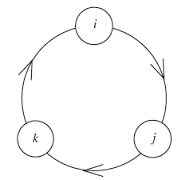
\includegraphics[scale=0.75]{images/kvaternioni.png}
  \caption{Diagram množenja kvaternionov}
\end{figure}

\begin{trditev}
  Z vpeljanim množenjem postane $\Ha$ realna algebra.
\end{trditev}

\begin{dokaz}
  Dokaz te trditve je rutinski.
\end{dokaz}

\begin{trditev}
  $\Ha$ je obseg.
\end{trditev}

\begin{dokaz}
  Vzemimo poljuben $0 \neq h \in \Ha$, kjer je $h = \alpha_0 + \alpha_1 i + \alpha_2 j + \alpha_3 k$.
  Vpeljimo konjugiran element $\overline{h} = \alpha_0 - \alpha_1 i - \alpha_2 j - \alpha_3 k$.
  Tedaj je $h \overline{h} = \overline{h} h = \alpha_0^2 + \alpha_1^2 + \alpha_2^2 + \alpha_3^2 > 0$.
  Sedaj pa lahko definiramo inverz kot $h^{-1} = \frac{1}{h \overline{h}} \overline{h}$.
\end{dokaz}

Elemente $\Ha$ imenujemo kvaternioni. $\Ha$ je nekomutativen obseg.
Izkaže se, da lahko v prostoru $\R \times \R^3$ vpeljemo definicijo množenja, ki je ekvivalentna množenju 
v $\Ha$:
$$(\alpha_0, \vec{u}) \cdot (\beta_0, \vec{v}) = (\alpha_0 \beta_0 - \vec{u} \cdot \vec{v}, \alpha_0 \vec{v} + \beta_0 \vec{u} + \vec{u} \times \vec{u}).$$
Definirajmo grupo za množenje $Q = \{\pm 1, \pm i, \pm j, \pm k\}$.
To je kvaternionska grupa, ki je z osmimi elementi druga najmanjša nekomutativna grupa za $S_3$
(izkazalo pa se bo, da ni edina nekomutativna grupa z 8 elementi).

Čeprav kvaternione ne obravnavamo kot števila, je množica $\Ha$ v nekem smislu naravni naslednik številskih množic 
$\N, \Z, \Q, \R, \C$. Na to namiguje dejstvo, da je $\Ha$ obseg.
Izkaže se, da so $\R$, $\C$ in $\Ha$ edine končnorazsežne realne algebre, ki so obsegi.
Njihove dimenzije so $1$, $2$ in $4$.
Če bi zaporedje nadaljevali, bi dobili množico oktonionov, 
ki ima veliko lepih lastnosti, vendar a v njej množenje ni več asociativno.

\subsection{Matrični kolobarji in linearne grupe}

Naj bo $n$ poljubno naravno število in $K$ poljuben (lahko celo nekomutativen) kolobar.
Potem lahko definiramo $M_n (K)$, t.j. množico $n \times n$ matrik 
z elementi iz $K$. Potem je $M_n (K)$ kolobar za običajni operaciji z matrikami.

Matrika $(a_{ij})$ se imenuje diagonalna matrika, če je $a_{ij} = 0$ za vse $i \neq j$.
Če je $a_{ij} \neq 0$ za vse $i > j$, potem matriki $(a_{ij})$ pravimo zgoraj trikotna matrika.
Če so hkrati tudi njeni diagonalci ničelni, je to strogo zgornje trikotna matrika.
Podobno vpeljemo (strogo) spodnje trikotne matrike.

Element $e$ kolobarja je idempotent, če je $e^2 = e$.
V tem primeru je tudi $1- e$ idempotent.
Očitna primera idempotentov v kolobarju sta $0$ in $1$, ki pa sta tudi edina v kolobarjih brez deliteljev niča.
Primer idempotenta v kolobarju $M_n (K)$ je na primer vsaka diagonalna matrika, ki ima na diagonali zgolj ničle in enice.

Element $a$ iz kolobarja je nilpotent, če je $a^n = 0$ za nek $n \in \N$.
Očitno je v kolobarjih brez deliteljev niča edini nilpotent kar ničla sama.
Primer nilpotentnega elementa v $M_n (K)$ je vsaka strogo zgoraj (ali spodaj)
trikotna matrika. Opazimo, da lahko v $M_n (\R)$ vsako Jordanovo formo zapišemo kot linearno kombinacijo 
nilpotenov in idempotentov.
Če je $K$ algebra nad poljem $F$, potem je tudi $M_n (K)$ algebra nad $F$ za množenje s skalarji, definirano kot 
$\lambda (a_{ij}) = (\lambda a_{ij})$. Take primere smo že spoznali:
$M_n (\R)$ je realna algebra, $M_n (\C)$ pa kompleksna.

Sedaj si oglejmo matrične grupe, katerih elementi so matrike nad poljem, operacija pa je množenje.
Množica vseh $n \times n$ matrik nad poljem $F$ ni grupa, temveč le monoid.
Spomnimo se, da je množica vseh obrnljivih elementov monoida $S$ tvori grupo $S^*$.
Torej je množica $\mathrm{GL}_n (F) = M_n(F)^*$ grupa, imenovana splošna linearna grupa.
Za $n > 1$ je ta grupa nekomutativna. 

Sedaj vpeljimo pojem determinante matrike za poljubno polje $F$.
Determinanto matrike $A = (a_{ij}) \in M_n (F)$ vpeljemo kot 
$$\det(A) = \sum_{\sigma \in S_n} \textrm{sgn$(\sigma)$} a_{1 \sigma(1)} \dots a_{n \sigma(n)},$$
kjer $S_n$ označuje množico vseh permutacij, \(\textrm{sgn$(\sigma)$}\) pa predznak permutacije $\sigma$.
Za tsplošno vpeljano determinanto veljajo naslednje lastnosti:
\begin{itemize}
  \item $\det(I) = 1$.
  \item $\det(AB) = \det(A) \det(B)$.
  \item Matrika $A \in M_n (F)$ je obrnljiva natanko tedaj, ko je $\det (A) \neq 0$.
\end{itemize}

\begin{opomba}
  Prvi dve lastnosti veljata že, če polje $F$ nadomestimo s komutativnim kolobarjem $K$.
  Previdni pa moramo biti pri tretji točki: tam velja ekvivalenca takrat, ko je $\det (A)$ obrnljiv element v $K$.
\end{opomba}

Sedaj lahko splošno linearno grupo karakteriziramo kot $\mathrm{GL}_n (F) = \{A \in M_n (F)\ |\ \det (A) \neq 0\}$.
Iz zgoraj navedenih lastnosti sledi, da je tudi množica $\mathrm{SL}_n (F) = \{A \in M_n (F)\ |\ \det (A) = 1\}$ grupa za množenje matrik.
Pravimo je posebna linearna grupa. Podobno sledi tudi za naslednje množice:
\begin{itemize}
  \item $O_n (F) = \{A \in M_n (F)\ |\ A A^\top = I\}$ -- ortogonalna grupa.
  \item ${SO}_n (F) = \{A \in O_n (F)\ |\ \det (A) = 1\}$ -- posebna ortogonalna grupa.
  \item $U_n  = \{A \in M_n (\C)\ |\ A A^* = I \}$ -- unitarna grupa.
  \item ${SU}_n = \{A \in U_n\ |\ \det (A) = 1\}$ -- posebna unitarna grupa.
\end{itemize}

\begin{zgled}
  Omenimo še en poseben primer podgrupe $\mathrm{GL}_n (F)$. Naj bo 
  $$J = \begin{bmatrix}
    0 & I_n\\
    -I_n & 0
  \end{bmatrix} \in M_{2n}.$$
  Potem je množica $\mathrm{Sp}_{2n} (F) = \{A \in M_{2n} (F)\ |\ A^\top J A = J\}$ simplektična grupa.
\end{zgled}

\subsection{Kolobarji funkcij}

Naj bo $X$ neprazna množica. Potem množica $\{f: X \to \R\}$ postane kolobar za operaciji
$(f + g)(x) = f(x) + g(x)$ in $(fg)(x) = f(x) \cdot g(x)$ (hkrati pa tudi algebra za $(\lambda f)(x) = \lambda \cdot f(x)$).
Podobno je tudi $C(X) = \{f: X \to \R\ |\ \mathrm{\text{$f$ zvezna}}\}$ kolobar in algebra (množica $X$ je na primer $\R$ ali nek poljuben interval).
Enako velja za $C^1(X), C^2(X), \dots, C^\infty (X)$.

\begin{zgled}
  Algebro realnih polinomov lahko opišemo kot podalgebro algebre vseh funkcij iz $\R$ v $\R$,
  generirano z identično funkcijo $\mathrm{id}_\R$. Seveda pa tukaj besede algebra ne moremo zamenjati s kolobarjem.
\end{zgled}

Sedaj vzemimo $X = \N$. Potem dobimo algebro realnih zaporedij $(a_1, a_2, \dots)$.
Definiciji seštevanja in množenja sta običajni definiciji teh operacij na zaporedjih:
\begin{gather*}
  (a_1, a_2, \dots) + (b_1, b_2, \dots) = (a_1 + b_1, a_2 + b_2, \dots)\\
  (a_1, a_2, \dots) \cdot (b_1, b_2, \dots) = (a_1 b_1, a_2 b_2, \dots).
\end{gather*}
Tudi množica konvergentnih zaporedij $c$ in množica omejenih zaporedij $l^\infty$ sta algebri.
Če pa je množica $X$ končna oziroma velja $|X| = n$, potem lahko funkcijo $f:X \to \R$ predstavimo kar 
z $n$-terico vrednosti, ki jih zavzame. Tedaj lahko $K = \{f: X \to \R\}$ identificiramo z $\R$.

\subsection{Kolobarji polinomov}

Naj bo $K$ poljuben kolobar. Polinom s koeficienti iz $K$ je formalna vsota 
$f(X) = a_0 + a_1 X + \dots + a_n X^n$, kjer so $a_i$ elementi nekega kolobarja $K$.
Imenujemo jih koeficienti $f(X)$, $a_0$ in $a_n$ pa posebej prosti člen in vodilni koeficient.
Formalna definicija polinoma je zaporedje oblike $$(a_0, a_1, \dots, a_n, 0, 0, \dots)$$
oziroma vsota $\sum_{k \geq 0} a_k X^k$, kjer je $a_k = 0$ za vsa števila $k$, večja od nekega števila $m \in \N$.
Množica vseh polinomov $K[X]$ s koeficienti iz kolobarja $K$ postane kolobar, če vpeljemo operaciji
\begin{gather*}
  \sum_{k \geq 0} a_k X^k + \sum_{k \geq 0} b_k X^k = \sum_{k \geq 0} (a_k + b_k) X^k\\
  \left(\sum_{k \geq 0} a_k X^k\right) \cdot \left(\sum_{k \geq 0} b_k X^k\right)  = \sum_{k \geq 0} c_k X^k,
\end{gather*}
kjer je $c_k = a_0 b_k + a_1 b_{k-1} + \dots + a_k b_0$.

\begin{opomba}
  Omenimo še kolobar formalnih potenčnih vrst $K[[X]]$, kjer koeficienti $a_k$ niso nujno ničelni od nekod dalje.
  Operaciji seštevanja in množenja sta definirani enako kot v $K[X]$.
\end{opomba}

Stopnja polinoma $0 \neq f(X) = a_0 + a_1 X + \dots + a_n X^n$ je enaka $0$, če $a_n \neq 0$.
Tedaj pišemo $\mathrm{st} (f(X)) = n$.

\begin{trditev}
  Če $K$ nima deliteljev niča, za vsaka neničelna polinoma $f(X), g(X) \in K(X)$ velja 
  $\mathrm{st}(f(X) g(X)) = \mathrm{st} (f(X)) + \mathrm{st} (g(X))$.
\end{trditev}

Naj bo sedaj kolobar $K$ komutativen. Vrednost polinoma $f(X) = a_0 + a_1 X + \dots + a_n X^n$
v elementu $x \in K$ definiramo kot $f(x) = a_0 + a_1 x + \dots + a_n x^n$.
Vsakemu polinomu $f(X) \in K[X]$ priredimo polinomsko funkcijo $x \mapsto f(x)$.
To je preslikava iz $K$ v $K$, ki jo določa polinom $f(X)$.
Vendar pa ne velja obratno, saj polinom ni enolično določen s svojo polinomsko funkcijo.

\begin{zgled}
  Polinoma $0$ in $X + X^2$ imata kot elementa $\Z_2[X]$ isto polinomsko funkcijo in sicer ničelno funkcijo 
  $x \mapsto 0$ za vsak $x \in \Z_2$. 
\end{zgled}

Omenimo še polinome več spremenljivk. Ti so vsota monomov, pomnoženih s koeficienti iz kolobarja $K$.
Stopnja takega polinoma je najvišja stopnja monoma, ki nastopa v njem.
Operaciji seštevanja in množenja definiramo tako kot prej.

Povsem formalna definicija polinomov več spremenljivk je naslednja: kolobar polinomov 
v dveh spremenljivkah nad kolobarjem $K$ definiramo kot $K[X, Y] = (K[Y])[Y]$, njegovi elementi pa so 
polinomi $\sum_{j \geq 0} \left(\sum_{i \geq 0} a_{ij} X^i\right)Y^j$, kjer je le končno mnogo elementov $a_{ij}$ različnih od $0$, spremenljivki $X$ in $Y$ pa komutirata.
Induktivno lahko uvedemo splošno definicijo polinoma $n$ spremenljivk:
$$K[X_1, \dots, X_n] = \left(K[X_1, \dots, X_{n - 1}]\right) [X_n].$$

\subsection{Simetrične grupe}

Grupo vseh permutacij množice $\{1, 2, \dots, n\}$ označujemo s $S_n$ in ji pravimo simetrična grupa.
Operacija v tej grupi je komponiranje, torej je $\sigma \pi$ produkt permutacij $\sigma$ in $\pi$.
Enota v $S_n$ je identična preslikava, ki jo bomo označevali kar z $1$.
Permutacijo $\sigma \in S_n$ označimo kot 
$$\sigma = \begin{pmatrix}
  1 & 2 & \dots & n\\
  i_1 & i_2 & \dots & i_n
\end{pmatrix}.$$
Vseh permutacij množice $n$ elementov je $n!$, zato velja $|S_n| = n!$.
Transpozicija je permutacija, ki med seboj zamenja elementa $i$ in $j$ iz $\N_n$,
vse druge elemente pa preslika vase. Transpozicija je očitno sama sebi inverz.
Hitro preverimo, da permutacije med seboj ne komutirajo za $n \geq 3$.

\begin{trditev}
  Vsaka permutacija $\sigma \in S_n$ se da zapisati kot produkt transpozicij.
\end{trditev}

Iz te trditve sledi, da množica vseh transpozicij generira grupo $S_n$,
vendar pa zapis permutacije kot produkt transpozicij ni enoličen.

\begin{trditev}
  Če permutacijo $\sigma \in S_n$ lahko zapišemo kot produkt sodega (iz. lihega)
  števila transpozicij, potem ima tudi vsak drug zapis $\sigma$ v obliki produkta transpozicij 
  sodo oziroma liho število faktorjev.
\end{trditev}

\begin{dokaz}[Skica dokaza]
  Naj bo $f(X_1, \dots, X_n)$ polinom v $n$ spremenljivkah nad nekim kolobarjem. Za neko permutacijo $\sigma \in S_n$
  vpeljemo polinom $(\sigma f) (X_1, \dots, X_n) = f(X_{\sigma(1)}, \dots, X_{\sigma(n)})$.
  Za neko drugo permutacijo $\pi \in S_n$ dobimo $(\pi(\sigma f)) (X_1, \dots, X_n) = (\sigma f)(X_{\pi(1)}, \dots, X_{\pi(n)})$.
  Hitro dobimo enakost $(\pi(\sigma f)) (X_1, \dots, X_n) = ((\pi \sigma) f)(X_{\pi(1)}, \dots, X_{\pi(n)})$.
  Najti moramo tak polinom $f(X_1, \dots, X_n) \in \Z[X_1, \dots, X_n]$, da za vsako transpozicijo $\tau$
  velja $(\tau f)(X_1, \dots, X_n) = -f(X_1, \dots, X_n)$ in od tod sledi 
  $((\tau_1 \dots \tau_k) f)(X_1, \dots, X_n) = (-1)^k f(X_1, \dots, X_n)$ za poljubne transpozicije $\sigma_1, \dots, \sigma_k$.
  Iskani polinom pa je $f(X_1, \dots, X_n) = \prod_{i < j} (X_i - X_j)$.
\end{dokaz}

Soda permutacija je produkt sodega števila transpozicij, liha pa lihega števila transpozicij.
Predznak permutacije $\mathrm{sgn} (\sigma)$ je $1$, če je $\sigma$ soda in $-1$, če je $\sigma$ liha.
Potem velja $\mathrm{sgn(\sigma \pi)} = \mathrm{sgn (\sigma)} \mathrm{sgn (\sigma)}$ in $\mathrm{sgn (\sigma^{-1})}= \mathrm{sgn(\tau)}^{-1}$
za vse $\sigma, \pi \in S_n$. Opazimo, da je množica sodih permutacij zaprta za množenje in inverze, zato je podgrupa $S_n$.
Imenujemo jo alternirajoča grupa $A_n$ in velja $|A_n| = \frac{n!}{2}$.

Pri predmetu algebra 1 smo omenili drugačne gradnike permutacij, to so cikli.
Cikel dolžine $k$ imenujemo $k-$cikel in ga označimo kot $\begin{pmatrix}
  i_1 & i_2 & \dots & i_k
\end{pmatrix}$. Ciklom, med katerimi nobena dva ne vsebujeta skupnega elementa, imenujemo disjunktni cikli.

\begin{trditev}
  Vsaka permutacija $\sigma \in S_n$ se da zapisati kot produkt disjunktnih ciklov.
\end{trditev}

Tak zapis je enoličen do vrstnega reda ciklov natančno (disjunktni cikli med seboj komutirajo).

\subsection{Diedrske grupe}

Denimo, da imamo kvadrat v ravnini. Njegova oglišča označimo z $1$, $2$, $3$ in $4$ kot na sliki.
Kvadrat v prostoru poljubno premikamo in vrtimo in ga nato postavimo na prvotno mesto.
Zato oglišča morda zamenjajo mesto in taki transformaciji pravimo simetrija.
Nanjo lahko gledamo na permutacijo oglišč.
Ker je tako produkt dveh simetrij kot tudi inverz simetrije spet simetrija, je množica 
simetrij podgrupa simetrične grupe $S_4$. Pravimo ji diedrska grupa reda $8$.

Označimo vrtenje za $90^\circ$ v levo kot $r$ in zrcaljenje preko vodoravne osi kot $z$.
Potem ima ta grupa elemente $$D_8 = \{1, r, r^2, r^3, z, rz, r^2z, r^3z\}.$$
Elementa $r$ in $z$ očitno generirata grupo $D_8$. Ker je $rz \neq zr$, grupa ni Abelova.
Veljajo pa še zveze $r^4 = 1$, $z^2 = 1$ in $(rz)^2 =1$.

Na enak način lahko obravnavamo simetrije pravilnega $n$-kotnika za $n \geq 3$.
Tako grupo označimo z $D_{2n}$ in je generirana z rotacijo $r$ (za kot $\frac{360^\circ}{n}$)
in zrcaljenjem $z$.
Pri tem ponovno velja $r^n = 1$, $z^2 = 1$ in $(rz)^2 = 1$, od koder sledi $zr^i = r^{-i} z$.
Ta grupa ima elemente $$D_{2n} = \{1, r, \dots, r^{n - 1}, z, rz, \dots, r^{n-1}z\}.$$
Lahko pa definiramo diedrsko grupo tudi za $n = 2$ in $n = 1$.
V prvem primeru definiramo $D_{4}$ kot grupo simetrij pravokotnika, ki ni kvadrat.
Sestavljajo jo elementi $1$, $r$, $z$ in $rz$, kjer je $zr = rz$, zato je ta grupa Abelova.
Diedrsko grupo $D_2$ pa sestavljata elementa $1$ in $r$, kjer je $r^2 = 1$.

\clearpage
\section{Homomorfizmi}

\subsection{Izomorfnost grup in ciklične grupe}

\begin{zgled}
  Končno grupo lahko predstavimo s Cayleyevo tabelo.
  Če zapišemo Caylejevi tabeli za $(\Z_4, +)$ in grupo $\{1, -1, i, -i\}$ za seštevanje,
  ugotovimo, da sta zgradbi obeh tabel enaki. S stališča teorije grup se ti dve grupi torej sploh ne razlikujeta.
\end{zgled}

\begin{definicija}
  Naj bosta $G$ in $G'$ grupi. Bijektivna preslikava $\varphi: G \to G'$ je izomorfizem grup,
  če velja $\varphi (xy) = \varphi(x) \varphi(y)$. Grupi $G$ in $G'$ sta si izomorfni, če obstaja 
  izomorfizem iz $G$ v $G'$. Takrat pišemo $G \cong G'$.
\end{definicija}

\begin{trditev}
  Če je $\varphi$ izomorfizem iz $G$ v $G'$, je $\varphi^{-1}$ izomorfizem iz $G'$ v $G$.
\end{trditev}

\begin{zgled}
  Oglejmo si nekaj osnovnih primerov izomorfizmov.
  \begin{itemize}
    \item Za vsako grupo $G$ velja $G \cong G$. Najenostavnejši primer takega izomorfizma je identična preslikava $\mathrm{id}_{G}$.
    \item Vsaka netrivialna podgrupa grupe $(\Z, +)$ ji je izomorfna: za $n \geq 1$ je $(n \Z, +)$ izomorfizem preslikava $\varphi:\ x \mapsto nx$.
    \item Ker velja $e^{xy} = e^x e^y$, sta grupi $(\R, +)$ in $(\R^+, \cdot)$ izomorfni.
  \end{itemize}
\end{zgled}

\begin{definicija}
  Grupa $G$ je ciklična, če je generirana z enim samim elementom: $G = \langle a \rangle = \{a^k\ |\ k \in \Z\}$.
\end{definicija}

\begin{zgled}
  Primeri cikličnih grup so $U_4 = \gen{i}$, $\Z_4 = \gen{1}$, $\Z_n$ in $\Z$.
\end{zgled}

\begin{izrek}
  Vsaka ciklična grupa je izomorfna bodisi $\Z$ bodisi $\Z_n$ za nek $n \geq 1$.
\end{izrek}

\begin{dokaz}
  Naj bo $G = \gen{a} = \{a^k\ |\ k \in \Z\}$. Če so vsi elementi $a^k$ različni, potem iz $a^k = a^l$ sledi $k = l$.
  To pomeni, da je preslikava $\varphi: \Z \to G$ s predpisom $\varphi(k) = a^k$ injektivna.
  Seveda je $\varphi$ tudi surjektivna in hitro se prepričamo, da je res izomorfizem.

  Obravnavajmo drugo možnost, ko obstajata taki celi števili $k < l$, da je $a^k = a^l$.
  Torej je $a^{l-k} = 1$ in definirajmo $n$ kot najmanjše naravno število, za katerega je $a^n = 1$.
  Trdimo, da je $|G| = n$ in $G = \{1, a, \dots, a^{n-1}\}$.
  Če je $0 \leq p < q < n$, sta elementa $a^p$ in $a^q$ res različna, saj bi sicer za naravno število $q-p < n$ veljalo $a^{q-p} = 1$.
  Torej je $|G| \geq n$. Vzemimo sedaj poljuben element $a^k \in G$. Po osnovnem izreku o deljenju obstajata taki celi števili $q, r$,
  da je $k = qn + r$ in $0 < r \leq n$. Zato je $a^k = a^r$, s čimer smo dokazali našo trditev.
  Sedaj je očitno, da sta grupi $G$ in $\Z_n$ izomorfni.
\end{dokaz}

Ker imata izomorfni grupi isti red, je vsaka končna ciklična grupa 
reda $n$ izomorfna grupi $(\Z_n, +)$, vsaka neskončna ciklična grupa pa grupi $(\Z, +)$.

\begin{definicija}
  Element $a \in G$ ima končen red, če je $a^n = 1$ za nek $n \in \N$.
  Če je $n$ najmanjše naravno število s to lastnostjo, ima $a$ red natanko $n$.
  To je ekvivalentno dejstvu $|\gen{a}| = n$.
  Če $a$ nima končen red, ima neskončen red.
\end{definicija}

\begin{zgled}
  V grupi $(\Z_4, +)$ ima element $0$ red $1$, element $2$ red $2$, elementa $1$ in $3$ pa red $4$.
  Diedrska grupa $D_4$ ima prav tako $4$ elemente, vendar imajo razen enote vsi red enak $2$.
  Ker izomorfizem ohranja red vsakega elementa, grupi $\Z_4$ in $D_4$ nista izomorfni (grupa $D_4$ pa je izomorfna $(\Z_2 \oplus \Z_2, +)$).
\end{zgled}

\subsection{Izomorfnost vektorskih prostorov}

Vektorska prostora $V$ in $V'$ sta si izomorfna, če obstaja bijektivna linearna preslikava
$\varphi: V \to V'$. Tedaj je $\varphi$ izomorfizem vektorskih prostorov.

\begin{trditev}
  Če sta $V$ in $V'$ končnorazsežna, sta si izomorfna natanko tedaj, ko velja $\dim_F V = \dim_F V'$.
\end{trditev}

\begin{posledica}
  Vsak netrivialen končnorazsežen vektorski prostor nad poljem $F$ je izomorfen prostoru $F^n$.
\end{posledica}

\subsection{Pojem homomorfizma}

\begin{definicija}
  Preslikava $\varphi: A \to A'$ je 
  \begin{itemize}
    \item homomorfizem grup, če sta $A$ in $A'$ grupi in velja $\varphi(xy) = \varphi(x) \varphi(y)$ za vse $x, y \in A$.
    \item homomorfizem vektorskih prostorov, če sta $A$ in $A'$ vektorska prostora nad $F$ in je $\varphi (x + y) = \varphi(x) + \varphi(y)$ 
    in $\varphi(\lambda x) = \lambda \varphi(x)$ za vse $x,y \in A$, $\lambda \in F$.
    \item homomorfizem kolobarjev, če sta $A$ in $A'$ kolobarja in je $\phi(1) = 1$, $\varphi (x + y) = \varphi(x) + \varphi(y)$ 
    in $\varphi(xy) = \varphi(x) \varphi(y)$ za vse $x,y \in A$.
    \item homomorfizem algeber, če sta $A$ in $A'$ algebri nad $F$ in je $\phi(1) = 1$, $\varphi (x + y) = \varphi(x) + \varphi(y)$, $\varphi(\lambda x) = \lambda \varphi(x)$ 
    in $\varphi(xy) = \varphi(x) \varphi(y)$ za vse $x,y \in A$, $\lambda \in F$.
  \end{itemize}
\end{definicija}

Bijektivnemu homomorfizmu pravimo izomorfizem, surjektivnemu epimorfizem, 
injektivnemu pa monomorfizem ali vložitev.
Homomorfizmu iz $A$ v $A$ pravimo endomorfizem, bijektivnemu endomorfizmu pa avtomorfizem.

\begin{opomba}
  Če sta $A$ in $A'$ aditivni grupi, potem je $\varphi: A \to A'$ homomorfizem in $\varphi(x + y) = \varphi(x) + \varphi(y)$.
  Rečemo tudi, da je $\phi$ aditivna preslikava.
\end{opomba}

\begin{opomba}
  Za homomorfizme kolobarjev in algeber smo zahtevali, da slikajo enoto $1$ kolobarja (algebre) $A$ 
  v enoto $1$ kolobarja (algebre) $A'$. Tako na primer preslikava $\varphi: \R \to M_2 (\R)$ s predpisom 
  $$\varphi(x) = \begin{bmatrix}
    x & 0\\
    0 & 0
  \end{bmatrix}$$ ni homomorfizem, čeprav ohranja tako vsoto kot produkt.
\end{opomba}

\begin{opomba}
  Izraz vložitev za injektiven homomorfizem $\varphi: A \to A'$ uporabimo takrat, 
  ko $A$ identificiramo z zalogo vrednosti $\varphi$ znotraj $A'$.
  Tako lahko kolobar $K$ vložimo v $K[X]$ s predpisom $a \mapsto a + 0\cdot X + 0 \cdot X^2 + \dots$
  Podobno lahko polje realnih števil vložimo v polje kompleksnih števil s predpisom $x \mapsto x + i0$.
\end{opomba}

\begin{trditev}
  Kompozitum homomorfizmov je homomorfizem.
\end{trditev}

\begin{trditev}
  Inverzna preslikava izomorfizma je izomorfizem.
\end{trditev}

Očitno sledi, da je $\cong$ ekvivalenčna relacija.

\begin{trditev}
  Množica vseh avtomorfizmov grupe (kolobarja, vektorskega prostora, algebre) $A$ je grupa za komponiranje.
\end{trditev}

\begin{trditev}
  Če je $\varphi: G \to G'$ homomorfizem grup, je $\varphi(1) = 1$ in $\varphi(x^{-1}) = \varphi(x)^{-1}$.
\end{trditev}

\begin{dokaz}
  Po definiciji izomorfizma velja $\varphi(1) = \varphi(1)^2$ in po pravilu krajšanja sledi $1 = \varphi(1)$.
  Druga točka sledi direktno iz te ugotovitve.
\end{dokaz}

\begin{opomba}
  To lahko posplošimo na formulo $\varphi(x^n) = \varphi(x)^n$ za vsa cela števila $n$ 
  (oziroma $\varphi(nx) = n \varphi(x)$ v primeru aditivnih grup).
\end{opomba}

\begin{trditev}
  Če je $\varphi: K \to K'$ homomorfizem kolobarjev in je $x$ obrnljiv, je tudi $\varphi(x^{-1}) = \varphi(x)^{-1}$.
\end{trditev}

\begin{dokaz}
  Po predpostavki je $\varphi(1) = 1$ in hitro pokažemo, da je 
  $\varphi(x) \varphi(x^{-1}) = \varphi(x^{-1}) \varphi(x) = 1$.
\end{dokaz}

\begin{definicija}
  Zalogi vrednosti homomorfizma $\varphi: A \to A'$ pravimo slika homomorfizma in jo označujemo kot 
  $\im \varphi = \{\varphi(x)\ |\ x \in A\}$.
\end{definicija}

\begin{trditev}
  Slika homomorfizma grup (oz. kolobarjev, vektorskih prostorov algeber) je podgrupa (oz. podkolobar, podprostor, podalgebra).
\end{trditev}

\begin{dokaz}
  Naj bo $\varphi: G \to G'$ homomorfizem grup. Potem je $\im \varphi$ zaprta za množenje zaradi $\varphi(xy) = \varphi(x) \varphi(y)$ 
  in zaprta za inverze zaradi $\varphi(x)^{-1} = \varphi(x^{-1})$.
\end{dokaz}

\begin{definicija}
  Jedro homomorfizma grup $\varphi: G \to G'$ je $\ker \varphi = \{x \in G\ |\ \varphi(x) = 1\}$.
  Če gre za aditivno grupo, pa se ta definicija glasi $\ker \varphi = \{x \in G\ |\ \varphi(x) = 0\}$.
  Jedro homomorfizma koloberjev, vektorskih prostorov in algeber definiramo na slednji način.
\end{definicija}

\begin{trditev}
  Homomorfizem $\varphi$ je injektiven natanko tedaj, ko je $\ker \varphi$ trivialen.
\end{trditev}

\begin{dokaz}
  Naj bosta $G, G'$ grupi. Ker je $\varphi(1) = 1$, je $1 \in \ker \varphi$.
  Če je $\varphi$ injektiven, je $\ker \varphi = \{1\}$.
  Dokažimo še obrat. Naj bo $\ker \varphi = \{1\}.$ Potem je 
  \begin{align*}
    \varphi(x) = \varphi (y) &\Rightarrow \varphi(x) \varphi(y)^{-1} = 1\\
    &\Rightarrow \varphi(xy^{-1}) = 1\\
    &\Rightarrow x = y \qedhere
  \end{align*}
\end{dokaz}

Izomorfizmi imajo trivialno jedro in največjo možno sliko.
Njihovo nasprotje so trivialni homomorfizmi grup, ki vse elemente prve grupe preslika v enoto druge grupe.
Na podoben način lahko trivialne homomorfizme definiramo za kolobarje, vektorske prostore in algebre.

\subsection{Primeri homomorfizmov}

Navedimo nekaj zgledov homomorfizmov grup.

\begin{zgled}
  Naj bo $G$ Abelova grupa in $n \in \Z$. Potem je $\varphi (x) = x^n$ endomorfizem, saj velja 
  $$\varphi(xy) = (xy)^n \stackrel{\mathrm{G\ Abelova}}{=} x^n y^n = \phi(x) \phi(y).$$
  Za $n = 1$ je to seveda avtomorfizem. V Abelovi grupi imamo predpis $\varphi(x) = n x$.
\end{zgled}

\begin{zgled}
  Preslikava $z \mapsto |z|$ je epimorfizem iz grupe $\C^*$ v $\R^+$. Operacija v obeh grupah je seveda množenje.
  Jedro tega epimorfizma je enotska krožnica $\mathbb{T} = \{z \in \C\ |\ |z| = 1\}$.
\end{zgled}

\begin{zgled}
  Preslikava $\varphi(x) = e^{ix}$ je homomorfizem iz $\R$ v $\mathbb{T}$.
\end{zgled}

\begin{zgled}
  Iz formule $\sgn (\pi \sigma) = \sgn (\pi)\, \sgn (\sigma)$ direktno sledi, da je preslikava 
  $\sigma \mapsto \sgn (\sigma)$ epimorfizem iz simetrične grupe $S_n$ v grupo $\{1, -1\}$ z množenjem.
  Jedro $\varphi$ je alternirajoča grupa $A_n$.
\end{zgled}

\begin{zgled}
  Preslikava $A \mapsto \det A$ je epimorfizem iz splošne linearne grupe $\mathrm{GL}_n (F)$ v grupo $(F^*, \cdot)$,
  saj je determinanta matrike multiplikativna. Jedro tege homomorfizma je $\mathrm{SL}_n$.
\end{zgled}

\begin{zgled}
  Naj bo $G$ poljubna grupa in $a \in G$.
  Potem je $\varphi_a: G \to G$ s predpisom $\varphi_a (x) = a x a^{-1}$ bijektivni endomorfizem oziroma avtomorfizem.
  Rečemo mu notranji avtomorfizem. Ker je $\varphi_a \varphi_b = \varphi_{ab}$ in $\varphi_{a^{-1}} = \varphi_a^{-1}$, je množica vseh notranjih avtomorfizmov $\mathrm{Inn}(G)$ 
  podgrupa grupe vseh avtomorfizmov $\mathrm{Aut}(G)$.
\end{zgled}

Sedaj si oglejmo še primere homomorfizmov kolobarjev in algeber.

\begin{zgled}
  Naj bo $K$ kolobar.
  Vsak $a \in K$, ki je obrnljiv, porodi notranji avtomorfizem $\varphi_a(x) = a x a^{-1}$.
  Enako velja tudi za algebre.
\end{zgled}

\begin{zgled}
  Za naravno število $n$ je preslikava $\varphi: \Z \to \Z_n$ s predpisom $\phi(a) = [a]$ epimorfizem kolobarjev. 
\end{zgled}

\begin{zgled}
  Preslikava $\varphi: K[X] \to K$, ki polinomu $f(X)$ priredi njegov konstantni člen, je epimorfizem.
  To preslikavo lahko opišemo tudi kot preslikavo, ki vsakemu polinomu $f(X)$ priredi element $f(0).$
  Element $0$ lahko tu zamenjamo s poljubnim elementom $x \in K$ in dobimo 
  epimorfizem $f(X) \mapsto f(x)$ iz kolobarja $K[X]$ v $K$.
\end{zgled}

\begin{zgled}
  Podoben primer kot v prejšnjem zgledu lahko ponovimo na kolobarju $C[0, 1]$.
  Za poljubno število $x \in [0, 1]$ je $f \mapsto f(x)$ epimorfizem iz kolobarja $C[0, 1]$ v $\R$.
  Izkaže se, da je tovrstna preslikava celo homomorfizem algeber.
\end{zgled}

\begin{zgled}
  Naj bo $V$ vektorski prostor nad $F$. Z $\mathrm{End}_F (V)$ označimo množico vseh endomorfizmov prostora $V$.
  Pri algebri 1 smo dokazali, da je tovrstna množica algebra nad $F$ in je izomorfna $M_2 (F)$.
\end{zgled}

\begin{zgled}
  Oglejmo si štiri primere podkolobarjev kolobarja realnih oz. kompleksnih matrik velikosti $2 \times 2$.
  \begin{gather*}
    K_1 = \left\lbrace \begin{bmatrix}
      x & 0\\
      0 & x
    \end{bmatrix}\ |\ x \in \R \right\rbrace \cong \R,\\
    K_2 = \left\lbrace \begin{bmatrix}
      x & 0\\
      0 & y
    \end{bmatrix}\ |\ x, y \in \R \right\rbrace \cong \R^2,\\
    K_3= \left\lbrace \begin{bmatrix}
      x & y\\
      -y & x
    \end{bmatrix}\ |\ x, y \in \R \right\rbrace \cong \C,\\
    K_4 = \left\lbrace \begin{bmatrix}
      z & w\\
      -\overline{w} & \overline{z}
    \end{bmatrix}\ |\ z, w \in \C \right\rbrace \cong \Ha.\\
  \end{gather*}
\end{zgled}

\subsection{Cayleyev izrek in druge vložitve}

\begin{izrek}[Cayley]
  Vsako grupo lahko vložimo v neko simetrično grupo.
\end{izrek}

\begin{dokaz}
  Za vsak element $a \in G$ definirajmo $l_a: G \to G$, kjer je $l_a(x) = ax$.
  Hitro lahko preverimo, da je ta funkcija bijektivna, torej $l_a \in \mathrm{Sim}(G)$.
  Sedaj definiramo preslikavo $\varphi: G \to \mathrm{Sim}(G)$ s predpisom $\varphi(a) = l_a$.
  Potem velja $\varphi(ab) = l_{ab} = l_a \cdot l_b = \varphi(a) \varphi(b)$.
  Preslikava $\varphi$ je injektivna, saj je $\ker \varphi = \{\mathrm{id_G}\}$. Torej je $\varphi$ injektiven homomorfizem oziroma vložitev.
\end{dokaz}

Izrek nam pove, da bi brez škode za splošnost grupo lahko definirali kot množico permutacij, ki je zaprta za množenje in inverze.
Kot je razvidno iz dokaza, pa nam izrek pove še več: grupo $G$ lahko vložimo v simetrično grupo $\mathrm{Sim} (G)$.

\begin{posledica}
  Vsako končno grupo $G$ lahko vložimo v simetrično grupo $S_n$ za neki $n \in \N$.
\end{posledica}

\begin{definicija}
  Grupa $G$ deluje na množici $X$, če obstaja preslikava iz $G \times X$ v $X$,
  ki vskemu paru $(a, x)$ priredi element $a \cdot x$, tako da velja:
  \begin{itemize}
    \item $(ab) \cdot x = a \cdot (b \cdot x)$ za vse $a, b \in G$ in vse $x \in X$.
    \item $1 \cdot x = x$ za vse $x \in X$. 
  \end{itemize}
  Tej preslikavi potem pravimo delovanje grupe $G$ na množici $X$.
\end{definicija}

Pojem delovanja grupe na množici je ekvivalenten pojmu homomorfizma iz grupe 
v simetrično grupo. Res, če je $\varphi$ homomorfizem iz grupe $G$ v simetrično grupo $\mathrm{Sim} (X)$,
potem je s predpisom $a \cdot x = \varphi (a) (x)$ definirano delovanje $G$ na $X$.
Obratno, če je dano delovanje grupe $G$ na množici $X$, potem lahko definiramo 
homomorfizem $\varphi: G \to \mathrm{Sim} (X)$ kot $\varphi (a) (x) = a \cdot x$.
Grupa $G$ deluje na sama sebi z običajnim množenjem; prav to je delovanje, ki smo ga uporabili 
v dokazu Cayleyevega izreka.


Naj bo sedaj $M$ aditivna grupa in označimo z $\mathrm{End}\ (M)$ množico
vseh njenih endomorfizmov, torej vseh aditivnih preslikav iz $M$ vase.
Potem za $f, g \in \mathrm{End}\ (M)$ definiramo $f + g$ kot vsoto funkcij po točkah,
$fg$ pa kot kompozitum $f \circ g$. Za tako definirani operaciji je $\mathrm{End}\ (M)$ kolobar.

\begin{izrek}
  Vsak kolobar $K$ lahko vložimo v kolobar endomorfizmov neke aditivne grupe.
\end{izrek}

\begin{dokaz}
  Dokaz je podoben Cayleyevemu izreku, le da ima tokrat vlogo aditivne grupe kar kolobar $K$.
  Kot prej za $a \in K$ definiramo $l_a : K \to K$ kot $l_a (x) = ax$.
  Hitro preverimo, da je preslikava $\varphi: K \to \mathrm{End}\ (K)$ s predpisom 
  $\varphi (a) = l_a$ homomorfizem kolobarjev s trivialnim jedrom.
\end{dokaz}

Kot smo prej vpeljali pojem delovanja grupe na množici, lahko sedaj definiramo pojem 
modula $M$ nad kolobarjem $K$.

\begin{definicija}
  Aditivna grupa $M$ skupaj z zunanjo binarno operacijo $(a, m) \mapsto am$
  iz $K \times M$ v $M$ je modul nad kolobarjem $K$, če velja:
  \begin{itemize}
    \item $(a + b)m = am + bm$ za vse $a, b \in K$ in vse $m \in M$.
    \item $a(m + n) = am + an$ za vse $a \in K$ in vse $m, n \in M$.
    \item $(ab)m = a (bm)$ za vse $a, b \in K$ in vse $m \in M$.
    \item $1m = m$ za vse $m \in M$. 
  \end{itemize}
\end{definicija}

Podobno kot prej je pojem modula ekvivalenten pojmu homomorfizma iz kolobarja $K$ v kolobar 
endomorfizmov aditivne grupe $M$.
Natančneje se modulu, ki smo ga vpeljali, reče levi modul. Desnega definiramo analogno.

\begin{izrek}
  Vsako algebro $A$ lahko vložimo v algebro endomorfizmov nekega vektorskega prostora.
\end{izrek}

Levi modul nad algebro $A$ definiramo kot vektorski prostor $M$, v katerem se poleg zahtev 
(i)-(iv) iz definicije modula nad kolobarjem dodamo še zahtevo, da je 
$\lambda (am) = (\lambda a) m =a (\lambda m)$ za vse $\lambda \in F$,
$a \in A$, $m \in M$.
Pojem modula nad algebro je ekvivalenten pojmu homomorfizma iz
algebre v algebro endomorfizmov vektorskega prostora.

V prejšnjem izreku za vektorski prostor seveda lahko izberemo kar $A$.
Če je $A$ končno-razsežna, lahko torej $A$ vložimo v algebro endomorfizmov 
končno-razsežnega vektorskega prostora, ta pa je izomorfna matrični 
algebri $M_n (F)$.

\begin{posledica}
  Vsako končno-razsežno algebro lahko vložimo v matrično 
  algebro $M_n (F)$ za neki $n \in \N$.
\end{posledica}

\begin{zgled}
  Ali lahko končno-razsežna algebra $A$ nad (denimo) $\R$ vsebuje 
  taka elementa $s$ in $t$, da je $st - ts = 1$?
  S prejšnjo posledico lahko ta problem pretvorimo v naslednje vprašanje: 
  ali obstajata takšni matriki $S, T \in M_n (\R)$, da je 
  $ST - TS = I$? Odgovor je ne, saj je sled matrike komutativna.
\end{zgled}

\subsection{Vložitev celega kolobarja}

Naj bo $K$ poljuben cel kolobar.

\begin{lema}
  S predpisom $(a, b) \sim (a', b') \Leftrightarrow ab' = a'b$
  je definirana ekvivalenčna relacija na množici $K \times (K \setminus \{0\})$.
\end{lema}

Vpeljimo oznako $\frac{a}{b}$ za ekvivalenčni razred elementa $(a, b)$.
Tu je $a$ poljuben element iz $K$ in $b$ poljuben element $K \setminus \{0\}$.
Takoj sledi, da je $\frac{a}{b} = \frac{a'}{b'} \Leftrightarrow ab' = a'b$.

\begin{lema}
  Za poljubne $a, a', c, c' \in K$ in $b, b', d, d' \in K \setminus \{0\}$
  iz $\frac{a}{b} = \frac{a'}{b'}$ in $\frac{c}{d} = \frac{c'}{d'}$ sledi 
  $\frac{ad + bc}{bd} = \frac{a'd' + b'c'}{b'd'}$ in $\frac{ac}{bd} = \frac{a'c'}{b'd'}$.
\end{lema}

\begin{izrek}
  Naj bo $K$ cel kolobar. Če v množico vseh ekvivalenčnih razredov
  $F = \left\lbrace \frac{a}{b} \Big|\ a, b \in K,\ b \neq 0 \right\rbrace$
  vpeljemo seštevanje in množenje s predpisoma $\frac{a}{b} + \frac{b}{d} = \frac{ad + bc}{bd}$
  in $\frac{a}{b} \cdot \frac{c}{d} = \frac{ac}{bd}$ postane $F$ polje.
  Preslikava $\varphi : K \to F$, definirana z $\varphi (a) = \frac{a}{1}$
\end{izrek}

\begin{dokaz}
  Po prejšnji lema sta operaciji seštevanja in množenja dobro definirani.
  To, da je $F$ polje, dokazujemo po definiciji. Da je $\varphi$ homomorfizem,
  sledi iz enakosti $\frac{a + b}{1} = \frac{a}{1} + \frac{b}{1}$ in $\frac{ab}{1} = \frac{a}{1} \cdot \frac{b}{1}$.
  Če je $\varphi(a) = 0$, je očitno $a = 0$, torej je $\varphi$ res tudi vložitev.
\end{dokaz}

\begin{definicija}
  Polje $F$ iz prejšnjega izreka se imenuje polje ulomkov nekega kolobarja $K$.
\end{definicija}

Kolobar $K$ obravnavamo kot podkolobar polja ulomkov $F$, pri čemer namesto $\frac{a}{1}$
pišemo kar $a$. Polje ulomkov celega kolobarja $K$ je generirano z množico $K$.


\begin{zgled}
  Navedimo nekaj zgledov.
  \begin{enumerate}
    \item Če je $K$ že samo polje, je $F = K$.
    \item Polje racionalnih števil $\Q$ je polje ulomkov kolobarja $\Z$.
    \item Kolobar polinomov več spremenljivk $F[X_1, \dots, X_n]$ je cel kolobar in njegovemu polju ulomkov 
    $F(X_1, \dots, X_n)$ pravimo polje racionalnih funkcij več spremenljivk.
  \end{enumerate}
\end{zgled}

\begin{posledica}
  Vsak cel kolobar lahko vložimo v polje.
\end{posledica}

Pri konstrukciji polja ulomkov smo večkrat uporabili komutativnost kolobarja $K$.
Izkaže se, da ne moremo vsakega nekomutativnega kolobarja brez deliteljev niča vložiti v (nekomutativen)
obseg.

\subsection{Karakteristika kolobarja in prapolja}

\begin{definicija}
  Naj bo $K$ kolobar. Če obstajajo taka naravna števila $n$, da je $n \cdot 1 = 0$,
  potem najmanjšemu izmed njih pravimo karakteristika kolobarja $K$.
  Če takih naravnih števil ni, pravimo, da ima kolobar $K$ karakteristiko $0$.
\end{definicija}

Kolobar je aditivna grupa za seštevanje in njegova karakteristika je enaka redu enote,
če je ta seveda končen, sicer pa je enaka $0$.
Ker je $n \cdot x = x + \dots + x = (1 + \dots + 1)x = (n \cdot 1)x$,
v kolobarju s karakteristiko $n$ velja $n \cdot x = 0$ za vse $x \in K$.

\begin{zgled}
  Večina kolobarjev, na katere najprej pomislimo, ima karakteristiko 
  $0$. Taki so na primer kolobarji $\Z$, $\Q$, $\R$ in $\C$.
  Kolobar ostankov $\Z_n$ pa ima karakteristiko $n$.
  Tudi kolobar polinomov $\Z_n [X]$, kolobar matrik $M_k (\Z_n)$
  in direktni produkt $\Z_n \times \Z_n$ imajo karakteristiko $n$.
\end{zgled}

\begin{zgled}
  Kolobar $\Z_3 \times \Z_2$ ima karakteristiko $6$.
\end{zgled}

\begin{trditev}
  Karakteristika neničelnega kolobarja $K$ brez deliteljev niča je bodisi $0$ bodisi praštevilo.
\end{trditev}

\begin{dokaz}
  Privzemimo, da je karakteristika $K$ naravno število $n$.
  Naj bo torej $n = rs$ za neki naravni števili $r$ in $s$.
  Potem je $(r \cdot 1)(s \cdot 1) = n \cdot 1 = 0.$
  Ker $K$ nima deliteljev niča, mora biti eden izmed elementov $r \cdot 1$
  in $s \cdot 1$ enak $0$. Po predpostavki je $n$ najmanjše naravno 
  število, za katerega je $n \cdot 1 = 0$. Zato sledi $r = n$ ali $s = n$.
  Torej je $n$ praštevilo.
\end{dokaz}

Polje ima torej lahko le praštevilsko ali ničelno karakteristiko.

\begin{izrek}
  Naj bo $F$ polje.
  \begin{enumerate}
    \item Če je karakteristika $F$ enaka $0$, lahko polje $\Q$ vložimo v $F$.
    \item Če je karakteristika $F$ praštevilo $p$, lahko polje $\Z_p$ vložimo v $F$.
  \end{enumerate}
\end{izrek}

\begin{dokaz}
  Naredimo doaz za prvo točko.
  Definiramo preslikavo $\varphi: \Q \to F$ s predpisom $\varphi \left(\frac{m}{n}\right) = (m \cdot 1)(n \cdot 1)^{-1}$
  za vse $m, n \in \Z$, $n \neq 0$. Dokazati moramo še dobro definiranost.
  Imamo:
  \begin{align*}
    \frac{m}{n} = \frac{m'}{n'} &\Rightarrow m n' = m' n\\
    &\Rightarrow (m \cdot 1) (n' \cdot 1) = (m' \cdot 1) (n \cdot 1)\\
    &\Rightarrow (m \cdot 1) (n \cdot 1)^{-1} = (m' \cdot 1) (n' \cdot 1)^{-1},
  \end{align*}
  kjer smo v zadnji vrstici uporabili predpostavko, da ima $F$ karakteritiko $0$.
  Tako smo pokazali, da je $\varphi$ dobro definirana preslikava.
  Z neposrednim računom pa preverimo tudi, da je homomorfizem s trivialnim jedrom.
  V drugi točki naredimo podoben dokaz, tako da definiramo 
  $\varphi : \Z_p \to F$ s predpisom $\varphi ([k]) = k \cdot 1$.
\end{dokaz}

Vsako podpolje vsebuje enoto $1$, zato je podpolje, generirano z $1$, najmanjše izmed vseh 
podpolj $F$. Imenujemo ga prapolje.
V dokazu izreka smo videli, da je v obeh primerih $\im \varphi$ enak prapolju polja $F$.
Torej lahko zaključimo, da če ima polje $F$ karakteristiko $0$, je njegovo prapolje izomorfno $\Q$,
če pa ima karakteristiko $p$, pa je njegovo prapolje izomorfno $\Z_p$.

\clearpage
\section{Kvocientne strukture}

\subsection{Odseki in Lagrangev izrek}

\begin{definicija}
  Naj bo $H$ podgrupa grupe $G$ in naj bo $a \in G$.
  Množici $a H = \{ah\ |\ h \in H$\} pravimo odsek grupe $G$ po podgrupi $H$.
\end{definicija}

Če je $G$ aditivna grupa, pišemo odsek kot $a + H$.
Odseki v splošnem niso podgrupe, saj če $a \neq H$, potem $a H$ ne vsebuje 
enote. Hkrati pa velja $aH = H \Leftrightarrow a \in H$, kar je enostavno dokazati.
Odsek $aH$ natančneje imenujemo levi odsek.
Desni odsek vpeljemo kot množico $Ha = \{ha\ |\ h \in H\}$.

\begin{zgled}
  Vpeljimo nekaj primerov odsekov.
  \begin{itemize}
    \item Naj bo $G = \Z$ in $H = n \Z$ za $n \in \N$.
    Odseki, ki jih porodijo $0, 1, \dots, n - 1$, so 
    $n\Z,\ 1 + n\Z,\ \dots\ ,(n - 1) + n\Z$.
    \item Naj bo $G$ aditivna grupa $\R^2$ in naj bo $H$ abscisna
    os, torej premica $y = 0$. Odseki $a + H$ so korizontalne premice, torej 
    premice vzporedne premici $H$.
    \item Naj bo $G = C^*$, tj. grupa neničelnih kompleksnih števil z operacijo množenja.
    Za $H$ vzemimo krožno grupo $\mathbb{T}$. Odsek $zH$ je množica 
    vseh kompleksnih števil. ki imajo isto absolutno vrednost kot število $z \in C^*$,
    torej so ti odseki koncentrične krožnice.
    \item Naj bo $G$ simetrična grupa $S_n$ in $H$ alternirajoča grupa $A_n$.
    Če je $\sigma \in H$, potem je $\sigma H = H$, sicer pa je $\sigma H$
    množica vseh lihih permutacij.
  \end{itemize}
\end{zgled}

\begin{lema}
  Za poljubna $a, b \in G$ velja $aH = bH \Leftrightarrow a^{-1} b \in H$.
\end{lema}

\begin{dokaz}
  Če je $aH = bH$, potem je $b = b \cdot 1 \in b H = a H$.
  Torej je $b = a h_0$ za neki $h_0 \in H$. To pa je ekvivalentno $a^{-1} b = h_0 \in H$.
  Obratno; naj bo $h_0 = a^{-1} b \in H$. Potem je $b = a h_0$ in zato 
  $bh = a(h_0 h) \in aH$ za vsak $h \in H$, torej $bH \subseteq aH$.
  Ker je $b^{-1} a = (a^{-1} b)^{-1} =h_0^{-1} \in H$, podobno vidimo, da je $a H \subseteq b H$.
\end{dokaz}

Če sta $a, b \in G$, potem je pogoj $a b^{-1} \in H$ ekvivalenten enakosti 
desnih odsekov $Ha$ in $Hb$. V aditivni grupi ugotovitev iz leme zapišemo kot
$a + H = b + H \Leftrightarrow b - a \in H \Leftrightarrow a - b \in H$.

\begin{lema}
  Za poljubna $a, b \in G$ sta odseka $aH$ in $bH$ bodisi enaka bodisi disjunktna. 
\end{lema}

\begin{dokaz}
  Denimo, da je $aH \cap bH \neq \emptyset.$
  Naj bosta $h_1, H_2 \in H$ taka, da je $a h_1 = b h_2$.
  Potem je $a^{-1} b = h_1 h_2^{-1} \in H$ in po lemi velja $aH = b H$.
\end{dokaz}

Grupa $G$ je torej disjunktna unija odsekov $aH$.
Tako lahko uvedemo ekvivalenčno relacijo s predpisom $a \sim b \Leftrightarrow a^{-1} b \in H$.

\begin{definicija}
  Moči množice vseh odsekov $\{aH\ |\ a \in G\}$ grupe $G$ po podgrupi 
  $H$ pravimo indeks podgrupe $H$ in jo označujemo z $[G : H]$.
\end{definicija}

Če je $G$ končna grupa, je seveda $[G : H] < \infty$ za vsako podgrupo $H$.
Tudi podgrupe neskončnih grup imajo lahko končen indeks, kot na primer 
$[\Z : n\Z] = n$.

\begin{izrek}[Lagrange]
  Naj bo $H$ podgrupa končne grupe $G$.
  Potem je $|G| = [G : H] \cdot |H|$.
\end{izrek}

\begin{dokaz}
  Naj bo $[G : H] = r$, potem lahko zapišemo množico vseh odsekov kot 
  $\{a_1 H, \dots, a_r H\}$ za neke $a_1, \dots, a_r \in G$.
  Hkrati pa vemo, da velja $|a_1 H| + \dots + |a_r H| = |G|$.
  Vsako izmed števil $|a_i H|$ pa je kar enako $|H|$, saj je
  preslikava $h \mapsto a_i h$ namreč bijekcija iz $H$ v $a_i H$.
  Torej je $|G| = r |H|$.
\end{dokaz}

Ta izrek nam pove, da je red končne grupe deljiv z redom vsake njene podgrupe.

\subsection{Podgrupe edinke in kvocientne grupe}

Naj bo $G$ poljubna grupa in $N$ njena podgrupa.
Označimo množico vseh odsekov kot $\quot{G}{N} = \{aN\ |\ a \in G\}.$
Intuitivno se zdi, da se s predpisom $aN \cdot bN = (ab) N$ ponuja operacija množenja
v tej množici. Vendar pa moraveljati določen pogoj, da je ta operacija dobro definirana.

\begin{lema}\label{lem:1}
  Naj bo $N$ podgrupa grupe $G$. Naslednja pogoja sta ekvivalentna.
  \begin{itemize}
    \item Za vse $a, a', b, b' \in G$ iz $aN = a'N$ in $bN = b'N$ sledi $(ab) N = (a'b') N$.
    \item Za vse $a \in G$ in $n \in N$ je $a n a^{-1} \in N$.
  \end{itemize}
\end{lema}

\begin{dokaz}
  Prvi pogoj lahko zapišemo kot 
  $$a^{-1}a' \in N\ \land\ b^{-1} b' \in N\ \Rightarrow b^{-1} a^{-1} a'b' \in N.$$
  Dokažimo $(i) \Rightarrow (ii)$. Za poljubna elementa $n \in N$ in $a \in G$
  je $1^{-1}n = n \in N$ in $a a^{-1} = 1 \in N$, zato je $a n a^{-1} = (a^{-1})^{-1} 1^{-1} n a^{-1} \in N$.
  Sedaj pa še $(ii) \Rightarrow (i)$. Naj bodo $a, a', b, b' \in G$ taki, 
  da je $n_1 = a^{-1}a' \in N$ in $n_2 = b^{-1} b' \in N$.
  Ker je $b^{-1} a^{-1} a' b' = (b^{-1} n_1 b) n_2$ in je $N$ podgrupa,
  sledi $b^{-1} a^{-1} a'b' \in N$.
\end{dokaz}

\begin{definicija}
  Če podgrupa $N$ grupe $G$ ustreza pogoju $(ii)$ iz leme \ref{lem:1},
  se imenuje podgrupa edinka in pišemo $N \lhd G$.
\end{definicija}

Hitro sledi, da je $N$ podgrupa edinka grupe $G$ natanko tedaj, ko je $N \leq G$ in $a N a^{-1} \subseteq N$
za vsak $a \in G$. Od tod pa takoj sledi naslednja trditev.

\begin{trditev}\label{trd:1}
  Za podgrupo $N$ grupe $G$ so naslednji pogoji ekvivalentni.
  \begin{enumerate}
    \item $N$ je edinka (tj. $a N a^{-1} \subseteq N$ za vsak $a \in G$)
    \item $aN \subseteq Na$ za vsak $a \in G$.
    \item $aN = N a$ za vsak $a \in G$.
    \item $a N a^{-1} = N$ za vsak $a \in G$.
  \end{enumerate}
\end{trditev}

Pogoj $(iv)$ je ekvivalenten temu, da je edina konjugirana 
podgrupa podgrupe $N$ podgrupa $N$ sama.

\begin{izrek}
  Naj bo $N \lhd G$. Če v množico $\quot{G}{N}$ vpeljemo množenje 
  s predpisom $aN \cdot bN = (a \cdot b) N$, postane $\quot{G}{N}$ grupa.
  Preslikava $\pi: G \to \quot{G}{N}$, definirana s $\pi (a) = aN$, 
  je epimorfizem in $\ker \pi = N$.
\end{izrek}

\begin{dokaz}
  Dobra definiranost množenja sledi iz leme \ref{lem:1},
  asociativnost pa je posledica asociativnosti množenja v $G$.
  Enota je odsek $N = 1 N$, inverz odseka $aN$ pa je $a^{-1} N$,
  zato je $\quot{G}{N}$ res grupa. Očitno je $\pi$ surjektiven homomorfizem.
  Vemo pa tudi, da velja $aN = N$ natanko tedaj, ko je $a \in N$,
  zato je $\ker \pi = N$.
\end{dokaz}

\begin{definicija}
  Grupi $\quot{G}{N}$ pravimo kvocientna ali faktorska grupa, preslikavi $\pi$
  pa kanonični epimorfizem.
\end{definicija}

Vsaka edinka je torej jedro nekega homomorfizma.
Pokazali bomo, da velja tudi obratno.

\begin{trditev}
  Podmnožica $N$ grupe $G$ je podgrupa edinka natanko tedaj, ko je $N$ jedro homomorfizma iz grupe $G$ v neko grupo $G'$.
\end{trditev}

\begin{dokaz}
  Dokažimo trditev v levo. Naj bo $N = \ker \varphi$ za neki homomorfizem 
  $\varphi: G \to G'$. Potem je $N$ tudi podgrupa.
  Za vsak $a \in G$ in vsak $n \in N$ je 
  $\varphi (a n a^{-1}) = \varphi(a) \varphi(n) \varphi(a)^{-1} = \varphi (a) 1 \varphi(a)^{-1} = 1$,
  torej $a N a^{-1} \subseteq N$ in $N$ je edinka.
\end{dokaz}

Vsaka netrivialna grupa $G$ ima vsaj dve podgrupi edinki, to sta $\{1\}$
in $G$. Če sta to tudi edini grupi edinki, je $G$ enostavna grupa.
Primer take grupe je na primer ciklična grupa praštevilskega reda in 
alternirajoča grupa $A_n$ za $n \geq 5$.

Če je $G$ končna grupa in $N \lhd G$, je po Lagrangevem izreku $|\quot{G}{N}| = \frac{|G|}{|N|}$.
Od tod med drugim sledi, da red kvocientne grupe deli red grupe.
V Abelovi grupi je očitno vsaka podgrupa edinka.
Primer je kvocientna grupa $\quot{\Z}{n\Z}$, ki je kar grupa ostankov $\Z_n$.

\begin{definicija}
  Če sta $H$ in $K$ podgrupi $G$, njun produkt definiramo kot množico 
  $HK = \{hk\ |\ h \in H,\ k \in K\}$.
\end{definicija}

V splošnem ta množica ni podgrupa.

\begin{trditev}\label{trd:3}
  Naj bo $G$ grupa.
  \begin{itemize}
    \item Če sta $H, K \leq G$ in je $HK = KH$, je $HK \leq G$.
    \item Če je $H \leq G$ in $N \lhd G$, je $HN = NH \leq G$.
    \item Če sta $M, N \lhd G$, je $MN = NM \lhd G$.
  \end{itemize}
\end{trditev}

\begin{dokaz}
  Dokažimo prvo točko.
  Vzemimo $h_1, h_2 \in H$ in $k_1, k_2 \in K$.
  Najprej moramo pokazati, da $(h_1 k_1)(h_2 k_2)^{-1} = h_1 k_1 k_2^{-1} h_2^{-1} \in HK$.
  Ker je $k_1 k_2 ^{-1} \in K$, $h_2^{-1} \in H$ in $KH = HK$, 
  je $k_1 k_2^{-1} h_2^{-1} = h_3 k_3$ za neka $h_3 \in H,\ k_3 \in K$.
  Torej je $h_1 k_1 k_2^{-1} h_2^{-1} = h_1 h_3 k_3 \in HK$.
  Druga točka sledi po trditvi \ref{trd:1}, saj je $hN = Nh$ za vsak $h \in H$ in zato je $HN = NH$.
  Tretjo točko pa dobimo, saj iz enakosti $a(mn)a^{-1} = (ama^{-1})(ana^{-1})$
  sledi $aMNa^{-1} \subseteq MN$ za vsak $a \in G$.
\end{dokaz}

Produkt podgrup Abelove grupe torej je podgrupa.
V aditivnih grupah namesto o produktu seveda govorimo o vsoti podgrup 
$H + K = \{h + k\ |\ h \in H,\ k \in K\}$.
Ne glede na to, ali je $G$ Abelova, pa je torej produkt edink spet edinka.
Kot lahko zlahka preverimo, enako velja za presek edink:
$$M \cap N \subseteq N, M \subseteq MN = NM$$
Naj bo sedaj komutator elementov $a$ in $b$ definiran kot $aba^{-1}b^{-1}$ in ga označimo z $[a, b]$.
Če $a$ in $b$ komutirata, je njun komutator enak $1$.

\begin{trditev}\label{trd:2}
  Če sta $M, N \lhd G$, je $[m, n] \in M \cap N$ za vse $m \in M$ in 
  $n \in N$. Iz $M \cap N = \{1\}$ tako sledi, da je $mn = nm$ za vse $m \in M$ 
  in $n \in N$.
\end{trditev}

\begin{dokaz}
  Če $[m, n]$ pišemo kot $m (n m^{-1} n^{-1})$ in upoštevamo, da je $M$ 
  podgrupa edinka, je $[m, n] \in M$. Podobno za $[m, n] \in N$.
\end{dokaz}

Nazadnje omenimo, da lahko govorimo tudi o produktu več podgrup.

\begin{definicija}
  Produkt podgrup $H_1, \dots, H_m$ grupe $G$ definiramo kot množico 
  $H_1H_2 \dots H_m = \{h_1 h_2 \dots h_m\ |\ h_i \in H_i,\ i = 1, \dots, m\}.$
\end{definicija}

Če so $N_1, \dots, N_m$ edinke, je edinka tudi $N_1 \dots N_m$.

\begin{lema}
  Naj bo $\varphi: G \to G'$ homomorfizem grup.
  \begin{itemize}
    \item Če je $H' \leq G'$, je $\varphi^{-1} (H') \leq G$.
    \item Če je $N' \lhd G'$, je $\varphi^{-1} (N') \lhd G$.
    \item Če je $H \leq G$, je $\varphi (H) \leq G'$.
    \item Če je $N \lhd G$ in je $\varphi$ epimorfizem, je $\varphi (N) \lhd G'$.
  \end{itemize}
\end{lema}

\begin{dokaz}
  Dokažimo prvo točko.
  Če sta $h, k \in \varphi^{-1} (H')$, potem sta $\varphi (h), \varphi(k) \in H'$.
  Od tod pa velja, da $\varphi (hk^{-1}) = \varphi (h) \varphi (k)^{-1} \in H'$ in zato je $hk^{-1} \in \varphi^{-1} (H')$.
  Dokažimo še drugo točko. Po prvi točke vemo, da je $\varphi^{-1} (N')$ podgrupa,
  moramo pokazati le, da iz $a \in G$ in $n \in \varphi^{-1} (N')$ sledi $a n a^{-1} \in \varphi^{-1} (N')$.
  To pa je res, saj je $\varphi(ana^{-1}) = \varphi(a) \varphi(n) \varphi(a)^{-1}$ in $N'$ je edinka.
  Preostali dve točki dokažemo podobno.
\end{dokaz}

Naj bo $N \lhd G$.
Če je $H$ podgrupa $G$, ki vsebuje $N$, potem je $N$ očitno tudi podgrupa edinka grupe $H$.
Zato lahko tvorimo kvocientno grupo $\quot{H}{N}$, ki pa je podgrupa $\quot{G}{N}$
(to sledi iz trditve (c), če vzamemo kanonični epimorfizem $\pi: G \to \quot{G}{N}$).
Podobno razmislimo, da je za vsako podgrupo edinko $M$ grupe $G$, ki vsebuje 
$N$, grupa $\quot{M}{N}$ podrgupa edinka grupe $\quot{G}{N}$.

\begin{izrek}\label{izr:1}
  Naj bo $N \lhd G$.
  \begin{itemize}
    \item Vsaka podgrupa $\quot{G}{N}$ je oblike $\quot{H}{N}$
    za neko podgrupo $H$ grupe $G$, ki vsebuje $N$.
    \item Vsaka podgrupa edinka grupe $\quot{G}{N}$ je oblike $\quot{M}{N}$
    za neko podgrupo edinko $M$ grupe $G$, ki vsebuje $N$.
  \end{itemize}
\end{izrek}

\begin{dokaz}
  Označimo z $\pi$ kanonični epimorfizem iz $G$ v $\quot{G}{N}$.
  Dokažimo najprej prvo točko. Naj bo $H'$ podgrupa $\quot{G}{N}$.
  Po prejšnji lemi je $H = \pi^{-1} (H')$ podgrupa grupe $G$.
  V $H$ so taki elementi $h$, za katere je $hN \in H'$. Zato je $N \subseteq H$,
  saj je $n N = N$ za vsak $n \in N$. Ker je preslikava $\pi$ surjektivna, 
  je $\pi (\pi^{-1} (H')) = H'$ in zato $H' = \pi (H) = \quot{H}{N}$.
  Dokaz drug točke poteka enako, le da vzamemo podgrupo edinko $N'$ grupe $\quot{G}{N}$
  in uporabimo drugo točko prejšnje leme. 
\end{dokaz}

\begin{zgled}
  Prejšnji izrek lahko uporabimo na podgrupah grupe $\Z_n = \quot{\Z}{n\Z}$.
  Ker je vsaka podgrupa grupe $\Z$ oblike $k\Z$ za nek $k \in \Z$, 
  je vsaka podgrupa grupe $\Z_n$ oblike $\quot{k\Z}{n\Z}$, kjer je $n\Z \subseteq k \Z$.
  To pa je izpolnjeno natanko tedaj, ko $k$ deli $n$, torej lahko grupo $\quot{k\Z}{n\Z}$
  zapišemo kot $k\Z$.
\end{zgled}

\subsection{Ideali in kvocientni kolobarji}

\begin{lema}
  Naj bo $I$ podgrupa za seštevanje $K$. Naslednja pogoja sta ekvivalentna.
  \begin{enumerate}
    \item Za vse $a, a', b, b' \in K$ iz $a + I = a' + I$ in $b + I = b' + I$ sledi $(ab) + I = (a' b') + I$.
    \item Za vse $a \in K$ in $u \in I$ je $au \in I$ in $ua \in I$.
  \end{enumerate}
\end{lema}

\begin{dokaz}
  Prvi pogoj lahko zapišemo tako, da iz $a' - a \in I$ in $b' - b \in I$ sledi $a'b' - ab \in I$.
  Začnimo s trditvijo v smeri $(i) \Rightarrow (ii)$. Za vsak $a \in K$ in $u \in I$
  velja $au = au - a0 \in I$ in $ua = ua - 0a \in I$.
  Sedaj pa še $(ii) \Rightarrow (i)$. Denimo, da za $a, a', b, b' \in K$ velja $u_1 = a' - a \in I$
  in $u_2 = b' - b \in I$. Iz $a'b' - ab = (a + u_1) (b + u_2) - ab = u_1 b + a u_2 + u_1 u_2$
  sledi $a'b' - ab \in I$.
\end{dokaz}

\begin{definicija}
  Naj bo $I$ podgrupa kolobarja $K$ za seštevanje.
  Če $I$ zadošča drugemu pogoju, se imenuje ideal kolobarja $K$.
  Tedaj pišemo $I \lhd K$.
\end{definicija}

Velja torej, da je $I \lhd K$ natanko tedaj, ko je $I$ podgrupa za seštevanje,
$KI \subseteq I$ in $IK \subseteq I$. Ideal je torej med drugim zaprt za množenje,
vendar pa praviloma ni podkolobar, saj ne vsebuje nujno enote $1$.
Če jo vsebuje, je pravzaprav enak celemu $K$.

\begin{zgled}
  Podmnožica kolobarja $\Z$ je ideal natanko tedaj, ko je $n \Z$ za $n \in \Z \cap \{0\}$.
\end{zgled}

\begin{izrek}
  Naj bo $I \lhd K$. Če v množico vseh odsekov $\quot{K}{I}$ vpeljemo seštevanje in množenje s 
  predpisoma $(a + I) + (b + I) = (a + b) + I$, $(a + I) (b + I) = ab + I$,
  postane $\quot{K}{I}$ kolobar. Preslikava $\pi: K \to \quot{K}{I}$,
  definirana s $\pi (a) = a + I$, je epimorfizem in $\ker \pi = I$.
\end{izrek}

\begin{dokaz}
  Iz prejšnjega razdelka vemo, da je $\quot{K}{I}$ aditivna grupa,
  množenje pa je dobro definirano po prejšnji lemi.
  Asociativnost in distributivnostna zakona sledita direktno iz 
  lastnosti $K$, enota za množenje pa je $1 + I$.
  Iz definicij seštevanja in množenja vidimo, da je 
  preslikava $\pi$ epimorfizem, hitro pa tudi sledi, da so v njegovem jedru natanko elementi iz $I$.
\end{dokaz}

\begin{definicija}
  Kolobarju $\quot{K}{I}$ pravimo kvocientni ali faktorski kolobar, preslikavi $\pi$
  pa kanonični epimorfizem.
\end{definicija}

\begin{zgled}
  Za primer vzemimo kolobar $\quot{\Z}{n\Z}$, ki pa je kot v primeru z grupami 
  enak $\Z_n$. Omenimo še očitna primera idealov poljubnega kolobarja $K$, 
  ki sta kar $\{0\}$ in $K$.
\end{zgled}

\begin{trditev}
  Podmnožica $I$ kolobarja $K$ je ideal natanko tedaj, ko je $I$ jedro homomorfizma iz kolobarja $K$ v neki kolobar $K'$.
\end{trditev}

\begin{dokaz}
  Vsak ideal je jedro kanoničnega epimorfizma. Dokazati moramo obratno trditev.
  Denimo, da je $I = \ker \varphi$ za neki homomorfizem $\varphi: K \to K'$.
  Če sta $u, v \in I$, je $\varphi(u - v) = \varphi(u) - \varphi (v) = 0$,
  torej $u - v \in I$ in $I$ je podgrupa.
  Za vsak $u \in I$ in $a \in K$ je $\varphi (au) = \varphi (a) \varphi (u) = \varphi (a) 0 = 0$
  in zato $au \in I$. Podobno vidimo, da je tudi $ua \in I$ in je zato $I$ ideal.
\end{dokaz}

Če sta $I$ in $J$ ideala kolobarja $K$, sta ideala tudi njun presek $I \cap J$ 
in vsota $I + J$. Prav tako je ideal njun produkt $IJ$, ki smo ga definirali kot podgrupo $K$ za seštevanje,
generirano z vsemi elementi oblike $uv$ za $u \in I$ in $v \in J$.
Če je kolobar $K$ nekomutativen, sta lahko ideala $IJ$ in $JI$ med seboj
različna. Oba pa sta po definiciji ideala vsebovana tako v $I$ kot v $J$.
Zato velja $IJ \subseteq I \cap J \subseteq I \subseteq I + J$.

\begin{definicija}
  Podmnožico $L$ kolobarja $K$ imenujemo levi ideal, če je podgrupa za seštevanje in če velja $KL \subseteq L$, 
  torej $al \in L$ za vse $a \in K$ in $l \in L$. Podobno definiramo 
  desni ideal, pri čemer zahtevamo $LK \subseteq L$.
\end{definicija}

Ideali so seveda hkrati levi in desni ideali, zato jim pravimo
dvostranski ideali. V komutativnih idealih vsi ti pojmi sovpadajo, v nekomutativnih pa v mnogih 
pomembnih ne.

\begin{zgled}
  Množica vseh matrik oblike $\begin{bmatrix}
    a & 0\\ b & 0
  \end{bmatrix}$ za $a, b \in \R$ je levi ideal kolobarja $M_2 (\R)$, 
  ki ni desni ideal. Obratno: množica matrik oblike 
  $\begin{bmatrix}
    a & b\\ 0 & 0
  \end{bmatrix}$.
\end{zgled}

\begin{trditev}
  Če levi ideal $L$ kolobarja $K$ vsebuje kak obrnljiv element, je $L = K$.
\end{trditev}

\begin{dokaz}
  Označimo obrnljiv element $l \in L$. Potem je $1 = l l^{-1} \in KL \subseteq L$
  in od tod $a = a1 \in KL \subseteq L$ za vsak $a \in K$.
\end{dokaz}

\begin{trditev}
  Neničeln kolobar $K$ je obseg natanko tedaj, ko sta $\{0\}$ in $K$ njegova edina leva ideala.
\end{trditev}

\begin{dokaz}
  Trditev v desno sledi direktno iz prejšnje trditve.
  Dokažimo trditev v nasprotno smer.
  Naj bosta $\{0\}$ in $K$ edina leva ideala kolobarja $K$.
  Vzemimo poljuben $a \neq 0$ iz $K$, potem je množica $Ka$ očitno levi ideal.
  Ker vsebuje $a = 1a$, ni enak $\{0\}$ in je zato po predpostavki enak $K$.
  Torej obstaja $b \in K$, da je $ba = 1$.
  Potem očitno $b \neq 0$ zato lahko vzamemo levi ideal $Kb$ in podobno zaključimo,
  da obstaja $c \in K$, da je $cb = 1$.
  Ker je levi inverz enak desnemu, je $ab = ba = 1$ in zato je poljuben neničeln element $K$ obrnljiv.
\end{dokaz}

\begin{definicija}
  Neničeln kolobar $K$ se imenuje enostaven kolobar, če sta $K$ in $\{0\}$
  njegova edina ideala.
\end{definicija}

Iz prejšnje trditve sledi, da so vsi obsegi enostavni kolobarji, vendar pa 
ta trditev ne velja v nasprotno smer; protiprimer je recimo kolobar $n \times n$ matrik nad obsegom.
V komutativnih kolobarjih pa ta dva pojma očitno sovpadata.

\begin{posledica}
  Komutativen kolobar $K$ je enostaven natanko tedaj, ko je polje.
\end{posledica}

\begin{lema}
  Naj bo $\varphi: K \to K'$ homomorfizem kolobarjev.
  \begin{itemize}
    \item Če je $I' \lhd K'$, je $\varphi^{-1} (I') \lhd K$.
    \item Če je $I \lhd K$ in je $\varphi$ epimorfizem, je $\varphi(I) \lhd K'$.
  \end{itemize}
\end{lema}

\begin{izrek}
  Naj bo $I \lhd K$. Vsak ideal kolobarja $\quot{K}{I}$ je oblike $\quot{J}{I}$
  za neki ideal $J$ kolobarja $K$, ki vsebuje $I$.
\end{izrek}

Seveda pa velja tudi obrat tega izreka, torej je $\quot{J}{I}$ ideal $\quot{K}{I}$
za vsak ideal $J$, ki vsebuje $I$.

\begin{definicija}
  Idealu $I$ kolobarja $K$ pravimo maksimalen ideal,
  če $I \neq K$ in če ne obstaja tak ideal $J$, da bi veljalo 
  $I \subseteq J \subseteq K$.
\end{definicija}

\begin{zgled}
  Trdimo, da je $2 \Z$ maksimalen ideal kolobarja $\Z$.
  Če namreč neki ideal kolobarja $\Z$ vsebuje vsa soda števila in še kakšno 
  liho število povrhu, potem je enak celemu kolobarju $\Z$.
\end{zgled}

\begin{posledica}
  Ideal $I$ kolobarja $K$ je maksimalen natanko tedaj, ko je kvocientni prostor $\quot{K}{I}$
  enostaven.
\end{posledica}

\begin{dokaz}
  Če je $I$ maksimalen, potem $\quot{K}{I}$ ni ničelni kolobar in 
  po prejšnjem izreku nima drugih idealov kot $\quot{I}{I} = \{0\}$
  in $\quot{K}{I}$, zato je $\quot{K}{I}$ enostaven.
  Obratno; če $I$ ni maksimalen, potem obstaja tak ideal $J$, da je 
  $I \subseteq J \subseteq K$ in tedaj je $\quot{J}{I}$
  tak ideal $\quot{K}{I}$, ki ni enak niti $\{0\}$ niti $\quot{K}{I}$,
  zato $\quot{K}{I}$ ni enostaven.
\end{dokaz}

\begin{posledica}
  Ideal $I$ komutativnega kolobarja $K$ je maksimalen natanko tedaj, 
  ko je kvocientni kolobar $\quot{K}{I}$ polje.
\end{posledica}

Omenimo še, da je vsak pravi ideal kolobarja vsebovan v nekem maksimalnem idealu.

\begin{definicija}
  Ideal algebre definiramo enako kot ideal kolobarja.
  Ker je za vsak skalar $\lambda$ in element $u$ iz ideala 
  algebre tudi $\lambda u = \lambda (1u) = (\lambda 1) u$ element ideala,
  je ideal podprostor.
\end{definicija}

\begin{izrek}
  Naj bo $U$ podprostor vektorskega prostora $V$.
  Če v množico vseh odsekov $\quot{V}{U}$ vpeljemo seštevanje in množenje s skalarji s predpisom 
  $(v + U) + (w + U) = (v + w) +U$ in $\lambda (v + U) = \lambda v + U$,
  postane $\quot{V}{U}$ vektorski prostor.
  Preslikava $\pi: V \to \quot{V}{U}$, definirana s $\pi (v) = v + U$
  je epimorfizem in $\ker \pi = U$.
\end{izrek}

Vektorskemu prostoru $\quot{V}{U}$ pravimo kvocientni ali faktorski vektorski prostor,
preslikavi $\pi$ pa kanonični epimorfizem.

\begin{izrek}
  Naj bo $I$ ideal algebre $A$.
  Če v množico $\quot{A}{I}$ vpeljemo 
  seštevanje, množenje in množenje s skalarji s predpisi 
  $(a + I) + (b + I) = (a + b) + I$, $(a + I)(b + I) = ab + I$
  in $\lambda (a + I) = \lambda a + I$, postane $\quot{A}{I}$ algebra.
  Preslikava $\pi: A \to \quot{A}{I}$, definirana s $\pi(a) = a + I$ je epimorfizem 
  in $\ker \pi = I$.
\end{izrek}

\subsection{Izrek o izomorfizmu in primeri kvocientnih prostorih}

\begin{izrek}
  Naj bo $\varphi: A \to A'$ homomorfizem (grup, kolobarjev, vektorskih prostorov ali algeber).
  Potem je $\quot{A}{\ker \varphi} \cong \im \varphi$.
\end{izrek}

\begin{dokaz}
  Obravnavajmo $\varphi$ kot homomorfizem grup.
  Kot vemo, je $\ker \varphi$ podgrupa edinka, zato lahko vpeljemo
  kvocientno grupo $\quot{A}{\ker \varphi}$. Za poljubna $a, a' \in A$ velja
  \begin{align*}
    a \ker \varphi = a' \ker \varphi &\Leftrightarrow a^{-1} a' \in \ker \varphi\\
    &\Leftrightarrow \varphi (a^{-1} a') = 0\\
    &\Leftrightarrow \varphi(a) = \varphi(a'). 
  \end{align*}
  Od tod sledi, da je preslikava $\overline{\varphi} : \quot{A}{\ker \varphi} \to \im \varphi$,
  definirana s predpisom $\overline{\varphi} (a \ker \varphi) = \varphi (a)$ dobro definirana
  in injektivna.
  Ker je 
  \begin{align*}
    \overline{\varphi} (a \ker \varphi \cdot b \ker \varphi) &= \overline{\varphi} ((ab) \ker \varphi)\\
    &= \varphi (ab) = \varphi(a) \varphi (b)\\
    &= \overline{\varphi} (a \ker \varphi) \overline{\varphi} (b \ker \varphi),
  \end{align*}
  je $\overline{\varphi}$ homomorfizem in je očitno tudi surjektiven.
\end{dokaz}

Pri dokazu smo implicitno uporabili naslednji komutativni diagram.
\begin{comment}
\[ \begin{tikzcd}
  A \arrow{r}{\pi} \arrow[swap]{dr}{\varphi} & \quot{A}{\ker \varphi} \arrow[d]{\overline{\varphi}} \\%
  & \im \varphi
  \end{tikzcd}
\]  }
\end{comment}
\begin{figure}[hbt!]
  \adjustbox{scale=1.2,center}{
      \begin{tikzcd}
        A \arrow[r, "\pi"] \arrow[dr, "\varphi"]
        & {\quot{A}{\ker \varphi}} \arrow[d, dashrightarrow, "\overline{\varphi}"]\\
        & \im \varphi
      \end{tikzcd}  
  }
    
\end{figure}

\begin{zgled}
  Oglejmo si preprost dokaz osnovnega izreka o cikličnih grupah.
  Naj bo $G$ ciklična grupa in $a \in G$ tak element, da je $G = \gen{a}$.
  Preslikava $\varphi: \Z \to G$ s predpisom $\varphi(n) = a^n$ je očitno epimorfizem grup.
  Če ima trivialno jedro, je izomorfizem, v nasprotnem primeru pa je $\ker \varphi = n \Z$
  za neki $n \in \N$. Po prejšnjem izreku je tedaj $\Z_n = \quot{\Z}{n\Z} \cong \im \varphi = G.$
\end{zgled}

\begin{zgled}
  Naj bo $G$ poljubna grupa. Potem sta podgrupi $\{1\}$ in $G$ edinki.
  Za ustrezni kvocientni grupi velja $\quot{G}{\{1\}} \cong G$ in $\quot{G}{G} \cong \{1\}$.
\end{zgled}

\begin{zgled}
  Naj bo $G$ aditivna grupa $\R^2$, $H$ pa premica $y = 0$, torej $H = \{(x_1, 0)\ |\ x_1 \in \R\}$.
  Potem je $H$ edinka in odseki so vodoravne premice.
  Vidimo, da je preslikava $(x_1, x_2) + H \mapsto x_2$ izomorfizem iz grupe $\quot{G}{H}$ v $\R$.
  Lahko pa do tega pridemo po drugi poti.
  Opazimo, da je preslikava $\varphi: G \to \R$ s predpisom $\varphi(x_1, x_2) = x_2$
  epimorfizem aditivnih grup in $\ker \varphi = H$. Zato po izreku velja $\quot{G}{H} \cong \R$.
\end{zgled}

\begin{zgled}
  Opišimo kvocientno grupo $\quot{\C^*}{\mathbb{T}}$. Za vsak $a \in \C^*$ lahko odsek $a \mathbb{T}$ 
  zapišemo kot $|a| \mathbb{T}$, produkt odsekov $a \mathbb{T}$ in $b \mathbb{T}$
  pa kot $|a||b| \mathbb{T}.$ Sklepamo, da je $\quot{\C^*}{\mathbb{T}} \cong \R^+$.
  Res, to sledi izizreka o izomorfizmu, saj je $z \mapsto |z|$ epimorfizem iz $\C^*$ 
  v $\R^+$ in njegovo jedro je $\mathbb{T}$.
\end{zgled}

\begin{zgled}
  Alternirajoča grupa $A_n$ je podgrupa edinka simetrične grupe $S_n$.
  To zelo hitro sledi iz dejstva, da je $A_n$ jedro epimorfizma $\sigma \mapsto \sgn \sigma$
  iz $S_n$ v grupo $(\{1, -1\}, \cdot)$. Od tod pa sledi, da je $\quot{S_n}{A_n} \cong \Z_2$
  in zato $[S_n : A_n] = 2$.
\end{zgled}

\begin{zgled}
  Posebna linearna grupa $\mathrm{SL}_n (F)$ je jedro epimorfizma $A \mapsto \det (A)$
  iz splošne linearne grupe $\mathrm{GL}_n (F)$ v grupo $(F^*, \cdot)$.
  Zato je $\quot{\mathrm{GL}_n (F)}{\mathrm{SL}_n (F)} \cong F^*$.
\end{zgled}

\begin{zgled}
  Center $Z(G)$ grupe $G$ je očitno podgrupa edinka.
  Torej lahko govorimo o kvocientni grupi $\quot{G}{Z(G)}$.
  V prejšnjem sklopu smo omenili, da je $a \mapsto \varphi_a$ epimorfizem iz grupe $G$ 
  v grupo notranjih avtomorfizmov $\mathrm{Inn} (G)$.
  V jedru te preslikave so elementi $c \in G$ z lastnostjo,
  da je $cxc^{-1} = x$ za vse $x \in G$, torej je jedro kar center $Z(G)$
  in je torej $\quot{G}{Z(G)} \cong \mathrm{Inn}(G)$.
\end{zgled}

\begin{opomba}
  Center $Z(G)$ grupe $G$ je edinka, center $Z(K)$ nekomutativnega kolobarja $K$ pa 
  ni ideal, saj vsebuje enoto.
\end{opomba}

Za naravno število $n \in \N$ so ekvivalentne naslednje izjave:
\begin{itemize}
  \item $p$ je praštevilo,
  \item kolobar $\Z_p = \quot{\Z}{p\Z}$ je polje in 
  \item $p\Z$ je maksimalen ideal kolobarja $\Z$.
\end{itemize}

\begin{zgled}
  Naj bo $K$ poljuben kolobar.
  Z $XK [X]$ označimo množico vseh polinomov iz $K[X]$ s konstantnim členom $0$.
  Potem je $XK [X]$ ideal $K[X]$ in $\quot{K[X]}{XK[X]} \cong K$.
  Če je $K$ polje, potem je ideal $XK[X]$ maksimalen.
\end{zgled}

\begin{zgled}
  Izberimo točko $x \in [0, 1]$.
  Množica $I_x = \{f \in C[0, 1]\ |\ f(x) = 0\}$ je ideal 
  kolobarja (oziroma algebre) $C[0, 1]$ in $\quot{C[0, 1]}{I_x} \cong \R$,
  torej je $I_x$ maksimalen ideal.
\end{zgled}

\begin{zgled}
  Naj bo $A$ končno generirana komutativna algebra nad poljem $F$.
  Če je $\{a_1, \dots, a_n\}$ množica njenih generatorjev, je torej 
  vsak element $A$ linearna kombinacija izrazov oblike $a_1 ^{k_1} \dots a_n^{k_n}$ za 
  $k_i \geq 0$. Torej je vsak element $A$ oblike $f(a_1, \dots, a_n)$,
  kjer je $f(X_1, \dots, X_n) \in F[X_1, \dots, X_n]$.
  Preslikava $\varphi: F[X_1, \dots, X_N] \to A$
  s predpisom $\varphi (f(X_1, \dots, X_n)) = f(a_1, \dots, a_n)$ je torej surjektivni homomorfizem algeber in 
  njegovo jedro $I$ je ideal.
  Po izreku o izomorfizmu je $\quot{F[X_1, \dots, X_n]}{I} \cong A$.
  Torej je vsaka komutativna algebra izomorfna kvocientni grupi algebre polinomov v $n$ spremenljivkah
  z nekim njenim idealom. Lahko bi vzeli tudi algebro polinomov neskončno mnogo spremenljivk 
  (le da so polinomi odvisni od končno mnogo spremenljivk).
  Torej lahko ta primer posplošimo, da je vsaka komutativna algebra izomorfna kvocientni grupi 
  algebre polinomov z nekim njenim idealom.
\end{zgled}

\subsection{Zunanji in notranji direktni produkti grup}

\begin{definicija}
  Grupa $G$ je notranji direktni produkt svojih podgrup
  edink $N_1, \dots, N_k$, če je $G = N_1 \dots N_m$ in če je 
  $$N_i \cap (N_1 \dots N_{i - 1} N_{i + 1} \dots N_m) = \{1\}$$
  za vse $i = 1, \dots, m$.
\end{definicija}

Če je grupa $G$ zunanji direktni produkt grup $G_1, \dots, G_m$, potem je $G$ notranji direktni produkt edink $\tilde{G}_i$,
kjer je $\tilde{G}_i = \{(1, \dots, 1, g_i, 1, \dots, 1)\ |\ g_i \in G_i\}$.
Dokazali bomo, da velja tudi obratno.

Iz definicije sledi, da je $N_i \cap N_j = \{1\}$ za vse $i \neq j$, zato je 
po trditvi \ref{trd:2} $n_i n_j = n_j n_i$ za vse $n_i \in N_i$, $n_j \in N_j$ ter $i \neq j$.
Prvi pogoj pove, da lahko vsak element iz $G$ zapišemo kot produkt elementov 
iz $N_1, \dots, N_m$ na vsaj en način, drugi pa nam zagotavlja, da je tak način le eden.

\begin{trditev}
  Grupa $G$ je notranji direktni produkt svojih podgrup edink $N_1, \dots, N_m$ 
  natanko tedaj, ko lahko vsak element iz $G$ na en sam način zapišemo kot $n_1 \dots n_m$,
  kjer je $n_i \in N_i$.
\end{trditev}

\begin{dokaz}
  Naj bo $G$ notranji direktni produkt podgrup edink $N_1, \dots, N_m$ in naj bo 
  $n_1 \dots n_m = r_1 \dots r_m$ za $n_i, r_i \in N_i$.
  To je ekvivalentno enakosti 
  $$r_1^{-1} n_1 = (r_2 \dots r_m) (n_2 \dots n_m)^{-1}.$$
  Ker je $N_2 \dots N_m$ po trditvi \ref{trd:3} podgrupa, vsebuje element $r_1^{-1} n_1$.
  Seveda je ta element vsebovan tudi v $N_1$, torej je $n_1 = r_1$.
  Po indukciji sledi, da velja $n_i = r_i$ za vsak $i = 1, \dots, m$.
  Dokažimo še obrat; naj se da vsak element iz $G$ samo na en način zapisati v obliki $n_1 \dots n_m$,
  kjer je $n_i \in N_i$.  
  Očitno velja prvi pogoj, zato se osredotočimo na drugega.
  Naj bo $a \in N_i \cap (N_1 \dots N_{i-1} N_{i + 1} \dots N_m)$.
  Potem lahko $a$ zapišemo na dva načina kot 
  $a = 1 \dots 1 \cdot n_i \cdot 1 \dots 1$ in 
  $a = n_1 \dots n_{i - 1} \cdot 1 \cdot n_{i + 1} \dots n_m$ za neke $n_j \in N_j$.
  Od tod pa takoj sledi, da je $a = 1$.
\end{dokaz} 

\begin{izrek}
  Če je grupa $G$ notranji direktni produkt svojih podgrup edink $N_1, \dots, N_m$,
  potem je $G$ izomorfna njihovemu zunanjemu direktnemu produktu $N_1 \times \dots \times N_m$.
\end{izrek}

\begin{dokaz}
  Vpeljimo preslikavo $\varphi: N_1 \times \dots \times N_m \to G$
  s predpisom $\varphi((n_1, \dots, n_m)) = n_1 \dots n_m$.
  Iz prejšnje trditve sledi, da je $\varphi$ bijektivna, hitro pa se da pokazati tudi, da je 
  homomorfizem.
\end{dokaz}

Notranji direktni produkt označujemo enako kot zunanjega in med njima v praksi sploh ne ločimo.
Naj bo $m = 2$.
Potem se pogoja iz definicije glasita $G = N_1 N_2$ in $N_1 \cap N_2 = \{1\}$.
Po prejšnji trditvi je to ekvivalentno temu, da lahko vsak element iz $G$ na en sam 
način zapišemo v obliki $n_1 n_2$, kjer je $n_1 \in N_1$ in $n_2 \in N_2$.
Torej je preslikava $\varphi: G \to N_2$ s predpisom $\varphi (n_1 n_2)$
dobro definirana, zlahko pa se prepričamo tudi, da je epimorfizem.
Ker je $\ker \varphi = N_1$, po izreku o izomorfizmu sledi $\quot{G}{N_1} \cong N_2$
(in analogno $\quot{G}{N_2} \cong N_1$).

\begin{zgled}
  Vsaka grupa $G$ je notranji direktni produkt svojih edink $G$ in $\{1\}$.
\end{zgled}

\begin{zgled}
  Diedrska grupa $D_4$ je notranji direktni produkt svojih (cikličnih) podgrup 
  $N_1 = \{1, r\}$ in $N_2 = \{1, z\}$ (ker je $D_4$ Abelova, so vse njene podgrupe edinke).
\end{zgled}

\begin{zgled}
  Grupa $\C^*$ je notranji direktni produkt svojih podgrup 
  $\R^+$ in $\mathbb{T}$. To je zato, ker lahko vsak $z \in \C^*$
  zapišemo kot $z = |z| \frac{z}{|z|}$, kjer je $|z| \in \R^+$ in $\frac{z}{|z|} \in \mathbb{T}$,
  hkrati pa je tudi $\R^+ \cap \mathbb{T} = \{1\}$.
  Potem sledi $\quot{\C^*}{\mathbb{T}} \cong \R^+$ oziroma $\quot{\C^*}{\R^+} = \mathbb{T}$,
  kar pa smo že pokazali.
\end{zgled}

\begin{zgled}
  Grupa $\mathrm{SL}_n (F)$ je podgrupa edinka grupe $\mathrm{GL}_n (F)$.
  Enako velja za grupo $Z$ vseh skalarnih matrik $\lambda I$, saj je le-ta center $\mathrm{GL}_n (F)$.
  Dokažimo, da če je $x \mapsto x^n$ bijektivna preslikava iz $F$ v $F$,
  potem je grupa $\mathrm{GL}_n (F)$ njun notranji direktni produkt.
  Res, naj bo $A \in \mathrm{GL}_n (F).$ Potem po predpostavki obstaja tak $\lambda \in F^*$,
  da je $\lambda^n = \det (A).$ 
  Tedaj je $\det (\lambda^{-1} A) = 1$ in posledično $\lambda^{-1} A \in \mathrm{SL}_n (F)$.
  Opazimo, da lahko $A$ zapišemo kot $A = \lambda I \cdot \lambda^{-1}$.
  Skalarna matrika $\lambda I$ leži v $\mathrm{SL}_n (F)$ natanko tedaj, ko je $\lambda^n = 1$.
  Ker je $x \mapsto x^n$ injektivna, je to natanko tedaj, ko je $\lambda = 1$.
  Torej je $Z \cap \mathrm{SL}_n (F) = \{I\}$.
\end{zgled}

V aditivnih grupah izraz direktni produkt zamenjamo z direktno vsoto.
Za aditivno grupo $G$ in njene podgrupe $N_i$ torej pišemo 
$G = N_1 \oplus \dots \oplus N_m$, kadar je $G = N_1 + \dots + N_m$
in $N_i \cap (N_1 + \dots + N_{i - 1} + N_{i + 1} + \dots N_m) = \{0\}$
za vse $i = 1, \dots, m.$

\begin{zgled}
  Grupa $\Z_6$ je notranja direktna vsota svojih podgrup $\{0, 2, 4\} \cong \Z_3$
  in $\{0, 3\} \cong \Z_2$, zato je $\Z_6 \cong \Z_3 \oplus \Z_2$.
  Grup $\Z_2$, $\Z_3$, $\Z_4$ in $\Z_5$ pa ne moremo razstaviti na direktne vsote praavih netrivialnih podgrup.
  Nekatere izmed naštetih grup jih pravzaprav sploh nimajo.
\end{zgled}

\subsection{Direktni produkti in vsote v kolobarjih}

\begin{definicija}
  Element kolobarja $K$ se imenuje idempotent, če je $e^2 = e$.
  Idempotent, ki komutira z vsakim elementom iz kolobarja (oziroma idempotent 
  iz centra kolobarja) se imenuje centralen idempotent.
\end{definicija}

Če je $e$ centralen idempotent, je $eK = \{ex\ |\ x \in K\}$ očitno ideal $K$.
Idempotenta $e$ in $f$ sta ortogonalna, če je $ef = fe = 0.$ Na primer, za vsak idempotent $e$
sta idempotenta $e$ in $1 - e$ ortogonalna.
Ortogonalni idempotenti imajo to lastnost, da je njihova vsota prav tako idempotent.

\begin{izrek}
  Naj bodo $I_1, \dots, I_m$ ideali kolobarja $K$.
  Potem je $K = I_1 \oplus \dots \oplus I_m$ natanko tedaj, ko obstajajo taki paroma ortogonalni 
  idempotenti $e_1, \dots, e_m \in K$, da je $e_1 + \dots + e_m = 1$ in $I_i = e_i K$ za vse $i = 1, \dots, m$.
\end{izrek}

\begin{dokaz}
  Dokažimo najprej implikacijo $(\Rightarrow)$.
  Naj bo $K = I_1 \oplus \dots \oplus I_m$.
  Potem je enota $1$ kolobarja enaka $e_i +\dots + e_m$, kjer je $e_i \in I_i$
  za vsak $i = 1, \dots, m$. Za vse $i \neq j$ je $I_i I_j \subseteq I_i \cap I_j = \{0\}$.
  Če pomnožimo enakost $1 = e_1 + \dots + e_m$ z leve (oziroma z desne) z 
  $u_i \in I_i$, dobimo $u_i = u_i e_i = e_i u_i$ za vse $u_i \in I_i$.
  Ta enakost nam pove, da je $I_i \subseteq e_i K$.
  Ker pa je $I_i$ ideal in $e_i \in I_i$, mora veljati tudi $e_i K \subseteq I_i$,
  torej je $I_i = e_i K$. 
  Če v prejšnjo enakost sedaj vstavimo $u_i = e_i$, vidimo, da je $e_i$ (centralen) idempotent.
  Ker je $I_i I_j = I_j I_i = \{0\}$ za $i \neq j$, velja $e_i u_j = u_j e_i = 0$
  za vse $u_j \in I_j$. Torej so $e_1, \dots, e_m$ paroma ortogonalni in smo dokazali.
  Dokaz v obratno smer $(\Leftarrow)$ je preprost.
\end{dokaz}

\begin{zgled}
  V prejšnjem zgledu smo omenili, da je grupa $(\Z_6, +)$ direktna vsota svojih 
  podgrup $\{0, 2, 4\}$ in $\{0, 3\}$. Ti podgrupi sta ideala kolobarja 
  $\Z_6$, ustrezna idempotenta pa sta $e_1 = 4$ in $e_2 = 1 - e_1 = 3$.
\end{zgled}

V prejšnjem dokazu v levo nismo potrebovali uporabiti dejstva, da so 
idempotenti $e_i$ centralni.
Torej smo pokazali, da je kolobar $K$ direktna vsota svojih desnih idealov 
$e_1 K, \dots, e_m K$, če so $e_i$ paroma ortogonalni idempotenti in je njihova vsota enaka $1$.
Ideali $I_i$ iz izreka niso podkolobarji $K$, saj ne vsebujejo enote $1$ kolobarja $K$.
So pa vendarle kolobarji s svojo enoto $e_i$, v nasprotju s splošnimi ideali kolobarjev,
ki pa nimajo nujno svojih enot. Zato lahko govorimo o 
direktnem produktu kolobarjev $I_1 \times \dots \times I_m$.

\begin{izrek}
  Če je kolobar $K$ enak direktni vsoti svojih idelov $I_1, \dots, I_m$, potem je $K$ izomorfen njihovemu produktu
  $I_1 \times \dots \times I_m$.
\end{izrek}

\begin{dokaz}
  Dokažimo, da je preslikava $\varphi: I_1 \times \dots \times I_m \to K$ s predpisom 
  $\varphi((u_1, \dots, u_m)) = u_1 + \dots + u_m$ homomorfizem kolobarjev.
  Ker lahko vsak element iz $K$ na natanko en način zapišemo kot $u_1 + \dots + u_m$ za $u_i \in I_i$,
  je $\varphi$ bijektivna. Dokažimo še, da je multiplikativna.
  Hočemo, da je za poljubne $u_i, v_i \in I_i$ element 
  $$\varphi((u_1, \dots, u_m) \cdot (v_1, \dots, v_m)) = \varphi (u_1 v_1, \dots, u_m v_m) = u_1 v_1 + \dots + u_m v_m$$
  enak elementu 
  $$\varphi(u_1, \dots, u_m) \cdot \varphi (v_1, \dots, v_m) = (u_1 + \dots + u_m) (v_1 + \dots + v_m).$$
  To pa je takojšnja posledica dejstva, da je $u_i v_j = (u_i e_i) (e_j v_j) = 0$ za $i \neq j$.
\end{dokaz}
Vse, kar smo povedali za produkte in vsote v kolobarjih, velja tudi za algebre.

\clearpage
\section{Končne grupe}

\subsection{Posledice Lagrangevega izreka}

\begin{izrek}[Lagrange]
  Če je $G$ končna grupa in $H$ njena podgrupa, potem je $|G| = [G:H] \cdot |H|$.
\end{izrek}

Pri tem je $[G: H]$ indeks grupe $G$ po podgrupi $H$, torej število vseh odsekov $aH$
za $a \in G$. Največkrat uporabljamo naslednjo posledico izreka.

\begin{posledica}
  Red vsake končne podgrupe deli red grupe.
\end{posledica}

\begin{posledica}\label{pos:1}
  Naj bo $a$ element grupe $G$.
  \begin{itemize}
    \item Če ima $a$ red $n$, potem za vsak $m \in \Z$ velja $a^m = 1 \Leftrightarrow n\ |\ m$.
    \item Če je $a \neq 1$ in za neko praštevilo $p$ velja $a^p = 1$, potem je $p$ red elementa $a$.
    \item Če ima $a$ red $n$ in je $\varphi: G \to G'$ homomorfizem grup, potem red elementa $\varphi(a)$ deli $n$.
    \item Če je $N$ edinka v $G$ in ima $a$ red $n$, potem red $aN \in \quot{G}{N}$ deli $n$.
  \end{itemize}
\end{posledica}

\begin{posledica}
  Red vsakega elementa končne grupe deli red grupe.
\end{posledica}

\begin{dokaz}
  Red elementa $a$ je enak redu ciklične podgrupe $\gen{a}$, ki pa po Lagrangevem izreku deli red grupe.
\end{dokaz}

\begin{posledica}
  Če je $G$ končna grupa z $n$ elementi, je $a^n = 1$ za vsak $a \in G$.
\end{posledica}

\begin{posledica}
  Za vsako praštevilo $p$ in naravno število $a$ je $a^p \equiv a \Mod{p}$.
\end{posledica}

\begin{dokaz}
  Privzemimo, da $p$ ne deli $a$. Elementi polja $\Z_p$ so odseki $x + p\Z$,
  kjer je $x \in \Z$. Potem je element $a + p\Z$ neničeln in zato element 
  grupe $\Z_p^*$. Po prejšnji posledici je $(a + p\Z)^{p -1} = 1 + p\Z$,
  kar pa je ekvivalentno $a^{p-1} + p\Z = 1 + p\Z$ oziroma $a^{p-1} -1 \in p\Z$.
  Trditev je dokazana.
\end{dokaz}

\begin{posledica}
  Vsaka grupa $G$ s praštevilskim redom je ciklična.
  Še več, za vsak element $a \in G \setminus \{1\}$ je $\gen{a} = G$.
\end{posledica}

Vsaka grupa $G$ s $p$ elementi je torej izomorfna grupi $(\Z_p, +)$.

\begin{posledica}
  Netrivialna grupa nima pravih netrivialnih podgrup natanko tedaj, ko je ciklična grupa s praštevilskim redom.
\end{posledica}

\begin{dokaz}
  $(\Rightarrow)$ Naj bo $G$ netrivialna grupa brez pravih netrivialnih podgrup.
  Potem je $\gen{a} = G$ za vsak $a \in G \setminus \{1\}$.
  Torej je $G$ ciklična grupa in zato izomorfna bodisi $\Z$ bodisi $\Z_n$ za nek $n \in \N$.
  Ker ima $\Z$ prave netrivialne podgrupe, pride v poštev le druga možnost: $G \cong \Z_n$.
  Če $n$ ni praštevilo oziroma je deljiva s številom $d$, kjer je $1 < d < n$, 
  potem je $d\Z_n$ njena prava netrivialna množica in smo prišli v protislovje.
  Obrat $(\Leftarrow)$ je očiten.
\end{dokaz}


\subsection{Razredna formula}

\begin{definicija}
  Elementa $a$ in $a'$ iz grupe $G$ sta si konjugirana,
  če obstaja tak $g \in G$, da je $a' = g ag^{-1}$.
\end{definicija}

Očitno je konjugiranost ekvivalenčna relacija na $G$.
Ta relacija na $G$ porodi razpad množice $G$ na ekvivalenčne razrede.
Imenujemo jih konjugiranostni razredi.
Če je grupa $G$ končna, velja $|G| = \sum_i |R_i|$,
kjer so $R_i$ konjugiranostni razredi.
To formulo bomo preoblikovali, da bo dobila želeno obliko.
Za poljuben element $a \in G$ naj $R(a)$ označuje konjugiranostni razred, ki mu $a$ pripada,
torej $R(a) = \{gag^{-1}\ |\ g \in G\}$.
Vpeljimo še množico $C(a) = \{g \in G\ |\ ag = ga\}$ vseh elementov $G$, ki komutirajo z $a$.
Imenujemo jo centralizator elementa $a$.
Poleg elementa $a$ očitno vsebuje tudi vse elemente iz centra $Z(G)$ grupe $G$.

\begin{lema}
  Za vsak element $a$ iz grupe $G$ je njegov centralizator $C(a)$ podgrupa $G$
  in velja $|R(a)| = [G: C(a)]$.
\end{lema}

\begin{dokaz}
  Očitno je, da je $C(a)$ podgrupa.
  Za poljubna $g, h \in G$ velja $gC(a) = hC(a)$ natanko tedaj, ko je 
  $g^{-1} h \in C(a)$, torej ko je $g^{-1} h a = a g^{-1} h$.
  To pa lahko preoblikujemo v $g ag^{-1} = h a h^{-1}$.
  Torej velja $gag^{-1} = h a h^{-1} \Leftrightarrow g C(a) = h C(a)$.
  To pa pomeni, da je $g a g^{-1} \mapsto gC(a)$ dobro definirana injektivna preslikava 
  iz $R(a)$ v množico vseh odsekov $G$ po podgrupi $C(a)$.
  Ker je ta preslikava očitno surjektivna, smo na koncu dokaza.
\end{dokaz}

Omenimo še, da če je $a \in Z(G)$, je očitno $R(a) = \{a\}$ in $C(a) = G$.
Velja tudi $a \in Z(G) \Leftrightarrow  |R(a)| = 1$.
Sedaj lahko prejšnjo enakost zapišemo kot $|G| = |Z(G)| + \sum_j |R_j|$,
kjer so $R_j$ konjugiranostni razredi z več kot enim elementom, torej razredi,
katerih elementi ne ležijo v centru. Sedaj uporabimo še prejšnjo lemo.

\begin{izrek}
  Naj bo $G$ končna grupa. Potem obstajajo taki $a_j \in \quot{G}{Z(G)}$,
  da velja $|G| = |Z(G)| + \sum_j [G : C(a_j)]$.
\end{izrek}

Tej enakosti pravimo razredna formula.

\subsection{Cauchyjev izrek}

Naj bo $G$ končna grupa.
Po Lagrangevem izreku je red vsakega elementa iz $G$ število, ki deli red $G$.
Ali velja tudi obratno? V splošnem ne, saj če $G$ ni ciklična grupa, potem ne vsebuje 
elementa reda $|G|$. Vendar pa se izkaže, da je odgovor pritrdilen,
če je $n$ praštevilo.

\begin{izrek}[Cauchy]
  Naj bo $G$ končna grupa. Če praštevilo $p$ deli $|G|$, potem $G$ vsebuje element
  reda $p$.
\end{izrek}

\begin{dokaz}
  Izrek dokažimo z indukcijo na $n = |G|$.
  Če je $p = n$, potem je $G$ ciklična grupa in ima 
  vsak njen element red $p$.
  Privzemimo torej, da je $n > p$ in da izrek velja za vse grupe 
  z manj kot $n$ elementi, torej tudi za vse prave podgrupe grupe $G$.

  Najprej obravnavajmo primer, ko $G$ ni Abelova.
  Potem je njen center $Z(G)$ prava podgrupa in če je $p\ |\ |Z(G)|$,
  potem smo že končali. Predpostavimo torej, da $p$ ne deli $|Z(G)|$.
  Iz razredne formule sledi, da $p$ ne deli $[G: C(a_j)]$ za neki $a_j \in \quot{G}{Z(G)}$.
  Po Lagrangu je $n = [G: C(a_j)] \cdot |C(a_j)|$, zato mora $p$ deliti $|C(a_j)|$.
  Ker pa je $C(a_j)$ prava podgrupa $G$, dokaz sledi iz indukcijske predpostavke.
  
  Oglejmo si še primer, ko $G$ je Abelova.
  Ker $|G|$ ni praštevilo, mora $G$ po eni izmed posledic vsebovati
  kako pravo netrivialno podgrupo $N$.
  Zaradi komutativnosti $G$ velja $N \lhd G$ in zato po Lagrangu $|G| = |\quot{G}{N}| \cdot |N|$.
  Če je $p\ |\ N$, potem smo po indukcijski predpostavki že končali.
  Naj bo torej $p\ |\ |\quot{G}{N}|$. Ker ima $\quot{G}{N}$ manj kot $n$ elementov,
  po indukcijski predpostavki vsebuje element $aN$, ki ima red $p$.
  Po posledici \ref{pos:1} (d) je $a \in G$ element reda $m = kp$
  in je zato $a^k$ element reda $p$.
\end{dokaz}

\begin{definicija}
  Naj bo $p$ praštevilo.
  Grupa $G$ se imenuje $p$-grupa, če je red vsakega njenega elementa potenca števila $p$.
\end{definicija}

\begin{posledica}
  Končna grupa $G$ je $p$-grupa natanko tedaj, ko je 
  $|G| = p^m$ za neki $m \in \N$.
\end{posledica}

\begin{zgled}
  Primeri $p$-grup so ciklične grupe $\Z_p$, $\Z_{p^2}$ in tako naprej.
  Prav tako sta kvaternionska grupa $Q$ in diedrska grupa $D_8$ $2$-grupi.
  Direktni produkt $p$-grup je spet $p$-grupa, enako velja tudi za podgrupe $p$-grup.
\end{zgled}

\subsection{Delovanja grup}

\begin{definicija}
  Grupa $G$ deluje na množici $X$, če obstaja taka preslikava iz $G \times X$ v $X$,
  ki vsakemu paru $(a, x)$ priredi element $a \cdot x$, da velja:
  \begin{itemize}
    \item $a \cdot (b \cdot x) = (ab) x$ za vse $a, b \in G$ in $x \in X$.
    \item $1 \cdot x = x$ za vsak $x \in X$.
  \end{itemize}
  Tej preslikavi rečemo delovanje $G$ na $X$.
\end{definicija}

\begin{zgled}
  Navedimo nekaj zgledov delovanja.
  \begin{enumerate}
    \item $G$ deluje na $G$ z običajnim množenjem.
    \item $G$ deluje na $G$ s konjugiranjem: $a \cdot x = a x a^{-1}$.
    \item Naj bo $H \leq G$ in $X$ množica vseh odsekov $xH$ za $x \in G$.
    Potem $G$ deluje na $X$ kot $a \cdot xH = (ax)H$.
    \item $G$ deluje na množici vseh njenih podgrup kot $a \cdot K = a K a^{-1}$.
    \item Grupa $S_n$ deluje na $\{1, \dots, n\}$ kot $\sigma \cdot i = \sigma(i)$.
    \item Grupa $\mathrm{GL}_n (\R)$ deluje na $\R^n$ kot $A \cdot v = Av$.
    \item Trivalno delovanje: $a \cdot x = x.$
  \end{enumerate}
\end{zgled}

\begin{definicija}
  Naj $G$ deluje na $X$.
  Orbita elementa $x \in X$ je množica
  $G \cdot x = \{ a \cdot x\ |\ a \in G\}$, stabilizator elementa 
  $x \in X$ pa množica $G_x = \{a \in G\ |\ a \cdot x = x\}$.
\end{definicija}

\begin{zgled}
  Naj $G$ deluje nase s konjugiranjem.
  Potem je orbita $G \cdot x = R(x)$ in stabilizator $G_x = C(x)$.
\end{zgled}

Hitro se da pokazati, da je stabilizator vselej podgrupa: $G_x \leq G$.
S predpisom $x \sim y \Leftrightarrow x = a \cdot y$ za nek $a \in G$
je definirana ekvivalenčna relacija na $X$. Ekvivalenčni razred, v katerem leži $x$,
je orbita $G \cdot x$.
V podpoglavju o razredni formuli smo izpeljali rezultat (lemo), ki nam je dala enakost 
$|R(x)| = [G: C(x)]$. Sedaj lahko izpeljemo njeno posplošitev.

\begin{lema}
  Naj $G$ deluje na $X$.
  Potem je $|G \cdot x| = [G : G_x]$ za vse $x \in X$.
\end{lema}

\begin{dokaz}
  Za vse $a, b \in G$ je 
  \begin{align*}
    a \cdot x = b \cdot x &\Leftrightarrow b^{-1} a \cdot x = x\\
    &\Leftrightarrow b^{-1} a \in G_x\\
    &\Leftrightarrow a G_x = b G_x.
  \end{align*}
  Sedaj ponovno definiramo preslikavo $a \cdot x \mapsto a \cdot G_x$
  iz množice $G \cdot x$ v množico vseh odsekov po $G_x$ in po prejšnjem razmisleku 
  je ta preslikava injektivna in dobro definirana. Seveda pa je tudi surjektivna.
  To je lema o orbiti in stabilizatorju.
\end{dokaz}

\begin{izrek}
  Naj grupa $G$ deluje na končni množici $X$. Označimo z $Z$
  množico vseh $x \in X$, za katere velja $a \cdot x = x$ za vse $a \in G$.
  Potem obstajajo taki $x_1, \dots, x_m \in X \setminus Z$, da je $|X| = |Z| + \sum_{j = 1} ^m [G : G_{x_j}]$.
  Če je $G$ končna $p$-grupa, je $|X| \equiv |Z| \Mod{p}.$
\end{izrek}

\begin{dokaz}
  Dokaz poteka skoraj enako kot v razdelku o razredni formuli.
  Opazimo, da je $x \in Z \Leftrightarrow |G \cdot x| = 1$.
  Orbite so ekvivalenčni razredi, zato je $|X|= |Z| + \sum_{j = 1} ^m |G \cdot x_j|$, kjer smo
  uporabili prejšnjo lemo. Če je $G$ končna $p$-grupa, potem je 
  $|G \cdot x| = [G : G_{x_j}] = \frac{|G|}{|G_{x_j}|} = p^l$ za $l \in \N$,
  zato je $p\ |\ |X| - |R|$.
\end{dokaz}

\subsection{Izreki Sylowa}

Po Lagrangevem izreku vemo, da če je $H$ podgrupa $G$, potem velja $|H|\ |\ |G|$.
Kljub temu, da v splošnem obrat te trditve ne velja, pa iz 
Cauchyjevega izreka vemo, da če je $p$ praštevilo in $p$ deli $|G|$,
potem $G$ vsebuje grupo reda $p$. Ali lahko gremo še dlje?

\begin{zgled}
  Vzemimo alternirajočo grupo $A_4$ z redom $|A_4| = 12$.
  Pokažemo lahko, da $A_4$ ne vsebuje grupe, ki bi imela red $6$. 
\end{zgled}

Naj bo $H \leq G$. Množici $N_G (H) = \{a \in G\ |\ aHa^{-1} = H\}$
pravimo normalizator $H$. Očitno velja $H \lhd G \Leftrightarrow N_G (H) = G$,
izkaže pa se tudi, da je normalizator $H$ podgrupa v $G$ in velja 
$H \lhd N_G (H) \leq G$.

\begin{definicija}
  Naj bo $G$ končna grupa. Njena podgrupa $H \leq G$ je $p$-podgrupa, če je $|H| = p^l$
  za neki $l \geq 0$. 
  Naprej; $H$ je $p$-podgrupa Sylowa, če je $|H| = p^k$ in $p^{k + 1}$ ne deli $|G|$.
\end{definicija}

\begin{izrek}[Izreki Sylowa]
  Naj bo $G$ končna grupa in $p$ praštevilo, ki deli $|G|.$
  \begin{enumerate}
    \item Če $p^l$ deli $|G|$, potem $G$ vsebuje vsaj eno $p$-podgrupo reda $p^l$.
    \item Vsaka $p$-podgrupa je vsebovana v kakšni $p$-podgrupi Sylowa.
    \item Poljubni $p$-podgrupi Sylowa sta si konjugirani.
    \item Število vseh $p$-podgrup Sylowa deli red $|G|$.
    \item Število vseh $p$-podgrup Sylowa je oblike $mp + 1$ za $m \geq 0$.
  \end{enumerate}
\end{izrek}

\begin{dokaz}
  Dokaz točke (1): ponovno naredimo dokaz po indukciji na $|G| = n$,
  torej naj trditev velja za vse grupe z manj kot $n$ elementi.
  Najprej obravnavamo primer, ko $p$ ne deli $|Z(G)|$.
  Potem po razredni formuli obstaja tak $x_j \in G$,
  da $p$ ne deli $[G: C(x_j)]$.
  Po Lagrangu je $n = |G| = |G: C(x_j)| |C(x_j)|$ in ker je $p^l\ |\ n$, sledi $p^l\ |\ |C(x_j)|.$
  Ker je $C(x_j)$ prava podgrupa, moramo le še uporabiti indukcijsko predpostavko in smo končali.
  Obravnavajmo še primer $p\ |\ |Z(G)|$. Potem po Cauchyjevem izreku obstaja tak $c \in Z(G)$,
  da je $c \neq 1$ in $c^p = 1.$ Potem je $\gen{c} \lhd G$ in velja 
  $|\quot{G}{\gen{c}}| = \frac{|G|}{p} < m$ ter $p^{l-1}\ |\ |\quot{G}{\gen{c}}|$, zato lahko uporabimo indukcijsko 
  predpostavko ima $\quot{G}{\gen{c}}$ podgrupo reda $p^{l-1}$ oblike $\quot{H}{\gen{c}}$
  za $\gen{c} \leq H \leq G$.
  Potem je $|H| = |\quot{H}{\gen{c}}| \cdot |\gen{c}| = p^{l-1} \cdot p = p^l$ in $H$ je iskana podgrupa.

  Dokaz točk (2) in (3):
  naj bo $S$ $p$-podgrupa Sylowa in $X = \{xS\ |\ x \in G\}$.
  Definirajmo delovanje neke $p$-podgrupe $H$ na $X$ kot $a \cdot xS = (ax)S$
  za $a \in H$ in $x \in G$. Definirajmo $Z$ kot množico vseh takih odsekov $xS$,
  da je $a \cdot xS = xS$ za vsak $a \in H$.
  Ker je $H$ $p$-grupa, velja $|X| \equiv |Z| \Mod{p}$.
  Ker je po Lagrangu $|X| = \quot{|G|}{|S|}$ in $p$ ne deli $X$,
  potem $p$ tudi ne deli $Z$. Torej $Z$ ni prazna in obstaja $xS \in Z$.
  Torej za vsak $a \in H$ velja $axS = xS$, od tod pa sledi $x^{-1} a x \in S$ za vsak $a \in H$.
  Takoj dobimo $H \subseteq x S x^{-1}$ in očitno je $|xSx^{-1}| = |S|$.
  Torej je $xSx^{-1}$ taka $p$-podgrupa, ki vsebuje $H$.
  Od tod takoj sledi tudi točka (3), torej če vzamemo, da je $H$ $p$-podgrupa Sylowa.

  Dokaz točke (4): naj bo $Y$ množica vseh $p$-podgrup Sylowa, torej
  $Y = \{xSx^{-1}\ |\ x \in G\}$. Definirajmo delovanje $G$ na $Y$ s konjugiranjem:
  $a \cdot T = a T a^{-1}$ za vsak $a \in G$.
  Potem je orbita $S$ kar cela množica $Y$, njen stabilizator pa je normalizator
  $N_G (S) = \{a \in G\ |\ aSa^{-1} = S\}$.
  Po lemi o stabilizatorju in orbiti je $|G| = |Y| |N_G (S)|$, torej 
  $|Y|\ |\ |G|$ in smo dokazali.

  Dokaz točke (5): naj $S$ deluje na $Y$ kot prej, torej 
  $a \cdot T = a T a^{-1}$ za $a \in S$.
  Naj bo $W$ množica vseh elementov $T \in Y$,
  da je $a \cdot T = T$ za vsak $a \in S$.
  To je ekvivalentno temu, da je $S \subseteq N_G (T)$ in zato je $S \in W$.
  Vzemimo sedaj nek $T \in W$. $S$ in $T$ sta
  $p$-podgrupi Sylowa grupe $N_G (T)$. Torej sta si $S$ in $T$ konjugirani 
  in zato je $S = a T a^{-1}$ za neki $a \in N_G (T)$.
  Ker pa je $a T a^{-1} = T$, je $S = T$ in zato je $W = \{S\}$.
  Sedaj pa dobimo $|Y| \equiv |W| = 1 \Mod{p}$.
\end{dokaz}

\begin{zgled}
  Denimo, da je $|G| = pq$, kjer sta $p$ in $q$ praštevili in $p < q$.
  Predpostavimo še, da $p$ ne deli $q - 1$.
  Potem obstaja natanko ena $p$-podgrupa Sylowa in natanko ena $q$-podgrupa Sylowa.
  Poimenujmo ti grupi $M$ in $N$. Očitno sta $M$ in $N$ podgrupi edinki.
  Ker je $|M| = p$, $|N| = q$ in $|M \cap N|$ deli $|M|$ in $|N|$,
  mora biti $|M \cap N| = \{1\}$.
  Hkrati lahko uporabimo dejstvo, da imata $M$ in $N$ praštevilsko moč in 
  sta zato ciklični grupi; $M = \gen{a}$ in $N = \gen{b}$.
  Ker je presek edink $M$ in $N$ trivialen, vsak element iz $M$ komutira z vsakim elementom iz $N$.
  Potem sledi $(ab)^{pq} = 1$ in takoj lahko pokažemo, da je red tega elementa kar $pq = |G|$.
  Torej je grupa $G$ ciklična.
\end{zgled}

  Zanima nas problem klasifikacije končnih grup.
  Edina grupa (do izomorfizma natančno) z dvema elementoma je na primer $\Z_2$,
  edina s tremi elementi pa $\Z_3$. Hitro lahko pokažemo, da je poljubna grupa 
  $G = \{1, a, b, c\}$ s štirimi elementi izomorfna bodisi $\Z_4$ bodisi $\Z_2 \oplus \Z_2$.
  Res, če ima vsaj eden od $a, b, c$ red 4, potem je $G \cong \Z_4$,
  sicer pa imajo $a, b, c$ vse red 2 in hitro sledi, da je v tem primeru $G \cong \Z_2 \oplus \Z_2.$
  Vsaka grupa s 5 elementi je izomorfna $\Z_5$, saj je 5 preštevilo.
  Omenimo še, da je vsaka grupa s 6 elementi izomorfna $\Z_3 \oplus \Z_2$
  ali $S_3$, vsaka grupa s 7 elementi je izomorfna $\Z_7$,
  vsaka grupa z 8 elementi pa $\Z_8$, $\Z_4 \oplus \Z_2$, $\Z_2 \oplus \Z_2 \oplus \Z_2$,
  $D_8$ ali $Q$.

  Z naraščanjem števila elementov ta problem postaja čedalje bolj zahteven.
  Omejimo se na končne enostavne grupe. Vemo že, da so te lahko oblike 
  $\Z_p$, kjer je $p$ praštevilo, ali pa na primer alternirajoče grupe $A_n$ za $n \geq 5$.
  Grupa $A_5$ je pravzaprav najmanjša nekomutativna enostavna grupa.
  Izkaže se, da lahko končne enostavne grupe klasificiramo v 18 neskončnih družin 
  in 26 izjem, ki jim pravimo sporadične grupe. Največja izmed teh se imenuje monster group
  in ima približno $8 \cdot 10^{55}$ elementov. To pa so tudi vse.
  Te grupe imajo mnoge zanimive lastnosti - ena izmed njih je recimo ta,
  da imajo vse sodi red.

\subsection{Končne Abelove grupe}

Poznamo že ciklične grupe $\Z_n$ in njihove direktne vsote.
Izkaže se, da so take oblike prav vse končne Abelove grupe.
V tem razdelku obravnavamo aditivne grupe $(G, +)$, 
v katerih velja $m \cdot a = 0$ natanko tedaj, ko red elementa $a$ deli $m$.

\begin{lema}
  Naj bo $|G| = mn$, kjer sta si $m$ in $n$ tuji števili.
  Naj bo $H = \{x \in G\ |\ mx = 0\}$ in $K = \{x \in G\ |\ nx = 0\}$.
  Potem sta $H$ in $K$ podgrupi in $G = H \oplus K$. 
\end{lema}

\begin{dokaz}
  Očitno sta $H$ in $K$ res podgrupi.
  Če sta $m$ in $n$ tuji, potem obstajata $u, v \in \Z$,
  da je $um + vn = 1$. Torej je 
  $$x = 1 \cdot x = u(mx) + v(nx)$$ in je $G = H + K$.
  Dokazati moramo še $H \cap K = \{0\}$.
  Če je $x \in H \cap K$, potem je $mx = nx = 0$ in iz zgornje enačbe takoj sledi $x = 0$.
\end{dokaz}

\begin{opomba}
  Iz te leme takoj sledi, da imamo razcep $\Z_6 = \Z_3 \oplus \Z_2$,
  saj sta si števili $3$ in $2$ tuji.
\end{opomba}

\begin{lema}
  Denimo, da je $|G| = p_1^{k_1} \dots p_r^{k_r}$, kjer so $p_i$ paroma različna praštevila.
  Potem je $G = H_1 \oplus H_2 \oplus \dots \oplus H_r$, kjer je $|H_i| = p_i^{k_i}$
  za vsak $i = 1, \dots, r$.
\end{lema}

Z zgornjima lemama lahko podamo razcep končnih Abelovih grup, ki imajo na primer 
red $42 = 2 \cdot 3 \cdot 7$. Res, če je $|G| = 42$, potem je $G = \Z_2 \oplus \Z_3 \oplus \Z_7$.
Kaj pa na primer $|G| = 16$? Odslej se osredotočimo na $p$-grupe.

\begin{lema}
  Naj bo $G$ $p$-grupa. Potem je $G$ ciklična natanko tedaj, ko vsebuje samo eno 
  podgrupo reda $p$.
\end{lema}

\begin{dokaz}
  $(\Rightarrow)$ Naj bo $G$ izomorfna $\Z_{p^n}$. 
  Iz izreka \ref{izr:1} sledi, da so vse podgrupe $\Z_{p^n}$ oblike
  $p^k \Z_{p^n}$, kjer je $k = 0, 1, \dots, n$, torej je trditev v to smer že dokazana.
  Dokažimo še obrat $(\Leftarrow)$.
  Denimo, da $G$ vsebuje eno samo podgrupo reda $p$ in jo poimenujmo $N$.
  Sedaj naredimo indukcijo po $|G| = n$: če je $n = p$, je to očitno.
  Predpostavimo torej, da rezultat velja za vse grupe z manj elementi.
  Takoj lahko vidimo, da je $N = \{x \in G\ |\ px = 0\}$ in zato je $N$ jedro 
  endomorfizma $\varphi: G \to G$, podanega s predpisom $\varphi(x) = px$.
  Po izreku o izomorfizmu je $\quot{G}{N} \cong \im \varphi$.
  Ker je $N \neq \{0\}$, imata $\quot{G}{N}$ in $\im \varphi$
  manj elementov kot $G$. Torej ima $\varphi$ po Cauchyjevem izreku vsaj eno, 
  a ne več kot eno podgrupo reda $p$. Zato je po indukcijski predpostavki ciklična
  in je ciklična tudi grupa $\quot{G}{N}$.
  Naj bo $a \in G$ tak, da je $G$ generirana z elementom $a + N$.
  Za vsak $g + N$, kjer je $g \in G$, obstaja tak $k \in \Z$,
  da je $g + N = k(a + N) = ka + N$. Zato je $g - ka \in N$ in $G = \gen{a} + N$.
  Ker je $|G| > p = |N|$, je $\gen{a}$ netrivialna podgrupa grupe $G$.
  Kot $p$-grupa ima po Cauchyjevem izreku element reda $p$.
  Toda potem je $N \subseteq \gen{a}$ in zato $G = \gen{a}$.
\end{dokaz}
 
\begin{lema}
  Naj bo $G$ $p$-grupa. Če je $C$ njena ciklična podgrupa, ki ima med vsemi 
  cikličnimi grupami največji red, potem $G$ vsebuje tako podgrupo $K$, da je $G = C \oplus K$.
\end{lema}

\begin{dokaz}
  Predpostavimo, da $G$ ni ciklična in da lema velja za vse $p$-grupe z nižjim redom kot $G$.
  Po lemi ima $G$ vsaj dve podgrupi reda $p$, $C$ pa natanko eno.
  Naj bo $N$ podgrupa reda $p$, ki ni vsebovana v $C$.
  Potem je $C \cap N \geq N$ in zato $C \cap N = \{0\}$.
  Definiramo preslikavo $\varphi : C \to \quot{C + N}{N}$ s predpisom $\varphi(c) = c + N$.
  Ta preslikava je očitno homomorfizem in surjekcija in ker je $C \cap N = \{0\}$, tudi injekcija.
  Torej je $C \cong \quot{C + N}{N}$ in $\quot{C + N}{N}$ je ciklična podgrupa 
  $\quot{G}{N}$ enakega reda kot $C$.
  Trdimo, da ima ciklična grupa $\quot{C + N}{N}$ izmed vseh cikličnih podgrup grupa $\quot{G}{N}$
  največji red. To je res, saj je največji red cikličnih podgrup grupe enak največjemu
  redu elementov te grupe, red vsakega elementa $x \in G$ pa je kvečjemu
  večji kot red elementa $x + N \in \quot{G}{N}$.
  Po predpostavki zato obstaja taka podgrupa $L$ grupe $\quot{G}{N}$,
  da je grupa $\quot{G}{N}$ direktna vsota svojih podgrup $\quot{C + N}{N}$
  in $L$. Nato pa je po izreku \ref{izr:1} $L = \quot{K}{N}$ za neko podgrupo $K \leq G$, ki vsebuje $N$.
  Iz enakosti $\quot{G}{N} = \quot{(C + N)}{N} \oplus \quot{K}{N}$ takoj izpeljemo,
  da je $G = C + N + K = C + K$. Dokazati moramo še, da je $C \cap K = \{0\}$.
  Denimo nasprotno; izberimo neničeln element $x \in C \cap K$.
  Iz $C \cap N= \{0\}$ sledi $x \notin N$, zato je $x + N \in \quot{(C + N)}{N} \cap \quot{K}{N}$.
  Protislovje. 
\end{dokaz}

Naj bo $G$ $p$-grupa, torej $G = C \oplus K$.
Nadaljujmo s tem postopkom in dobimo $K = C' \oplus K'$ in tako naprej.
Ta postopek se mora nekje končati, saj je $|K| > |K'| > |K''| > \dots$
S tem pa smo že pravzaprav dokazali naslednji izrek.

\begin{izrek}
  Vsaka končna Abelova grupa je direktna vsota cikličnih podgrup. Če ni trivialna, 
  potem te ciklične podgrupe lahko izberemo tako, da je red vsake potenca nekega praštevila.
\end{izrek}

\begin{opomba}
  Podobne argumente uporabimo za dokaz trditve, da lahko vsako matriko nad algebraično ž
  zaprtim poljem predstavimo v Jordanski formi\footnote{glej: angleška knjiga}.
\end{opomba}

Naj bo $G$ končna Abelova grupa, torej $G = H_1 \oplus \dots \oplus H_r$,
kjer so $H_i$ $p_i$-grupe. Naj bo $G \cong G'$, $G' = H_1' \oplus \dots \oplus H_{s}'$.
Vzemimo izomorfizem $\varphi: G \to G'$ in vidimo, da je $r = s$ ter $\varphi (H_1) = H_1'$, $\varphi (H_2) H_2'$
in tako dalje. Poleg tega lahko $p$-grupo $G$ zapišemo kot direktno vsoto cikličnih $p$-grup 
in zato je $$G \cong \Z_{p^{k_1}} \oplus \Z_{p^{k_2}} \oplus \dots \oplus \Z_{p^{k_r}},$$
kjer je $k_1 \geq k_2 \geq \dots \geq k_r$. Kdaj pa je 
$$\Z_{p^{k_1}} \oplus \Z_{p^{k_2}} \oplus \dots \oplus \Z_{p^{k_r}} \cong \Z_{p^{l_1}} \oplus \Z_{p^{l_2}} \oplus \dots \oplus \Z_{p^{l_s}}?$$
\begin{izrek}
  Naj bo $p$ praštevilo. Če so $k_1 \geq k_2 \geq \dots \geq k_r$ in $l_1 \geq l_2 \geq \dots \geq l_s$ 
  taka, da je $$\Z_{p^{k_1}} \oplus \Z_{p^{k_2}} \oplus \dots \oplus \Z_{p^{k_r}} \cong \Z_{p^{l_1}} \oplus \Z_{p^{l_2}} \oplus \dots \oplus \Z_{p^{l_s}},$$
  potem je $k_1 = l_1,\ k_2 = l_2,\ \dots,\ k_r = l_r$ in $r = s$.
\end{izrek}

\begin{dokaz}
  Obe grupi imata red $p^{k_1}p^{k_2}\dots p^{k_r} = p^{l_1} p^{l_2}\dots p^{l_s}$, zato je 
  $$k_1 + k_2 + \dots + k_r = l_1 + l_2 + \dots + l_s = n.$$ Če je $n = 1$, je izrek očiten, zato nadaljujmo z indukcijo po $n$.
  Iz $p \Z_{p^m} \cong \Z_{p^{m - 1}}$ sledi 
  $$\Z_{p^{k_1 - 1}} \oplus \Z_{p^{k_2 - 1}} \oplus \dots \oplus \Z_{p^{k_u - 1}} \cong \Z_{p^{l_1 - 1}} \oplus \Z_{p^{l_2 - 1}} \oplus \dots \oplus \Z_{p^{l_v - 1}},$$
  kjer je $u$ največje število, da je $k_u > 1$ (podobno za $v$). Po indukcijski
  predpostavki je $k_1 = l_1,\ k_2 = l_2,\ \dots,\ k_u = l_u$ in $u = v$.
  Dokazati moramo še, da je $r = s$, kar pa sledi iz začetne vsote
  $$k_1 + k_2 + \dots + k_u + \dots + k_r = l_1 + l_2 + \dots + l_v + \dots + l_s = n$$
  in $k_{u + 1} = \dots = k_r = l_{v + 1} = \dots = l_s = 1$.
\end{dokaz}

\begin{zgled}
  Naj bo $G$ Abelova grupa in $|G| = 200 = 2^3 \cdot 5^2$.
  Za $G$ imamo omejeno izbiro grup, saj so edine $5$-grupe reda $25$ enake $\Z_5 \oplus \Z_5$
  ali $\Z_{25}$, grupe reda $8$ pa $\Z_2 \oplus \Z_2 \oplus Z_2$, $\Z_4 \oplus \Z_2$ ali pa $\Z_8$.
  Grupa $G$ je torej poljubna kombinacija navedenih možnosti.
\end{zgled}

\begin{opomba}
  Ta izrek na končnih grupah lahko do neke mere posplošimo na končno generirane Abelove grupe:
  $\Z \oplus \Z \oplus \dots \oplus \Z.$
\end{opomba}

\clearpage
\section{Komutativni kolobarji}

\subsection{Deljivost v kolobarju polinomov}

V tem podpoglavju bomo obravnavali deljvost v kolobarju $F[X]$ polinomov nad poljem $F$.

\begin{izrek}
  Naj bosta $f(X), g(X) \in F[X]$. Potem obstajata taka (enolično določena) polinoma $q(X), r(X) \in F[X]$,
  da je $f(X) = g(X) q(X) + r(X)$, kjer je $r = 0$ ali pa $\mathrm{st} (r(X)) < \mathrm{st} (q(X)).$
\end{izrek}

\begin{dokaz}
  Z indukcijo.
\end{dokaz}

Pravimo, da $g(X)$ deli $f(X)$, če obstaja nek polinom $q(X) \in F[X]$, da je $f(X) = g(X) q(X)$.

\begin{posledica}
  Element $a \in F$ je ničla polinoma $f(X) \in F[X]$ natanko tedaj, ko linearni polinom $(X - a)$ deli $f(X)$.
\end{posledica}

\begin{dokaz}
  Uporabimo izrek o deljenju in zapišemo $f(X) = (X - a) q(X) + r(X)$, kjer je $r(X) = c$ konstanten polinom.
  Potem je $f(a) = c = 0$ natanko tedaj, ko $(X - a)$ deli $f(X)$.
\end{dokaz}

\begin{definicija}
  Polinom $f(X) \in F[X]$ je razcepen, če ga lahko zapišemo kot produkt dveh nekonstantnih 
  polinomov nižje stopnje. Nasprotno pa je $f(X)$ nerazcepen, če ni razcepen in je stopnje vsaj $1$.
\end{definicija}

Ta definicija nerazcepnosti polinoma $f(X)$ je ekvivalentna naslednji:
\begin{enumerate}
  \item $f$ ni konstanten.
  \item Iz $f(X) = g(X) h(X)$ sledi, da je eden od polinomov $g(X)$ in $h(X)$ konstanten.
\end{enumerate}

\begin{lema}
  Naj bo $f(X) \in F[X]$.
  \begin{itemize}
    \item Če je $f(X)$ linearen, je nerazcepen.
    \item Če je $f(X)$ nerazcepen in stopnje vsaj $2$, potem nima ničle.
    \item Če je $f(X)$ stopnje $2$ ali $3$ in nima ničel, je nerazcepen.
  \end{itemize}
\end{lema}

\begin{dokaz}
  Polinom $f(X) = X^4 + 2X^2 + 1 \in \R[X]$ nima ničel v $\R$, a je kljub temu razcepen 
  kot $f(X) = (X^2 + 1)^2$.
\end{dokaz}

\begin{izrek}[Osnovni izrek algebre]
  Edini nerazcepni polinomi v $\C[X]$ so linearni polinomi.
\end{izrek}

\begin{opomba}
  Za dokaz glej analizo 2b ali uvod v geometrijsko topologijo.
\end{opomba}

\begin{izrek}
  Edini nerazcepni polinomi v $\R[X]$ so linearni in kvadratni polinomi oblike $aX^2 + bX + c$,
  kjer je $b^2 - 4ac < 0$.
\end{izrek}

\begin{dokaz}
  Naj bo $p(X) \in \R[X]$ nerazcepen stopnje več od $2$.
  Potem nima realne ničle, a po osnovnem izreku algebre ima kompleksno ničlo $z$.
  Potem pa je tudi $\overline{z}$ ničla, saj je $p(\overline{z}) = \overline{p(z)} = 0.$
  To pa pomeni, da lahko naš polinom zapišemo kot 
  $$p(X) = (X - z) (X - \overline{z}) g(X) = (X^2 - (z + \overline{z})X + z \overline{z}) g(X),$$
  kjer je $g(X) \in \C [X]$. Ker pa je $(X^2 - (z + \overline{z})X + z \overline{z}) \in \R[X]$,
  mora biti tudi $g(X) \in \R[X]$, torej je $g(X)$ konstanten.
  Preostanek trditve je očiten.
\end{dokaz}

\begin{definicija}
  Polinom $f_0 (X) = a_0 + a_1 X + \dots + a_n X^n \in \Z [X]$
  je primitiven, če je največji skupni delitelj $a_0, a_1, \dots, a_n$ enak $1$.
\end{definicija}

Drugače povedano: če obstaja praštevilo $p$, ki deli vse koeficiente $a_i$ 
polinoma $f(X) \in \Z[X]$, potem je $f(X) = d f_0 (X)$, kjer je $d$ največji skupni 
večkratnik koeficientov $a_i$.

\begin{lema}[Gaussova lema]
  Produkt dveh primitivnih polinomov je primitiven polinom.
\end{lema}

\begin{dokaz}
  Naj bosta $f_0(X), g_0 (X) \in \Z[X]$ primitivna polinoma in denimo, da $f_0(X)g_0(X)$
  ni primitiven. Tedaj obstaja praštevilo $p$, ki deli vse koeficiente tega polinoma, torej velja 
  $f_0(X) g_0(X) \in p\Z[X] =: Y$. Na tem mestu uporabimo dejstvo $p\Z [X] \lhd \Z[X]$, ki ga je lahko dokazati.
  Potem v kvocientnem kolobarju $\quot{\Z[X]}{Y}$ velja $f_0 (X) + Y \neq 0$, $g_0 (X) + Y \neq 0$
  in $(f_0 (X) + Y) (g_0 (X) + Y) = 0$. To pomeni, da ima ta kolobar delitelje niča.
  Po drugi strani pa velja $\quot{\Z [X]}{p\Z [X]} \cong \Z_p [X]$.
  Res, definiramo preslikavo $\varphi: \Z [X] \to \Z_p[X]$ s predpisom 
  $$\varphi (a_0 + a_1 X + \dots + a_n X^n) = [a_0]  + [a_1] X + \dots + [a_n] X^n$$
  in to je očitno surjektiven homomorfizem z jedrom $\ker \varphi = p\Z$. Po prvem izreku o izomorfizmu je 
  $\quot{\Z [X]}{p\Z [X]}$ homomorfen $\Z_p [X]$ in ker je $\Z_p$ polje, je $\quot{\Z [X]}{p\Z [X]}$ cel kolobar.
  To pa je v nasprotju s predpostavko, da ima ta kvocientni kolobar delitelje niča.
\end{dokaz}

\begin{izrek}
  Če nekonstantnega polinoma $f(X) \in \Z [X]$ ne moremo zapisati kot produkt dveh polinomov 
  iz $\Z[X]$ nižje stopnje, potem je $f(X)$ nerazcepen nad $\Q$.
\end{izrek}

\begin{dokaz}
  Naj bo $f(X) = g(X) h(X)$, kjer sta $g(X), h(X) \in \Q [X]$ in 
  $kg(X), lh(X) \in \Z[X]$ za primerni konstanti $k, l \in \N$.
  Naj bo $f(X) = d_0 f_0 (X)$ za nek $d_0 \in \N$, kjer je $f_0 (X) \in \Z[X]$ primitiven polinom.
  Podobno zapišemo tudi $kg(X) = d_1 g_0(X)$ in $lh(X) = d_2 h_0(X)$ za primitivna polinoma 
  $g_0 (X), h_0 (X) \in \Z[X]$. Če to vstavimo v prvotno enačbo, dobimo $(kld_0) f_0 (X) = (d_1 d_2) g_0 (X) h_0(X)$.
  Po Gaussovi lemi je zmnožek polinomov $g_0 (X) h_0(X)$ primitiven, zato je $k l d_0 = d_1 d_2.$
  Posledično imamo $f_0 (X) = g_0 (X) h_0 (X)$ in od tod $f(X) = (d_0 g_0 (X)) h_0 (X)$, torej 
  imamo razcep $f(X)$ na faktorje iz $\Z[X]$ in je zato po predpostavki vsaj eden od faktorjev $g_0 (X)$ in $h_0 (X)$
  konstanten. Od tod pa seledi, da je vsaj eden od $g(X)$ in $h(X)$ konstanten. S tem pa smo dokazali izrek.
\end{dokaz}

\begin{izrek}[Eisensteinov kriterij]
  Naj bo $f(X) = a_n X^n + \dots + a_1 X + a_0 \in \Z[X]$, kjer $a_n \neq 0$ in $n \geq 1$.
  Če obstaja tako praštevilo $p$, tako da $p \ |\  a_i$ za $0 \leq i \leq n - 1$, $p$ ne deli $a_n$
  in $p^2$ ne deli $a_0$, potem je $f(X)$ nerazcepen nad $\Q$.
\end{izrek}

\begin{dokaz}
  Denimo, da to ni res. Potem obstajata taka celoštevilska polinoma 
  $g(X) = b_r X^r + \dots + b_1 X + b_0$ in $h(X) = c_s X^s + \dots + c_1 X + c_0$,
  tako da je $f(X) = g(X) h(X)$, torej $r + s = n.$
  Ker $p$ deli $a_0 = b_0 c_0$, $p^2$ pa ne, lahko predpostavimo, da $p$ deli $b_0$, ne pa $c_0$.
  Ker je $a_n = b_r c_s$, pa $p$ ne deli $b_r$. Zato obstaja tak $k \in \N$,
  da $p$ deli vse koeficiente $b_i$ do $b_k$.
  Potem pa si oglejmo $a_k = b_0 c_k + b_1 c_{k - 1} + \dots + b_k c_0$.
  Vemo, da $p$ deli $a_k$ in koeficiente $b_0,\dots,b_{n - 1}$, ne deli pa $b_k$ in $c_0$, s čimer pridemo v protislovje.
\end{dokaz}

\begin{zgled}
  Naj bo $n \in \N$ in $p$ praštevilo. 
  Potem je po Eisensteinu $f(X) = X^n - p$ nerazcepen polinom v $\Q$. 
\end{zgled}

\begin{zgled}
  Naj bo $p$ praštevilo in $\Phi_p (X) = X^{p-1} + \dots + X + 1$.
  Potem je $\Phi_p(X) (X - 1) = X^p - 1$. Če $X$ zamenjamo z $X + 1$,
  dobimo $\Phi_p (X + 1) = X^{p -1} + \binom{p}{1} X^{p - 2} + \dots + \binom{p}{p - 1}$.
  Ponovno uporabimo Eisensteinov kriterij in ugotovimo,
  da je polinom $\Phi_p (X + 1)$ nerazcepen nad $\Q$, torej mora biti tudi $\Phi_p (X)$ nerazcepen nad $\Q$.
\end{zgled}

\begin{definicija}
  Kompleksno število $\omega = e^{2\pi i \frac{k}{n}}$ je primitivni $n$-ti koren 
  enote, če je $0 \leq k < n - 1$ in sta $n$ in $k$ tuji. Potem definiramo $n$-ti ciklotomični polinom 
  definiran kot $\Phi_n(X) = \prod (X - \omega)$, kjer produkt teče po vseh $n$-tih primitivnih 
  korenih enote. 
\end{definicija}

Izkaže se, da je $\Phi_n(X) \in \Z[X]$ in je nerazcepen nad $\Q$.

\subsection{Deljivost in glavni ideali}

\begin{definicija}
  Naj bo $K$ komutativen kolobar.
  \begin{itemize}
    \item Element $b \neq 0$ deli element $a$, če je $a = q b$ za nek $q \in K$. To relacijo označujemo $b \ |\  a$.
    \item Elementa $a, b \neq 0$sta asociirana, če velja $a \ |\ b$ in $b \ |\  a$.
    \item Element $p \in K$ je nerazcepen, če je $p\neq 0$, $p$ ni obrnljiv in iz $p = ab$ sledi, da je $a$ ali $b$ obrnljiv.
    \item Naj bosta $a, b \in K$ in naj ne bosta oba ničelna. Element $d \neq 0$ je največji skupni delitelj $a$ in $b$,
    če velja $d\ |\ a$, $d\ |\ b$ in iz $c\ |\ a,\ c\ |\ b$ sledi $d \ |\ c$.
  \end{itemize}
\end{definicija}

Od sedaj naprej se bomo posvetili celim kolobarjem, torej komutativnim kolobarjem brez deliteljev niča.
Primeri teh so recimo $\Z$, $F[X]$, $\Z[i]$ ali pa $F[X, Y]$.

\begin{definicija}
  Ideal, generiran z enim samim elementom, se imenuje glavni ideal.
\end{definicija}

V komutativnem kolobarju $K$ je glavni ideal, generiran z $a \in K$, enak $(a) = Ka = \{ax\ |\ x \in K\}$.
Omenimo, da velja:
\begin{itemize}
  \item $b\ |\ a$ natanko tedaj, ko je $(a) \subseteq (b)$,
  \item $(a) = 0$ natanko tedaj, ko je $a = 0$,
  \item $(a) = K$ natanko tedaj, ko je $K$ obrnljiv,
  \item $a$ in $b$ sta asociirana natanko tedaj, ko je $(a) = (b)$.
\end{itemize}

\begin{lema}
  Naj bo $K$ cel kolobar. Elementa $a, b \in K$ sta asociirana natanko tedaj, ko obstaja tak obrnljiv element $u \in K$,
  da je $b = ua.$
\end{lema}

\begin{dokaz}
  Dokažimo v desno $(\Rightarrow)$. Naj bo $a \ |\ b$ in $b\ |\ a$, torej $b = au$ in $a = bv$.
  Od tod pa sledi $b = buv$ in posledično $b(1 - uv) = 0$. Ker smo v celem kolobarju, velja $uv= 1$
  in zaradi komutativnosti je $u \in K$ obrnljiv.
\end{dokaz}

\begin{zgled}
  V kolobarju $\Z$ sta si elementa $a, b$ asociirana natanko tedaj,
  ko velja $a = \pm b$, v $F[X]$ pa sta $f(X)$ in $g(X)$ asociirana natanko tedaj,
  ko je $f(X) = u g(X)$ za $u \in F^*$.
\end{zgled}

\begin{zgled}
  V $\Z$ so vsi nerazcepni elementi oblike $\pm p$, kjer je $p$ praštevilo.
  V kolobarju $F[X]$ pa nova definicija nerazcepnosti sovpada s staro.
\end{zgled}

\begin{zgled}
  v $\Z[i]$ so $\pm 1, \pm i$ edini obrnljivi elementi.
  Izkaže se, da je element $2 = (1 - i) (1 + i)$ v tem kolobarju razcepen,
  element $3$ pa ne. Res, če bi imeli $3 = zw$, potem bi sledilo $|z|^2 |w|^2 = 9$.
  Denimo, da je $|z|^2 = 3$. Potem obstajata $u, v \in \Z$, tako da je $u^2 + v^2 = 3$,
  kar pa je protislovje.
\end{zgled}

Ponovimo definicijo maksimalnega ideala, torej $I \subseteq K$, če je 
$I \lhd K$, $I \neq K$ in iz $I \subseteq J \subseteq K,\ J \lhd K$ sledi $I = J$ ali $J = K$.
če je $K$ komutativen, je $\quot{K}{I}$ seveda polje.

\begin{lema}
  Naj bo $K$ cel kolobar in neobrnljiv element $p \in K$, $p \neq 0$. Potem sta naslednji trditvi ekvivalentni.
  \begin{itemize}
    \item $p$ je nerazcepen.
    \item $(p)$ je maksimalen med glavnimi ideali.
  \end{itemize}
\end{lema}

\begin{dokaz}
  Druga trditev je ekvivalentna temu, da je $(p) \neq K$ in iz $(p) \subseteq (k)$
  sledi bodisi $(a) = (p)$ bodisi $(a) = K.$
  To pomeni, da če $p$ ni obrnljiv in je $a$ tak, da je $p = ab$ za neki $b \in K$,
  potem je $a$ obrnljiv ali pa velja $p = au$, kjer je $u$ obrnljiv. Iz druge možnosti pa sledi, da je $b = u$ obrljiv,
  torej je ta trditev ekvivalentna temu, da če je $p = ab$, je bodisi $a$ obrnljiv bodisi $b$ obrnljiv.
\end{dokaz}

Naj večji skupni delitelj dveh elementov ne obstaja v vsakem kolobarju in tudi če obstaja,
ni vedno enolično določen. Če sta $d$ in $d'$ največja skupna delitelja istega para elementov,
potem sta si asociirana. Torej lahko največji skupni delitelj določimo do asociiranosti natančno.
Po dogovoru v $\Z$ izberemo za največji skupni delitelj naravno število, v $F[X]$ pa monični polinom.

Končno generiran ideal, torej ideal, generiran z $a_1, \dots, a_n \in K$, označujemo z $(a_1, \dots, a_n)$.
Trdimo, da velja $(a_1, \dots, a_n) = (a_1) + (a_2) + \dots + (a_n).$
Ker so $a_1, \dots, a_n \in (a_1, \dots, a_n)$, so $(a_1), \dots, (a_n) \subseteq (a_1, \dots, a_n)$ 
in zato $(a_1) + \dots + (a_n) \subseteq (a_1, \dots, a_n)$.
Po drugi strani pa je tudi $(a_1) + \dots + (a_n)$ ideal, ki vsebuje 
$a_1, \dots, a_n$, zato je $(a_1, \dots, a_n) \subseteq (a_1) + \dots + (a_n).$
Torej je $(a_1, \dots, a_n) = \{a_1 x_1 + \dots + a_n x_n\ |\ x_i \in K\}$

\begin{zgled}
  Oglejmo si ideal $(X, Y) = \{X f(X, Y) + Y f(X, Y)\}$ v kolobarju $F[X, Y]$.
  To je kolobar vseh polinomov dveh spremenljivk v $F[X, Y]$ s konstantnim členom $0$.
  Dokažimo, da ta ideal ni glavni. Če bi to bilo res, bi imeli $(X, Y) = (f(X, Y))$
  za nek $f(X, Y) \in F[X, Y]$, torej bi obstajal nek $F[X, Y] \ni g(X, Y) = \sum g_i(X) Y^i$,
  tako da bi veljalo $X = f(X, Y) g(X, Y)$. To pa bi pomenilo, da je $f(X, Y) = f_0 (X)$ odvisen samo od $X$-a.
  Analogno pridemo do zaključka, da je $f(X, Y) = \overline{f_0} (Y)$. To pa bi pomenilo,
  da imamo konstanten polinom $f(X, Y) = a \in F$, kar pa bi impliciralo $(f(X, Y)) = (a) = F[X, Y]$.
  Protislovje.
\end{zgled}

\begin{lema}
  Naj bosta $a, b$ elementa (ne oba ničelna) komutativnega kolobarja $K$.
  Če je $(a, b)$ glavni ideal, potem največji skupni delitelj obstaja in je oblike $d = ax + by$
  za neka $x, y \in K$.
\end{lema}

\begin{dokaz}
  Naj bo $(a, b) = (d)$ za neki $d \in K$. Takoj dobimo, da $d$ deli $a$ in $b$.
  Iz $(a, b) = (d)$ sledi $d = ax + by$. Naj bo $c\ |\ a$ in $c\ |\ b$, torej
  $a = cz$ in $b = cw$. Potem je $d = c(zx + wy)$ in $c\ |\ d$.
\end{dokaz}

\subsection{Glavni kolobarji}

\begin{definicija}
  Cel kolobar je glavni kolobar, če so vsi njegovi ideali glavni.
\end{definicija}

\begin{dokaz}
  Kolobar $\Z$ je glavni, kolobar $F[X, Y]$ pa ne.
\end{dokaz}

\begin{definicija}
  Cel kolobar $K$ se imenuje evklidski kolobar, če obstaja taka funkcija $\delta: K \setminus \{0\} \to \N \setminus \{0\}$,
  da velja naslednje:
  \begin{itemize}
    \item Za vsaka $a$ in $b$, kjer je $b \neq 0$, obstajata taka $q, r \in K$,
    da je $a = qb + r$ in je $r = 0$ ali $\delta (a) < \delta (b)$.
    \item $\delta (a) < \delta (a b)$ za vse $a, b \in K \setminus 0$.
  \end{itemize}
\end{definicija}

\begin{lema}
  Vsak evklidski kolobar je glavni.
\end{lema}

\begin{dokaz}
  Naj bo $I$ ideal evklidskega kolobarja $K$.
  Predpostaviti smemo, da $I \neq \{0\}$.
  Izberemo $b \in I$ tako, da je $\delta (b) \leq \delta(x)$ za vse $x \in I$.
  Po konstrukciji je $(b) \subseteq I$.
  Vzemimo $a \in I$ in zapišemo $a = bq + r$, kjer je bodisi $r = 0$ bodisi $\delta(r) < \delta(b)$.
  Od tod sledi, da je $r = 0$ in $a = bq$, torej $a \in (b)$.
\end{dokaz}

\begin{izrek}
  Kolobarji $\Z$, $F[X]$ in $\Z[i]$ so evklidski (in posledično glavni). 
\end{izrek}

\begin{dokaz}
  Za prvega vzamemo funkcijo $\delta (a) = |a|$, za drugega $\delta (p(X)) = \mathrm{st}(p(X))$
  in za tretjega $\delta(z) = |z|^2$. Nato dokazujemo po definiciji.
\end{dokaz}

\begin{zgled}
  Kolobar $\left\lbrace m + n \frac{1 + \sqrt{19}i}{2}\ \big|\ m, n \in \Z\right\rbrace$
  je glavni, a ni evklidski.
\end{zgled}

\begin{izrek}
  Naj bo $p \neq 0$ element glavnega kolobarja $K$.
  Naslednji pogoji so ekvivalentni:
  \begin{enumerate}
    \item $p$ je nerazcepen.
    \item $(p)$ je maksimalen.
    \item $\quot{K}{(p)}$ je polje.
  \end{enumerate}
\end{izrek}

\begin{dokaz}
  Trditev sledi direktno iz prejšnje leme.
\end{dokaz}

\begin{posledica}
  Polinom $p(X) \in F[X]$ je nerazcepen natanko tedaj, ko je $\quot{F[X]}{(p(X))}$ polje.
\end{posledica}

\begin{izrek}
  Naj bo $K$ glavni kolobar in $a, b \in K$, ne oba $0$.
  Potem največji skupni delitelj $a$ in $b$ obstaja in je oblike $d = ax + by$
  za neka $x, y \in K$.
\end{izrek}

Spomnimo se Evklidove leme, ki nam pravi, da če praštevilo $p$ deli $ab$,
potem velja $p\ |\ a$ ali pa $p\ |\ b$. S to intuicijo vpeljimo naslednji pojem.

\begin{definicija}
  Element $p$ komutativnega kolobarja $K$ se imenuje praelement, če velja naslednje:
  \begin{itemize}
    \item $p \neq 0$ in $p$ ni obrnljiv.
    \item iz $p\ |\ ab$ sledi $p\ |\ a$ ali $p\ |\ b$ za poljubna $a, b \in K$.
  \end{itemize}
\end{definicija}

\begin{lema}
  Vsak praelement je nerazcepen. V glavnem kolobarju pa velja tudi obratno.
\end{lema}

\begin{dokaz}
  Najprej se lotimo prve trditve; naj bo $p$ praelement in $p = xy$. 
  Iz definicije praelementa sledi, da velja $p\ |\ x$ ali $p\ |\ y$.
  Brez škode za splošnost predpostavimo prvo in od tod $x = pu$, kjer je $u \in K$.
  Torej je $x = xyu$ in je torej $uy = 1$, od tod pa sledi, da je $y$ obrnljv in $p$ nerazcepen.
  Sedaj dokažimo še drugo trditev; naj bo $K$ glavni kolobar in $p$ nerazcepen.
  Denimo, da je $p\ |\ xy$. Če $p$ ne deli $x$, sta si $p$ in $x$ tuja in je zato $pz + xw =1$
  za neka $z, w \in K.$ Od tod pa sledi $pzy + xyw = y$ in zato $p\ |\ y$.
\end{dokaz}

\begin{lema}
  Naj bo $K$ cel kolobar in $a \in K$ naj bo neničelen in neobrnljiv.
  Če $a$ ni enak produktu nerazcepnih elementov, potem obstaja tako zaporedje elementov 
  $a_1, a_2, a_3, \dots \in K$, da je $(a_1) \subsetneq (a_2) \subsetneq (a_3) \subsetneq \dots$
\end{lema}

\begin{dokaz}
  Po predpostavki $a$ ni nerazcepen, zato je enak $a = a_1 b_1$, kjer $a_1$ in $b_1$
  nista obrnljiva. Naj bo $a_1$ tak, da ni enak produktu nerazcepnih elementov in imamo $(a) \subsetneq (a_1)$.
  Sedaj imamo podobno $a_1 = a_2 b_2$, kjer $a_2$ in $b_2$ nista obrnljivi, $a_2$ ni produkt 
  razcepnih elementov in $(a_1) \subsetneq (a_2)$. Postopek ponavljamo v neskončnost.
\end{dokaz}

\begin{definicija}
  Komutativni kolobar $K$ je noetherski, če ne obstaja tako zaporedje idealov v $K$, da bi veljalo
  $I_1 \subsetneq I_2 \subsetneq I_3 \subsetneq \dots$
\end{definicija}

\begin{lema}
  Vsak glavni kolobar je noetherski.
\end{lema}

\begin{dokaz}
  Naj bo $I_1 \subsetneq I_2 \subsetneq I_3 \subsetneq \dots$ zaporedje 
  idealov v glavnem kolobarju $K$.
  Po predpostavki je $I_i = (a_i)$ za nek $a_i \in K$.
  Definiramo $I := \bigcup_{i = 1} ^\infty I_i$ in preprosto je pokazati, da je to ideal kolobarja $I$,
  torej je po predpostavki $I = (a)$ za nek element $a \in I$.
  Ker je $a \in \bigcup_{i = 1} ^\infty I_i$, obstaja $n \in \N$,
  da je $a \in I_n = (a_n)$.
  To pa pomeni, da je $I = (a) \subseteq I_n$ in od tod $I_n = I_{n + 1} = \dots$,
  kar pa vodi v protislovje. 
\end{dokaz}

Zadnji dve lemi nam torej povesta, da je v glavnem idealu vsak element, ki ni $0$ in ni obrnljiv,
produkt nerazcepnih elementov.

\begin{opomba}
  Izkaže se, da je $K$ noetherski natanko tedaj, ko so vsi njegovi ideali končno generirani.
  Primer noetherskega kolobarja, ki ni glavni, je recimo $F[X_1, \dots, X_n]$ za $n > 1$.
  Lahko pa gremo še naprej; kolobar $F[X_1, X_2, \dots]$ je cel, a ni noetherski.
\end{opomba}

\begin{definicija}
  Cel kolobar $K$ je kolobar z enolično faktorizacijo ali UFD, če za vsak $a \in K$,
  ki ni ničelen ali obrnljiv, velja naslednje:
  \begin{itemize}
    \item obstajajo taki nerazcepni elementi, da je $a = p_1 p_2 \dots p_n$.
    \item zapis v prvi točki je do asociiranost in vrstnega reda faktorjev enoličen.
  \end{itemize}
\end{definicija}

To pomani, da če imamo v kolobarju z enolično faktorizacijo enačbo 
$a = p_1 \dots p_n = q_1 \dots q_m$, kjer so $p_i$ in $q_i$ nerazcepni,
potem je $m = n$ in obstaja taka permutacija $\sigma \in S_n$,
da sta si za vsak $i$ elementa $p_i$ in $q_{\sigma(i)}$ asociirana.

\begin{izrek}
  Vsak glavni kolobar je kolobar z enolično faktorizacijo.
\end{izrek}

\begin{dokaz}
  Naj bo $K$ glavni kolobar in neobnljiv element $a \in K$, za katerega velja $a \neq 0$.
  Vemo že, da lahko zapišemo $a = p_1 \dots p_n$, kjer so $p_1, \dots, p_n$ nerazcepni.
  Naj bo sedaj $a = p_1 \dots p_n = q_1 \dots q_m$, kjer so $q_1, \dots, q_m$ nerazcepni.
  Potem $p_1$ deli desno stran enačbe in ker je praelement (sledi iz nerazcepnosti),
  deli bodisi $q_1$ bodisi $q_2 \dots q_m$. Ta proces nadaljujemo in dobimo, da $p_1$
  deli enega izmed $q_i$, naj bo brez škode za splošnost to kar $q_1$.
  To pomeni, da je $q_1 = p_1 u$ za neki $u \in K$. Ker je tudi $q_1$ nerazcepen, je $u$ obrnljiv
  in sta $p_1$ in $q_1$ asociirana. Od tod pa iz začetne enačbe dobimo 
  $p_2 \dots p_n = (u q_2) \dots q_m$ in ker je $u q_2$ prav tako nerazcepen, lahko 
  z indukcijo po $n$ pridemo do želenega zaključka.
\end{dokaz}

V tem razdelku smo dokazali, da so kolobarji $\Z$, $F[X]$ in $\Z[X]$ evklidski,
zato glavni in posledično tudi z enolično faktorizacijo.

\clearpage
\section{Ničle polinomov in razširitve polj}

\subsection{Algebraični in transcendentni elementi}

\begin{definicija}
  Naj bo $a$ element razširitve $E$ polja $F$.
  Če obstaja tak neničelen polinom $f(X) \in F[X]$, da je $f(a) = 0$,
  potem rečemo, da je $a$ algebraičen nad $F$. Če pa $a$ ni algebraičen nad $F$,
  pravimo, da je transcendenten. 
\end{definicija}

\begin{zgled}
  Število $\sqrt{2}$ je algebraično nad $\Q$, števili $e$ in $\pi$ pa sta transcendentni.
\end{zgled}

\begin{definicija}
  Naj bo $a \in E$ algebraičen nad $F$. Moničnemu polinomu $p(X) \in F[X]$
  pravimo minimalni polinom elementa $a$, če je $p(a) = 0$ in če ima $p(X)$
  izmed vseh polinomov z ničlo $a$ najmanjšo stopnjo.
\end{definicija}

Minimalni polinom algebraičnega elementa $a$ res obstaja in je en sam.
Izmed vseh polinomov, ki imajo $a$ za ničlo, vzamemo enega z najnižjo stopnjo in ga nato pomnožimo 
z inverzom njegveda vodilnega koeficienta. Sedaj denimo, da sta $p(X)$ in $q(X)$
minimalna polinoma elementa $a$. Potem je $a$ ničla polinoma $p(X) - q(X)$,
ki pa je nižje stopnje kot $p(X)$ in $q(X)$. To pa pomeni, da je $q(X) - p(X) = 0$ in ima 
$a$ res en sam minimalni polinom.

\begin{definicija}
  Če je stopnja minimalnega polinoma elementa $a$ enaka $n$, rečemo, da je $a$ algebraičen stopnje $n$.
\end{definicija}

\begin{izrek}
  Naj bo $a \in E$ algebraičen nad $F$ in naj bo $p(X) \in F[X]$ tak moničen polinom,
  da je $p(a) = 0$. potem so naslednji pogoji ekvivalentni:
  \begin{enumerate}
    \item $p(X)$ je minimalni polinom elementa $a$.
    \item $p(X)$ je nerazcepen.
    \item $p(X)$ deli vsak polinom $f(X) \in F[X]$ z lastnostjo $f(a) = 0$.
  \end{enumerate}
\end{izrek}

\begin{dokaz}
  $(1) \Rightarrow (2)$ Naj bo $p(X) = g(X) h(X)$, kjer je $p(X)$ minimalni polinom elementa $a$.
  Ker je $f(a) = g(a) h(a) = 0$, mora veljati $g(a) = 0$ ali pa $h(a) = 0$.
  Denimo, da je $g(a) = 0$; potem zaradi minimalnosti velja $\mathrm{st}(g(X)) \geq \mathrm{st} (p(X)).$
  Očitno pa velja tudi $\mathrm{st}(g(X)) \leq \mathrm{st} (p(X))$, torej je $\mathrm{st}(g(X)) = \mathrm{st} (p(X))$
  in $p$ je nerazcepen.

  $(2) \Rightarrow (3)$ Naj bo $p(X)$ nerazcepen in $p(a) = 0.$
  Definirajmo $I = \{f(X) \in F[X]\ |\ f(a) = 0\}$ in $I \lhd F[X]$,
  torej je $I$ glavni ideal in velja $I = (p_1 (X))$.
  Vemo, da je $p(X) \in I$ in je nerazcepen, torej je $p(X) = h(X) p_1 (X)$
  in $h(X)$ mora biti konstanten, torej je $I = (p(X))$.

  Implikacija $(3) \Rightarrow (1)$ je očitna.
\end{dokaz}

\begin{zgled}
  Oglejmo si nekaj zgledov minimalnih polinomov elementov.
  \begin{itemize}
    \item Če je $a \in F$, potem je $a$ algebraičen stopnje $1$ nad $F$ in je $X - a$ njegov minimalni polinom.
    \item Naj bo sedaj $F = \R$ in $E = \C$. Iz prejšnje točke vemo, da je $z \in \R$
    algebraično število stopnje $1$ nad $F$. Če pa je $z \in \C \setminus \R$,
    potem pa je $z$ algebraičen stopnje $2$ nad $F$ z minimalnim polinomom $(X - z) (X - \overline{z})$.
    \item Naj bo $F$ dano polje; oglejmo si njegovo razširitev $F(X)$.
    Element $X \in F(X)$ ni algebraičen nad $F$, zato je transcendenten.
  \end{itemize}
\end{zgled}

Če govorimo o algebraičnih oziroma transcendentnih številih, se to nanaša na primer, ko je $F = \Q$
in $E = \C$.

\begin{opomba}
  Če je $a$ algebraično število, potem je ničla nekega polinoma $p(X) \in \Z [X]$.
\end{opomba}

\begin{zgled}
  Imaginarno število $i$ je algebraično stopnje $2$, saj je njen minimalni polinom $X^2 + 1$.
\end{zgled}

\begin{zgled}
  Za $n \in \N$ praštevilo $p$ je $\sqrt[n]{p}$ algebraično stopnje $n$.
  Res, njegov minimalni polinom je $X^n - p$, ki je po Eisensteinovem kriteriju nerazcepen. 
\end{zgled}

\begin{zgled}
  Polinomov iz $\Q [X]$ je števno mnogo in vsak ima v $\C$ končno mnogo ničel,
  zato je algebraičnih števil v $\C$ le končno mnogo. Kljub temu,
  da so torej skoraj vsa kompleksna števila transcendentna, pa ni lahko podati konkretnih primerov.
  Eno izmed najbolj znamenitih takih števil je Liouvillova konstanta:
  $$\sum_{n = 1} ^\infty 10^{n!} = 0.11000100 \dots$$
\end{zgled}

\begin{zgled}
  Dokažimo, da je število $a = \sqrt{2} + \sqrt{3}$ algebraično.
  Iz $a - \sqrt{2} = \sqrt{3}$ sledi $a^2 - 2 \sqrt{2} a + 2 = 3$
  in nato $2 \sqrt{2} a = a^2 - 1$. Če obe strani kvadriramo, dobimo, da je 
  $a^4 - 10 a^2 + 1 = 0$. Izkaže se, da je $X^4 - 10 X^2 + 1$ tudi minimalni polinom $a$.
\end{zgled}

\subsection{Končne razširitve}

Naj bo $E$ razširitev $F$. Potem lahko $E$ obravnavamo kot vektorski
prostor nad $F$ z navadnim seštevanjem in navadnim množenjem s skalarji $\lambda x$,
kjer je $\lambda \in F$ in $x \in E$. Takoj lahko vidimo, da to ustreza vsem aksiomom vektorskega prostora.

\begin{definicija}
  Polje $E$ je končna razširitev polja $F$, če je $E$ kot vektorsko polje nad $F$ 
  končnorazsežno. Tedaj dimenziji $E$ nad $F$ pravimo stopnja razširitve in je označena kot 
  $[E : F] := \dim _F E$.
\end{definicija}

\begin{zgled}
  Očitno je $[\C : \R] = 2$ (primer baze je na primer $\{1, i\}$).
  Po drugi strani pa $\R$ ni končna razširitev $\Q$; če bi imeli bazo $\{b_1, \dots, b_n\}$
  prostora $\R$ nad $\Q$, potem bi $\R$ bila števna množica.
\end{zgled}

\begin{izrek}
  Naj bo $L$ končna razširitev $F$ in $E$ končna razširitev $L$.
  Potem je tudi $E$ končna razširitev $F$ in velja $$[E: F] = [E: L] [L : F].$$
\end{izrek}

\begin{dokaz}
  Naj bo $\{a_1, \dots, a_m\}$ baza $L$ nad $F$ (torej $[L : F] = m$)
  in $\{b_1, \dots, b_n\}$ baza $E$ nad $L$ (torej $[E : L] = n$).
  Dokazujemo, da je $\{a_i b_j\ |\ 1 \leq i \leq m,\ 1 \leq j \leq n\}$ baza $E$ nad $F$.
  Moč je množice je $mn$, saj bi recimo $a_1 b_1 = a_2 b_3$ pomenilo, da sta $b_1$ in $b_3$ linearno odvisna,
  kar pa ni res po predpostavki. 
  
  Dokažimo najprej, da je ta množica ogrodje.
  Naj bo $x \in E$, kjer je $x = \sum_{j = 1} ^n l_j b_j$ za neke koeficiente $l_j \in L.$
  Potem za vsak $j$ velja $l_j = \sum_{i = 1} ^m \lambda_{ij} a_i$ za neke $\lambda_{ij} \in F$.
  Od tod pa sledi $x = \sum_{i = 1} ^m \sum_{j = 1} ^n \lambda_{ij} a_i b_j$, kar smo želeli pokazati.

  Dokažimo še, da je ta množica linearno neodvisna. Torej imamo 
  \begin{align*}
    \sum_{i = 1} ^m \sum_{j = 1} ^n \lambda_{ij} a_i b_j = 0 &\Rightarrow \sum_{i = 1} ^m \left( \sum_{j = 1} ^n \lambda_{ij} a_i \right) b_j = 0\\
    &\Rightarrow \sum_{i = 1}^n \lambda_{ij} a_i = 0,\ \forall j\\
    &\Rightarrow \lambda_{ij} = 0,\ \forall i, j.  \qedhere
  \end{align*}

\end{dokaz}

\begin{posledica}
  Naj bo polje $E$ končna razširitev polja $F$. Če je $L$ razširitev $F$, ki je vsebovana v $E$
  (tj. $L$ je "`vmesno polje"'), potem $[L : F]$ deli $[E: F]$.
\end{posledica}

\begin{dokaz}
  Dovolj je dokazati, da je $L$ res končna razširitev $F$. To pa sledi iz tega, da je podprostor
  končnorazsežnega prostora $E$ nad $F$. Ker sta torej $E$ in $L$ končnorazsežna nad $F$,
  obstaja tako končno ogrodje $E$ nad $F$, ki je tudi ogrodje $E$ nad $L$. Od tod pa res sledi $[E : L] < \infty$.
\end{dokaz}  

\begin{definicija}
  Polje $E$ je algebraična razširitev polja $F$, če je vsak element iz $E$ algebraičen nad $F$.
\end{definicija}

\begin{trditev}
  Vsaka končna razširitev je algebraična.
\end{trditev}

\begin{dokaz}
  Naj bo $[E : F] = n < \infty$ in vzemimo $a \in E$. Potem so $1, a, \dots, a^n \in E$
  in ker je teh elementov $n + 1$, so linearno odvisni. Torej obstajajo koeficienti $\lambda_0, \lambda_1, \dots, \lambda_n \in F$,
  tako da je $\lambda_0 + \lambda_1 a + \dots + \lambda_n a^n = 0.$
  To pomeni, da je $a$ ničla polinoma $f(X) = \lambda_0 + \lambda_1 X + \dots + \lambda_n X^n \neq 0$.
\end{dokaz}

Kot bomo videli, pa obrat te trditve ne velja.

\begin{opomba}
  Iz dokaza vidimo, dqa iz $[E : F] = n$ sledi, da je stopnja algebraičnosti poljubnega elementa $a \in E$
  manjša ali enaka $n$.
\end{opomba}

\begin{zgled}
  Ker je $[\C : \R] = 2$, je vsak $z \in \C$ algebraičen stopnje manj ali enako $2$
  (vemo že, da je minimalni polinom za $z \in \C \setminus \R$ kar $X^2 - (z + \overline{z}) X + z \overline{z}$).
\end{zgled}

Naj bo $F[X]$ kolobar polinomov in $F(X)$ polje racionalnih funkcij. Vzemimo $F \subseteq E$ in $a \in E$.
Nato s $F[a]$ označimo podkolobar $E$, generiran s $F$ in $a$, s $F(a)$ pa podpolje $E$,
generirano s $F$ in $a$. Očitno je $F[a] \subseteq F(a)$. Hitro vidimo, da velja 
$F[a] = \{f(a)\ |\ f(x) \in F[X]\}$ in $F(a) =\{x y^{-1}\ |\ x, y \in F[a],\ y \neq 0\}$.
Polje $F(a)$ imenujemo polje s priključitvijo elementa $a$ polju $F$.
Na enak način definiramo tudi $F[a_1, a_2, \dots, a_n]$ in $F(a_1, a_2, \dots, a_n)$,
kjer so $a_1, a_2, \dots, a_n \in E$.

\begin{definicija}
  Element $a$ polja $F(a)$ imenujemo primitivni element. Ta ni enolično določen.
\end{definicija}

\begin{zgled}
  $$\Q(i) = \left\lbrace \frac{f(i)}{g(i)}\ \Big|\ f(X), g(X) \in \Q [X],\ q(i) \neq 0 \right\rbrace= \{a + bi\ |\ a, b \in \Q \}$$
\end{zgled}

\begin{izrek}
  Naj bo $E$ razširitev $F$. Če je $a \in E$ algebraičen stopnje $n$ nad $F$, potem je 
  $$F(a) = F[a] = \{\lambda_0 + \lambda_1 a + \dots + \lambda_n a^{n - 1}\ |\ \lambda_i \in F\}.$$
  Ta razširitev je končna in velja $[F(a) : F] = n.$
\end{izrek}

\begin{zgled}
  Naj bo $p$ praštevilo in $n \in \N$. Potem je $\sqrt[n]{p}$ je algebraično število stopnje $n$ in 
  $$\Q (\sqrt[n]{p}) = \left\lbrace \lambda_0 + \lambda_1 \sqrt[n]{p} + \lambda_2 \sqrt[n]{p^2} + \dots + \lambda_{n - 1} \sqrt[n]{p^{n - 1}}\ |\ \lambda_i \in \Q \right\rbrace.$$
\end{zgled}

\begin{dokaz}
  Vzemimo neničeln element $f(a) \in F[a]$, kjer je $f(X) \in F[X]$.
  Dokažimo, da je $f(a)^{-1} \in F[a]$. Naj bo $p(X)$ minimalni polinom $a$.
  Iz $f(a) \neq 0$ sledi, da $p$ ne deli $f$. Ker pa je $p(X)$ nerazcepen, sta ta dva polinoma tuja.
  Torej obstajata polinoma $g(X), h(X) \in F[X]$, tako da je $p(X) g(X) + f(X) h(X) = 1$.
  Od tod pa sledi $f(a) h(a) = 1$ in zato $f(a)^{-1} = h(a) \in F[a]$, s čimer smo dokazali $F[a] =F(a)$.
  
  Naj bo $f(a)$ kot prej in $f(X) = q(X) p(X) + r(X)$, kjer je $r(X) = 0$ ali pa $\mathrm{st} (r (X)) < n = \mathrm{st} (p (X))$.
  Potem je $f(a) = q(a) p(a) + r(a) = r(a)$, torej je res $$F(a) = F[a] = \{\lambda_0 + \lambda_1 a + \dots + \lambda_n a^{n - 1}\ |\ \lambda_i \in F\}.$$
  To pomeni, da je množica $\{1, a, \dots, a^{n - 1}\}$ ogrodje $F(a)$ nad $F$.
  Ker je stopnja algebraičnosti elementa $a$ enaka $n$, je ta množica tud linearno neodvisna in zato baza.
\end{dokaz}


  Naj bo $F \subseteq E$ in $a \in E$. Potem je preslikava $\varphi: F[X] \to F[a]$,
  dana s predpisom $\varphi(f(X)) = f(a)$, homomorfizem kolobarjev (pravimo ji evalvacijski homomorfizem).
Očitno je to epimorizem, zato po izreku o izomorfizmu velja $\quot{F[X]}{Ker \varphi} \cong F[a]$.
Če je $a$ algebraičen, je $\ker \varphi = (p(X))$, kjer je $p(X)$ minimalni polinom.
Ker pa je $p(X)$ nerazcepen, je $(p(X))$ maksimalen ideal, zato je $\quot{F[X]}{(p(X))}$ polje.
Torej imamo $\quot{F[X]}{(p(X))} \cong F[a] = F(a)$. V primeru, ko pa je $a$ transcendenten,
pa je $\ker \varphi = \emptyset$ in zato $F[X] \cong F[a]$, pri čemer je izomorfizem kar $f(X) \mapsto f(a)$.
Ta predpis pa lahko razširimo do izomorfizma $F(X) \cong F(a)$ z očitnim predpisom $\frac{f(X)}{g(X)} \mapsto f(a) g(a)^{-1}$.

\begin{posledica}
  Če je $a \in E$ algebraičen nad $E$, potem je njegovo število algebraičnosti enako $[F(a) : F]$.
\end{posledica}

\begin{posledica}
  Naj bo $a$ kot v prejšnji posledici in $L$ vmesno polje, tako da je $F \subseteq L \subseteq E$.
  Potem je $[L(a) : L] \leq [F(a) : F]$.
\end{posledica}

\begin{dokaz}
  Če je $a$ algebraičen nad $F$, potem je tudi algebraičen nad $L$ in njegova stopnja algebraičnosti nad $L$ je kvečjemu manjša 
  od stopnje algebraičnosti nad $F$. Nato uporabimo prvo posledico.
\end{dokaz}

\begin{opomba}
  Naj bosta $a, b \in E$. Potem je $F(a, b) = (F(a)) (b)$, in, nekoliko splošneje, 
  $F(a_1, \dots, a_n) = (F(a_1, \dots, a_k)) (a_{k + 1}, \dots, a_n)$.
\end{opomba}

\begin{izrek}
  Naj bodo $a_1, \dots, a_n \in E$ algebraični nad $F$. Potem je $F(a_1, \dots, a_n)$
  končna razširitev polja $F$ in $F(a_1, \dots, a_n) = F[a_1, \dots, a_n]$.
\end{izrek}

\begin{dokaz}
  Dokaz poteka z indukcijo na $n$. Bazni korak smo že pokazali, zato predpostavimo, da je 
  $L = F(a_1, \dots, a_{n - 1})$ končna razširitev $F$ in $F(a_1, \dots, a_{n - 1}) = F[a_1, \dots, a_{n - 1}] = L$.
  Potem je $L(a_n) = F(a_1, \dots, a_n)$ končna razširitev $L$ po prejšnjem izreku in zato je tudi končna razširitev $F$
  (po indukcijski predpostavki). Prav tako pa iz prejšnjega izreka vemo, da so elementi v $L(a_n)$
  oblike 
  \begin{equation*}
    \sum_{i = 0}^m l_i a_m ^i = \sum_{i = 0}^m f_i (a_1, \dots, a_{n - 1}) a_n ^i = f(a_1, \dots, a_n) \qedhere
  \end{equation*}
\end{dokaz}

\begin{zgled}
  Oglejmo si polje $\Q (\sqrt{2}, \sqrt{3}) = (\Q (\sqrt{2})) (\sqrt{3})$.
  Takoj lahko vidimo, da je množica $\{1, \sqrt{2}, \sqrt{3}, \sqrt{6}\}$ ogrodje, zato je 
  $[\Q(\sqrt{2}, \sqrt{3}) : \Q(\sqrt{2})] [\Q (\sqrt{2}) : \Q] = [\Q (\sqrt{2}, \sqrt{3}) : \Q] \leq 4$.
  Dokažimo še, da je to tudi baza.
  Ker je $[\Q (\sqrt{2}) : \Q] = 2$, je dovolj dokazati, da je $[\Q(\sqrt{2}, \sqrt{3}) : \Q(\sqrt{2})] > 1$, torej 
  da $\sqrt{3}$ ni oblike $a + b \sqrt{2}$, kjer sta $a, b \in \Q$. To pa je očitno.
  Sedaj vemo, da je $[\Q (\sqrt{2}, \sqrt{3}) : \Q] \leq 4$, dokazali pa bomo še, da je 
  $\Q (\sqrt{2}, \sqrt{3}) = \Q (\sqrt{2} + \sqrt{3})$. Označimo $a = \sqrt{2} + \sqrt{3}$ in pokažimo, da je $\sqrt{2} \in \Q (a)$.
  Res, vemo da je $a - \sqrt{2} = \sqrt{3}$ in s kvadriranjem dobimo $a^2 - 2 a\sqrt{2} +2 = 3$,
  od koder pa sledi $\sqrt{2} = \frac{a - a^{-1}}{2} \in \Q (a)$.
\end{zgled}

Izkaže se, da je vsaka končna razširitev polja $F$ s katakteristiko $0$ oblike $F(a)$
za nek algebraičen element $a$. To nam zagotavlja izrek o primitivnem elementu, ki pa ga ne bomo dokazali.

\begin{posledica}
  Naj bo $E \supseteq F$. Množica vseh elementov $E$, ki so algebraični nad $F$, je podpolje $E$.
\end{posledica}

\begin{dokaz}
  Naj bo to množica $A$. Očitno je $A \supset F$, zato je $A \neq \{0\}$. Če sta $a, b \in A$, potem je 
  $F(a, b) \subseteq A$ končna razširitev polja $F$, zato velja $a -b, ab, a^{-1} \in A$. S tem smo trditev dokazali.
\end{dokaz}

\begin{zgled}
  Množica vseh algebraičnih števil je algebraična razširitev polja $\Q$, vendar pa ni končna razširitev.
  Če bi bila, bi bila stopnja razširitve deljiva z $n = [\Q (\sqrt[n]{2}) : \Q]$ za vsak $n \in \N$,
  kar pa je seveda nemogoče.
\end{zgled}

\subsection{Konstrukcije z ravnilom in šestilom}

V tem razdelku si bomo ogledali uporabo teorije, ki smo izpeljali. Dokazali bomo, da z ravnilom in šestilom ne moremo:
\begin{enumerate}
  \item konstruirati kocke z dvakratno prostornino dane kocke.
  \item razdeliti kota na tri enake dele.
  \item konstruirati kvadrata z enako ploščino kot dani krog.
\end{enumerate}
Najprej pojasnimo, kaj mislimo pod "`konstrukcijo z ravnilom in šestilom."'
Z ravnilom lahko potegnemo premico skozi dani točki $S$ in $T$, s šestilom pa lahko narišemo krožnico 
s središčem v dani točki $S$ in polmerom enakim dolžini daljice z danima krajiščema $T$ in $T'$.
Na začetku imamo dve točki, iz katerih nato s presečišči premic in kržnic konstruiramo nove.
Sedaj lahko zgornje primere prevedemo na naslednje:
\begin{enumerate}
  \item iz točk $T_1= (0, 0)$ in $T_2 = (1, 0)$ konstruiraj točko $Z = (\sqrt[3]{2}, 0)$.
  \item iz točk $T_1 = (0, 0), T_2 = (1, 0)$ in $T_3 = (\cos \ang{60}, \sin \ang{60})$ konstruiraj točko $Z = (\cos \ang{20}, \sin \ang{20})$.
  \item iz točk $T_1 = (0, 0)$ in $T_2 = (1, 0)$ konstruiraj $Z = (\sqrt{\pi}, 0).$
\end{enumerate}
Sedaj preidimo na splošen primer. Naj bo $\mathcal{T} = \{T_1, T_2, \dots\}$ množica točk v ravnini 
z vsaj dvema elementoma. Zanimajo nas lastnosti točk, ki jih v končnem številu korakov dobimo s konstrukcijami z ravnilom in šestilom iz $\mathcal{T}$.
V prvem koraku dobimo točko $A$, za katero velja ena izmed lastnosti:
\begin{itemize}
  \item[$\mathbf{(pp)}$] $A$ je presečišče dveh premic dobljenih iz $\mathcal{T}$.
  \item[$\mathbf{(pk)}$] $A$ je presečišče premice in krožnice, dobljenih iz $\mathcal{T}$.
  \item[$\mathbf{(kk)}$] $A$ je presečišče dveh krožnic, dobljenih iz $\mathcal{T}$.
\end{itemize}
V drugem koraku dobimo točko $B$ na enak način iz $\mathcal{T} \cup \{A\}$.
Točkam, ki jih dobimo na ta način po končnem številu korakov, rečemo konstruirane točke iz $\mathcal{T}$.
Sedaj vzemimo podpolje $F \subseteq \R$, tako da je $\mathcal{T} \subseteq F \times F$.
Ker ja takih polj lahko več, naj bo $F$ polje, generirano z vsemi koordinatami točk iz $\mathcal{T}$.
Pri prvem in tretjem problemu bi tako bilo polje $F = \Q$, pri tretjem pa $F = \Q (\sqrt{3})$.

\begin{izrek}
  Naj bo $\mathcal{T}$ množica točk v ravnini in naj bo $F$ tako podpolje $\R$,
  da je $\mathcal{T} \subseteq F \times F$. Če je točka $Z = (a, b)$ konstruirana iz množice $\mathcal{T}$,
  potem sta števili $a$ in $b$ algebraični nad $F$ in njuna stopnja algebraičnosti je potenca števila $2$.
\end{izrek}

\begin{dokaz}
  Naj bo $A$ točka kot prej. Dokazali bomo, da obstaja tako polje $L \supset F$, da je $A \in L \times L$
  $[L : F] \in \{1, 2, 4\}.$ Sedaj trditev ponovimo za točko $B$, kjer množico $\mathcal{T}$ zamenjamo z $\mathcal{T \cup A}$,
  polje $F$ pa z $L$. Ponovno dobimo polje $M$, tako da je $B \in M \times M$ in $[M : L] \in \{1, 2, 4\}$.
   S tem dobimo $[M : F] = [M : L] [L : F] = 2^u \times 2^v = 2^{u + v}$. Ta argument ponavljamo, dokler
   v končnem številu korakov ne pridemo do točke $Z = (a, b)$ in take razširitve $E \supset F$, da je $Z \in E \times E$.
   Seveda velja $[E : F] = 2^r$ za neki $r \geq 0$ in ker $[F(a) : F]$ deli $[E : F]$, je tudi stopnja algebraičnosti elementa $a$ potenca $2$.
   Enako seveda velja tudi za $b$. Osredotočimo se lahko torej na točko $A$ in iskanje polja $L$.
   Pri tem moramo obravnavati vse primere $\mathbf{(pp)}$, $\mathbf{(pk)}$ in $\mathbf{(kk)}$.
   Vemo, da ima premica skozi točki iz $\mathcal{T}$ enačbo $y = \alpha x + \beta$ ali $x = \gamma$, kjer so $\alpha, \beta, \gamma \in F$.
   Podobno ima krožnica iz točk $\mathcal{T}$ enačbo $x^2 + y^2 = \delta x + \epsilon y + \zeta$,
   kjer so $\delta, \epsilon, \zeta \in F$. Za polje $L$ vzamemo kar $F(x, y)$, kjer sta $x$ in $y$ koordinati 
   presečišča dveh izmed teh enačb, in nato lahko za vsakega od treh primerov hitro preverimo, da naša trditev drži.
\end{dokaz}

\begin{posledica}
  Iz dane kocke z ravnilom in šestilom ne moremo konstruirati kocke z dvakratno prostornino.
\end{posledica}

\begin{dokaz}
  Problem je ekvivalenten temu, da točko $(\sqrt[3]{2}, 0)$ konstruiramo iz množice $\mathcal{T} = \{(0, 0), (1, 0)\}$.
  To pa je nemogoče, saj je stopnja algebraičnosti števila $\sqrt[3]{2}$ nad $\Q$ enaka $3$.
\end{dokaz}

\begin{posledica}
  Kota $\ang{60}$ z ravnilom in šestilom ne moremo razdeliti na tri enake dele.
\end{posledica}

\begin{dokaz}
  Pokažimo, da točke $Z = (\cos \ang{20}, \sin \ang{20})$ ne moremo konstruirati iz množice 
  $$\mathcal{T} = \left\lbrace (0, 0), (1, 0), \left(\frac{1}{2}, \frac{\sqrt{3}}{2}\right) \right\rbrace.$$ 
  Če bi jo lahko, bi bila stopnja algebraičnosti števila $u = \cos \ang{20}$ nad poljem $\Q (\sqrt{3})$ potenca števila $2$,
  mi pa bomo dokazali, da je v resnici $3$. Iz realnega dela enakosti $\cos 3\varphi + i \sin 3\varphi = (\cos\varphi + i \sin \varphi)^3$
  dobimo formulo $\cos 3 \varphi = 4 \cos^3 \varphi - 3 \cos \varphi$ in če vanjo vstavimo $\varphi = \ang{20}$, 
  dobimo $\frac{1}{2} = 4 u^3 - 3u$. Sedaj moramo dokazati le še, da je polinom $p(X) = 8 X^3 - 6X - 1$ nerazcepen nad $\Q (\sqrt{3})$.
  Denimo nasprotno; potem ima $p$ ničlo $a \in \Q (\sqrt{3})$ in lahko zapišemo $a = 2q + 2r \sqrt{3}$, kjer sta $q, r \in \Q$.
  Ker sta $1$ in $\sqrt{3}$ linearno neodvisni nad $\Q$, dobimo enačbi 
  $$q^3 + 9 qr^2 - 3q - 1 \quad \mathrm{in} \quad r(q^2 + r^2 - 1) = 0.$$
  Ne glede na to, kateri faktor v drugi je ničeln, lahko prvo enačbo prevedemo na obliko $s^3 - 3s + 1$, kjer je $s \in \Q$.
  Če zapišemo $s = \frac{m}{n}$, kjer sta si $m$ in $n$ tuji celi števili. Od tod pa sledi 
  $m\ |\ n^3$ in $n\ |\ m^3$ in ker sta to tuji števili, sta lahko enaki le $1$ ali pa $-1$.
  To pa ni rešitev enačbe, zato smo prišli v protislovje.
\end{dokaz}

\begin{posledica}
  Iz danega kroga z ravnilom in šestilom ne moremo konstruirati kvadrata z enako ploščino.
\end{posledica}

\begin{dokaz}
  Tokrat je $Z = (\sqrt{\pi}, 0)$ in $\mathcal{T} = \{(0, 0), (1, 0)\}$. Dovolj je dokazati, da število $\sqrt{\pi}$
  ni algebraično. Če bi bilo, bi bilo algebraično tudi število $\pi$, kar pa ni res.
\end{dokaz}

\subsection{Kratnosti ničel polinomov}

\begin{lema}
  Naj bo $a \in E$ ničla polinoma $f(X) \in F[X]$. Potem obstaja tak polinom $g(X) \in E[X]$,
  da je $f(X) = (X - a) g(X)$.
\end{lema}

Če je $f(X) = (X - a) g(X)$ in $g(a) \neq 0$, potem je $a$ enostavna ničla polinoma $f(X)$.
Z večkratno uporabo zgornje leme pridemo do naslednje trditve.

\begin{trditev}
  Neničelni polinom $f(X) \in F[X]$ ima v vsaki razširitvi $F$ največ toliko ničel, štetih z večkratnostjo,
  kot je stopnja $f$.
\end{trditev}

\begin{definicija}
  Odvod polinoma $f(X) = a_0 + a_1 X + \dots + a_n X^n \in F[X]$ je polinom
  $f'(X) = a_1 + 2 a_2 X + \dots + n a_n X^{n - 1} \in F[X]$.
\end{definicija}

Odvod polinoma upošteva pričakovani lastnosti, torej $(f(X) + g(X))' = f'(X) + g'(X)$
in $(f(X) g(X))' = f'(X) g(X) + f(X) g'(X)$. V poljih s ničelno karakteristiko
velja tudi $\mathrm{st} (f'(X)) = \mathrm{st} (f(X)) - 1$, če je $f(X)$ nekonstanten.
V splošnem pa to ne velja nujno; v $\Z_p$ je na primer $(X^p)' = 0.$

\begin{izrek}
  Naj bo $F$ polje s ničelno karakteristiko in $p(X) \in F[X]$ nerazcepen polinom.
  Potem je vsaka ničla $p(X)$ (v katerikoli razširitvi) enostavna. 
\end{izrek}

\begin{dokaz}
  Naj bo $a \in E$ ničla $p(X)$. Potem je zaradi nerazcepnosti $p$ minimalni polinom elementa $a$.
  Sedaj denimo, da $a$ ni enostavna ničla $p(X)$. Potem je $a$ tudi ničla polinoma $p'(X)$, ki je eno stopnjo 
  nižji od $p$. To pa je protislovje s tem, da je $p(X)$ minimalni polinom $a$.
\end{dokaz}

\subsection{Razpadna polja}

V tem razdelku odgovoirmo na vprašanje, ali ima vsak nekonstanten polinom ničle 
(če že ne v originalnem polju, pa v kakšni razširitvi).

\begin{izrek}
  Naj bo $F$ polje in $f(X) \in F[X]$ nekonstanten polinom. Potem obstaja razširitev $F$,
  v kateri ima $f(X)$ ničlo.
\end{izrek}

\begin{dokaz}
  Naj bo $p(X)$ nerazcepen polinom, ki deli $f(X)$ (ta obstaja, saj je vsak nekonstanten polinom produkt nerazcepnih faktorjev).
  Definiramo $I = (p(X))$, $E = \quot{F[X]}{I}$ in ker je $p(X)$ nerazcepen, je $E$ polje.
  Sedaj definiramo vložitev $\varphi: F \to E$ s predpisom $\varphi(t) = t + I$.
  Tako lahko $E$ obravnavamo kot razširitev $F$. Za poljuben polinom $g(X) \in F[X]$, kjer je 
  $g(X) = t_0 + t_1 X + \dots + t_n X^n$, imamo 
  \begin{align*}
    g(X + I) &= (t_0 + I) + (t_1 + I) (X + I) + \dots + (t_n + I) (X + I)^n\\
    &= t_0 + t_1 X + \dots + t_n X^n + I\\
    &= g(X) + I.
  \end{align*}
  Če sedaj v to vstavimo polinom $f(X)$ namesto $g(X)$, dobimo $f(X + I) = f(X) + I = 0$,
  torej je $X + I \in E$ ničla $f$.
\end{dokaz}

\begin{izrek}
  Naj bo $f(X) \in F[X]$ nekonstanten polinom. Potem obstaja razširitev $E$ polja $F$ in taki elementi $a_1, a_2, \dots, a_n \in E$,
  da je $f(X) = c (X - a_1) \dots (X - a_n)$, kjer je $c \in F$.
\end{izrek}

\begin{definicija}
  Naj bo $f(X) \in F[X]$. Pravimo, da ta polinom razpade v razširitvi $E$ polja $F$, če obstajajo taki $a_1, \dots, a_n \in E$,
  da je $f(X) = c (X - a_1) \dots (X - a_n)$. Če $f(X)$ razpade v $E$ in ne razpade v nobenem pravem podpolju $E$,
  potem $E$ imenujemo razpadno polje polinoma $f(X)$ nad $F$.
\end{definicija}

\begin{izrek}
  Za vsak polinom $f(X) \in F[X]$ stopnje najmanj $1$ obstaja razpadno polje nad $F$.
\end{izrek}

\begin{dokaz}
  Naj bo polje $E$ in $a_1, \dots, a_n$ kot v prejšnjem izreku. Potem je razpadno polje $f(X)$ nad $E$ kar $F(a_1, \dots, a_n)$.
  Dokaz je očiten. 
\end{dokaz}

\begin{zgled}
  Naj bo $f(X) = X^2 + 1$. Kaj je njegovo razpadno polje?
  \begin{itemize}
    \item Razpadno polje nad $\Z_2$ je kar $\Z_2$ sam, saj je $f(X) = X^2 + 1 = (X + 1)^2$.
    \item Razpadno polje nad $\C$ je $\C$.
    \item Razpadno polje nad $\R$ je prav tako $\C$.
    \item Razpadno polje nad $\Q$ je $\Q (i)$.
  \end{itemize}
\end{zgled}

\begin{opomba}
  Razpadno polje nad $F$ je končna razširitev $F(a_1, \dots, a_n)$,
  saj so $a_1, \dots, a_n$ ničle polinoma $f(X)$ in so zato algebraični.
\end{opomba}

Naj bo $E$ razširitev $F$ in $p(X) \in F[X]$ nerazcepen polinom z ničlo $a \in E$.
Definiramo evalvacijski homomorfizem $\varepsilon : F[X] \to F(a)$ s predpisom 
$\varepsilon (f(X)) = f(a)$. Seveda je $\varepsilon$ surjektiven in njegovo jedro je ideal $(p(X))$,
saj je $p$ nerazcepen. Po izreku o izomorfizmu je $\quot{F[X]}{(p(X))} \cong F(a)$ in ta izomorfizem je 
$\overline{\varepsilon} : \quot{F[X]}{(p(X))} \to F(a)$, ki slika $\lambda + (p(X))$ v $\lambda$, kjer je $\lambda \in F$,
in $X + (p(X))$ v $a$.

\begin{center}
  \adjustbox{scale=1.5,center}{
  \begin{tikzcd}
    F[X] \arrow[r, "\pi"] \arrow[dr, "\varepsilon"]
      & \quot{F[X]}{(p(X))} \arrow[d, dashed, "\overline{\varepsilon}"]\\
      & F(a)
  \end{tikzcd}}  
\end{center}

Naj bo sedaj $\varphi: F \to F'$ izomorfizem.
Trdimo, da lahko $\varphi$ razširimo na izomorfizem $F[X] \to F'[X]$, ki slika 
$$\lambda_0 + \lambda_1 X + \dots + \lambda_n X^n \mapsto \underbrace{\varphi(\lambda_0) + \varphi(\lambda_1) X + \dots + \varphi(\lambda_n) X^n}_{f_\varphi (X)}.$$
Dokaz je popolnoma rutinski.

\begin{lema}
  Naj bo $p(X) \in F[X]$ nerazcepen in $a$ njegova ničla v neki razširitvi polja $F$.
  Če je kot prej $\varphi: F \to F'$ izomorfizem polj in $a'$ ničla polinoma $p_\varphi(X)$ v neki razširitvi,
  potem obstaja tak izomorfizem $\Phi : F(a) \to F'(a)$, da je $\Phi$ razširitev $\varphi$
  in $\Phi(a) = a'$.
\end{lema}

\begin{center}
  \adjustbox{scale=1.5,center}{
  \begin{tikzcd}
    \quot{F[X]}{(p(X))} \arrow[d, "\tilde{\varphi}"] \arrow[r, "\overline{\varepsilon}"]
      & F(a) \arrow[d, dashed, "\Phi"]\\
    \quot{F[X]}{(p_{\varphi}(X))} \arrow[r, "\overline{\varepsilon'}"]
      & F(a')
  \end{tikzcd}}  
\end{center}

\begin{dokaz}
  Naj bosta $\overline{\varepsilon}$ in $\overline{\varepsilon'}$ kot prej (tudi polinom $p_\varphi (X)$ je 
  namreč nerazcepen). Sedaj pa definiramo preslikavo $\tilde{\varphi}$ s predpisom 
  $$\tilde{\varphi} (f(X) + (p(X))) = f_\varphi (X) + (p_\varphi (X))$$ in takoj lahko preverimo, da 
  je ta preslikava dobro definirana in izomorfizem. Nato pa definiramo še $\Phi := \overline{\varepsilon'} \circ \tilde{\varphi} \circ \overline{\varepsilon} ^{-1}$
  in očitno je, da zadošča vsem želenim lastnostim.
\end{dokaz}

\begin{izrek}
  Naj bo $f(X) \in F[X]$ nekonstanten polinom in $E$ njegovo razpadno polje. 
  Če je $\varphi: F \to F'$ izomorfizem polj in je $E'$ razpadno polje polinoma $f_\varphi(X) \in F'[X]$,
  potem lahko $\varphi$ razširimo do izomorfizma iz $E$ v $E'$.
\end{izrek}

\begin{dokaz}
  Naredimo indukcijo na $n = [E : F]$ (vemo že, da je to končno število).
  V baznem koraku $n = 1$ je $E = F$, torej $f(X)$ razpade v $F$ in potem tudi $f_\varphi (X)$
  razpade v $F[X]$, zato je $\Phi = \varphi$. Sedaj dokažimo še induktivni korak $n > 1$;
  ker $f(X)$ ne razpade v $F$, ima vsaj en nerazcepen faktor stopnje več od $1$ (recimo mu $p(X)$).
  Potem obstaja ničla $a \in E$ polinoma $p(X)$ in podobno ničla $a' \in E'$ polinoma $p_\varphi(X)$.
  Potem po lemi obstaja izomorfizem $\Phi: F(a) \to F'(a')$, kjer je $\Phi\big|_F = \varphi$ in $\Phi(a) = a'$.
  Ker je po konstrukciji $\mathrm{st} (p(X)) > 1$ in velja $[E : F] = [E : F(a)] [F(a) : F]$, je $[E : F(a)] < n$.
  Ker je $E$ razpadno polje $f(X)$ nad $F$, je tudi razpadno polje nad $F(a)$.
  Podobno je $E'$ razpadno polje $f_\varphi(X)$ nad $F'(a)$.
  Sedaj pa lahko po indukcijski predpostavki $\Phi$ razširimo do izomorfizma iz $E$ v $E'$ in ker je že $\Phi$
  razširitev $\varphi$, je s tem izrek dokazan.
\end{dokaz}

\begin{posledica}
  Poljubni razpadni polji istega polinoma $f(X) \in F[X]$ sta izomorfni.
\end{posledica}

\begin{definicija}
  Polje $A$ je algebraično zaprto, če ima vsak neskončni polinom iz $A[X]$ ničlo v $A$.
\end{definicija}

Ta definicija je ekvivalentna temu, da lahko vsak nekonstanten polinom $f(X) \in A[X]$
zapišemo kot $f(X) = c(X - a_1) \dots (X - a_n)$, kjer so $c, a_1, \dots, a_n \in A$.

\begin{zgled}
  Primer algebraično zaprtega polja je $\C$ (to nam zagotavlja osnovni izrek algebre).
\end{zgled}

\begin{lema}
  Naj bo $F$ polje, $L$ algebraična razširitev $F$, $E$ razširitev $L$ in $x \in E$ algebraičen nad $L$.
  Potem je $x$ algebraičen tudi nad $F$.
\end{lema}

\begin{dokaz}
  Po predpostavki je $a_0 + a_1 x + \dots + a_n x^n = 0$ za neke $a_i \in L$, ki niso vsi $0$.
  Seveda je $x$ algebraičen tudi nad $F(a_0, a_1, \dots, a_n)$, to polje pa je končna razširitev $F$ 
  (saj so $a_i \in L$ in zato algebraični). Nato pa je še $(F(a_0, \dots, a_n)) (x)$ končna razširitev $F(a_0, \dots, a_n)$.
  Končna razširitev končne razširitve je sama končna in zato algebraična nad $F$, torej je $x$ res algebraičen nad $F$.
\end{dokaz}

\begin{posledica}
  Algebraična razširitev algebraične razširitve je tudi sama algebraična.
\end{posledica}

\begin{definicija}
  Naj bo $F$ polje. Polje $\overline{F}$ je njegovo algebraično zaprtje, če je:
  \begin{itemize}
    \item $\overline{F}$ je algebraično zaprto
    \item $\overline{F}$ e algebraična razširitev polja $F$.
  \end{itemize}
\end{definicija}

\begin{zgled}
  Algebraično zaprtje $\R$ je $\C$. Kaj pa algebraično zaprtje polja $\Q$?
\end{zgled}

\begin{izrek}
  Naj bo $F$ podpolje algebraično zaprtega polja $A$. Potem je množica vseh elementov iz $A$, ki so 
  algebraični nad $F$, algebraično zaprtje $F$.
\end{izrek}

\begin{dokaz}
  Ta množica (naj bo $\overline{F}$) je res polje. Naj bo $f(X) \in \overline{F}[X]$ 
  nekonstanten polinom. Ker je $A$ algebraično zaprto, ima ničlo $x \in A$.
  Ker je $x$ algebraičen nad $\overline{F}$, je tudi algebraičen nad $F$m, torej je $x \in \overline{F}$.
\end{dokaz}

\begin{posledica}
  Polje algebraičnih števil je algebraično zaprtje $\Q$.
\end{posledica}

Izkaže se, da ima vsako polje algebraično zaprtje in je algebraično zaprtje eno samo do izomorfizma natančno.

\subsection{Končna polja}

Od končnih polj poznamo le polja $\Z_p$. Vsako končno polje ima očitno končno karakteristiko,
torej karakteristiko $p$, kjer je $p$ neko praštevilo. Vemo, da lahko $\Z_p$ vložimo v polje s karakteristiko $p$.
Če je $E$ torej končno polje, obstaja vložitev $\Z_p$ v $E$ in je $E$ torej razširitev $\Z_p$;
med drugim je $E$ končnorazsežen vektorski prostor nad $\Z_p$. 

\begin{lema}
  Če je $E$ končno polje s karakteristiko $p$, je $|E| = p^n$ za nek $n \in \N$.
\end{lema}

\begin{dokaz}
  Naj bo $\{b_1, \dots, b_n\}$ baza $E$ nad $\Z_p$.
  Potem lahko vsak element iz $E$ na enoličen način zapišemo kot 
  $$\lambda_1 b_1 + \lambda_2 b_2 + \dots + \lambda_n b_n,\quad \lambda_i \in \Z_p.$$
  Vsah takih zapisov pa je $|\Z_p|^n = p^n.$
\end{dokaz}

\begin{opomba}
  Iz dokaza leme vidimo, da je $[E : \Z_p] = n$ natanko tedaj, ko je $|E| = p^n$.
\end{opomba}

Razpadna polja polinomov so končne razširitve in preko teh bomo morda lahko skonstruirali 
polja s $p^2, p^3, \dots$ elementi.

\begin{lema}
  Če je $E$ polje s $p^n$ elementi, je $E$ razpadno polje polinoma $X^{p^n} - X \in \Z_p [X]$.
\end{lema}

\begin{dokaz}
  Vemo, da je $|E| = p^n$ in $E^* = E \setminus \{0\}$ grupa za množenje.
  Ker je $|E| = p^n - 1$, je po Lagrangevem izreku $x^{p^n - 1} = 1$
  za vsak $x \in E^*$. Torej je $x^{p^n} = x$ za vsak $x \in E$.
  To pomeni, da je vsak element $E$ ničla polinoma $X^{p^n} - X \in \Z_p [X]$.
  To pa je polinom stopnje $p^n$, kar pa je ravno število elementov v $E$, torej je $E$ 
  res razpadno polje tega polinoma.
\end{dokaz}

Če je $K$ komutativen kolobar s karakteristiko $p$, potem preslikavo $\varphi: K \to K$
s predpisom $\varphi(x) = x^p$ imenujemo Frobeniusov endomorfizem. Da je res endomorfizem, se zlahka prepričamo,
pri tem pa tudi dokažemo formulo $x^p + y^p = (x + y)^p$ ("`Freshman's dream"'), ki velja v takih kolobarjih.

\begin{lema}
  Razpadno polje polinoma $f(X) = X^{p^n} - X$ nad $\Z_p$ ima $p^n$ elementov.
\end{lema}

\begin{dokaz}
  Naj bo $E$ to polje in označimo $$E_* = \{x \in E\ |\ x^{p^n} = x\} = \{x \in E \ |\ \varphi^n (x) = x\},$$
  torej je to množica fiksnih točk endomorfizma $E$.
  Lahko je pokazati, da je to podpolje $E$. Množica vseh ničel je torej že sama polje,
  zato je razpadno polje in velja $E = E_*$. Dokazati moramo le še, da so vse ničle $f(X)$ različne.
  Ker je $f(X) = X (X^{p^n - 1} - 1)$, je $0$ očitno enostavna ničla.
  Naj bo sedaj $a \neq 0$ poljubna ničla $f(X)$, torej je ničla $X^{p^n - 1} - 1$ in zato velja $a^{p^n - 1} - 1$. Od tod sledi
  \begin{align*}
    f(X) &= X^{p^n} - X = X (X^{p^n - 1} - a^{p^n - 1})\\
    &= (X - a) \underbrace{(X^{p^n - 1} + X^{p^n - 2} a + \dots + X a^{p^n - 2})}_{g(X)}
  \end{align*}
  in imamo 
  \begin{equation*}
    g(a) = (p^n - 1) a^{p^n - 1} = p^n - 1 = - 1 \neq 0. \qedhere
  \end{equation*}
\end{dokaz}

Iz zadnjih treh lem, obstoja razpadnega polja in njegove enoličnosti pa direktno sledi naslednji izrek.

\begin{izrek}
  Za vsako praštevilo $p$ in naravno število $n \in \N$ obstaja polje $\mathrm{GF} (p^n)$ s $p^n$ elementi.
  Vsako končno polje je izomorfno enemu izmed teh polj.
\end{izrek}

\end{document}